% TODO: 'supporting points' == 'data points' (acc. to Wikipedia)

\documentclass{article}
%\usepackage[top=30pt,left=30pt,right=30pt]{geometry}
\usepackage[german,english]{babel}
\usepackage[utf8]{inputenc}
\usepackage{algpseudocode}
\usepackage{algorithm}
\usepackage{graphicx}
\usepackage{caption}
\usepackage{subcaption}
\usepackage{amsmath}
\usepackage{amssymb}
\usepackage{amsthm}
\usepackage{pxfonts}
\usepackage{wasysym}
\usepackage{latexsym}
\usepackage{framed}
\usepackage{xcolor}
\usepackage{makeidx}
\usepackage{csquotes}
\usepackage[pdfborder={0 0 0}]{hyperref}

\usepackage{titlesec}
\titleformat{\paragraph}{\normalfont\itshape}{}{}{}

\newtheorem{theorem}{Theorem}
\newtheorem{example}{Example}
\newtheorem*{hypothesis}{Hypothesis}
\newtheorem*{remark}{Remark}
\newtheorem*{definition}{Definition}
\newtheorem*{lemma}{Lemma}
\newtheorem*{corollary}{Corollary}

\algnewcommand{\algorithmicgoto}{\textbf{go to}}%
\algnewcommand{\Goto}[1]{\algorithmicgoto~\ref{#1}}%
\algrenewcommand{\algorithmiccomment}[1]{\hskip2em$\triangleright$ {\footnotesize #1}}

% definitions
\newcommand{\drawing}[1]{%
 \begin{figure}[t]
  \begin{center}
   \includegraphics{#1}
  \end{center}
 \end{figure}
}
\newcommand{\pic}[2]{%
 \begin{figure}[t]
  \begin{center}
   \includegraphics{#1}
   \caption{#2}
  \end{center}
 \end{figure}
}
\newcommand{\set}[1]{\left\{#1\right\}}
\newcommand{\setdef}[2]{\left\{#1|#2\right\}}
\newcommand{\card}[1]{\left|#1\right|}
\newcommand{\abs}[1]{\left|#1\right|}
\newcommand{\norm}[1]{\left\|#1\right\|}
\newcommand{\given}[1]{\textbf{Given.} #1\par}
\newcommand{\find}[1]{\textbf{Find.} #1\par}
\newcommand{\dateref}[1]{\paragraph{\textit{This lecture took place on #1.}}}
\newcommand{\exist}{\;\exists\,}
\newcommand{\fall}{\;\forall\,}
\newcommand{\noproof}[1]{A proof for Theorem~\ref{#1} is not provided.}
\makeatletter
\newcommand{\xRightarrow}[2][]{\ext@arrow 0359\Rightarrowfill@{#1}{#2}}
\makeatother

\DeclareMathOperator{\rank}{rank}
\DeclareMathOperator{\detm}{det}
\DeclareMathOperator{\perm}{det}
\DeclareMathOperator{\sign}{sign}
\DeclareMathOperator{\degree}{deg}
\DeclareMathOperator{\prop}{probability}
\DeclareMathOperator{\argmax}{argmax}
\DeclareMathOperator{\argmin}{argmin}
\DeclareMathOperator{\diag}{diag}

\makeatletter
\providecommand*{\dotcup}{%
  \mathbin{%
    \mathpalette\@dotcup{}%
  }%
}
\newcommand*{\@dotcup}[2]{%
  \ooalign{%
    $\m@th#1\cup$\cr
    \hidewidth$\m@th#1\cdot$\hidewidth
  }%
}
\makeatother


% metadata
\title{
  Computational Mathematics 1 \\
  \large{Lecture notes, University of Graz} \\
  based on the lecture by Olaf Steinbach
}
\date{\today}
\author{Lukas Prokop}

% settings
\parindent0pt
\setlength{\parskip}{0.4\baselineskip}
%\setcounter{tocdepth}{2}

\makeindex

\begin{document}
\maketitle
\tableofcontents

% TODO: maybe the notes are based on https://heiup.uni-heidelberg.de/catalog/book/206
% or https://encrypted.google.com/url?sa=t&rct=j&q=&esrc=s&source=web&cd=1&ved=0ahUKEwjiod2JvJjXAhWKh7QKHZeHAtsQFggoMAA&url=https%3A%2F%2Fwww3.mathematik.tu-darmstadt.de%2Fevs%2Fe%2F32.html%3Fevsver%3D945%26evsdir%3D943%26evsfile%3DSkript-Kap3.pdf&usg=AOvVaw0X7yR9uVQo_z06K535ZRH1

\dateref{2nd of October 2017}

\section{Introduction}

Modelling of processes in nature and technology leads to systems
of differential equations (usually partial differential equations),
which in a minority of cases have an analytical solution.
Computational mathematics considers the approximative solutions
of these differential equations.

The university offers three courses:

\begin{enumerate}
  \item Fundamentals
  \item Numerics of Ordinary Differential Equations
  \item Numerics of Partial Differential Equations
\end{enumerate}

This course is the first.
We will cover the following topics:

\begin{enumerate}
  \item Numeric Integration
  \item Linear Equation Systems (numeric linear algebra, GMRES, CG)
  \item Non-linear Equation Systems
  \item Eigenvalues
\end{enumerate}

\section{Approximation of functions}

\begin{itemize}
  \item as functional representation of measured data
  \item as solution of (e.g.) differential equations
  \item for numerical integration
  \item \dots
\end{itemize}

\subsection{Interpolation}

Let $n+1$ supporting points be given. Let $x_i \in [0,1]$ be pairwise distinct, i.e. $x_i = x_j \implies i = j$.
The associated measured data are the function values $f_i \coloneqq f(x_i)$.

Find the global interpolation of $n$-th degree $f_n(x) = \sum_{k=0}^n a_k x^k$. Determine its coefficients $a_k$ and the basis $\setdef{x^k}{k = 0,\dots,n}$ of monoms.

Interpolation equations:
\[ f_i = f_n(x_i) = \sum_{k=0}^n a_k x_i^k \qquad i = 0,\dots,n \]
\[
  \begin{pmatrix}
    1 & x_0 & x_0^2 & \dots & x_0^n \\
    1 & x_1 & x_1^2 & \dots & x_1^n \\
    \vdots &  & & & \vdots \\
    1 & x_n & x_n^2 & \dots & x_n^n
  \end{pmatrix}
  \begin{pmatrix} a_0 \\ a_1 \\ \vdots \\ a_n \end{pmatrix}
  =
  \begin{pmatrix} f_0 \\ f_1 \\ \vdots \\ f_n \end{pmatrix}
\]
This gives a linear equation system of dimension $n+1$.

\begin{itemize}
  \item Is it solvable? Is the solution unique?
    \[ A_n \in \mathbb R^{(n+1) \times (n+1)} \neq 0 \]
  \item \emph{How} can we compute the solutions?
  \item The error is given by $f(x) - f_n(x)$
\end{itemize}

\begin{remark}
  $A_n \in \mathbb R^{(n+1)\times(n+1)}$ has $(n+1)^2$ has non-zero elements.
\end{remark}

Supporting points $x_0, \dots, x_n$, $n+1$ non-zero elements and information $x_i^k$ data sparse matrix.

\begin{example}
  Let $n=1$.
  \[ A_1 = \begin{pmatrix} 1 & x_0 \\ 1 & x_0 \end{pmatrix} \]
  \[ \det(A_1) = x_1 - x_0 \neq 0 \]
\end{example}

\begin{lemma}
  \[ \det(A_n) = \prod_{j<i} (x_i - x_j) \]
\end{lemma}

\begin{proof}
  Will be done in the practicals.
\end{proof}

\begin{example}[Runge's phenomenon]
  Let $x \in [-5,5]$, $f(x) = \frac{1}{1 + x^2}, n=2$.
  \[ x_0 = -5 \qquad x_1 = 0 \qquad x_2 = 5 \]
  \[
    \begin{pmatrix}
      1 & -5 & 25 \\
      1 & 0 & 0 \\
      1 & 5 & 25
    \end{pmatrix}
    \begin{pmatrix}
      a_0 \\ a_1 \\ a_2
    \end{pmatrix}
    =
    \begin{pmatrix}
      \frac1{26} \\ 1 \\ \frac1{26}
    \end{pmatrix}
  \]
  \[ a_0 = 1 \]

  \begin{align*}
    -5a_1 + 25 a_2 &= \frac1{26} - 1 \\
    5a_1 + 25 a_2 &= \frac1{26} - 1 \\
  \hline
    10a_1 = 0 &\implies a_1 = 0 \\
    50 a_2 &= -2 \cdot \frac{25}{26} \\
    a_2 &= -\frac1{26}\\
    f_2(x) &= 1 - \frac1{26} x^2
  \end{align*}

  \begin{figure}[!h]
    \begin{center}
      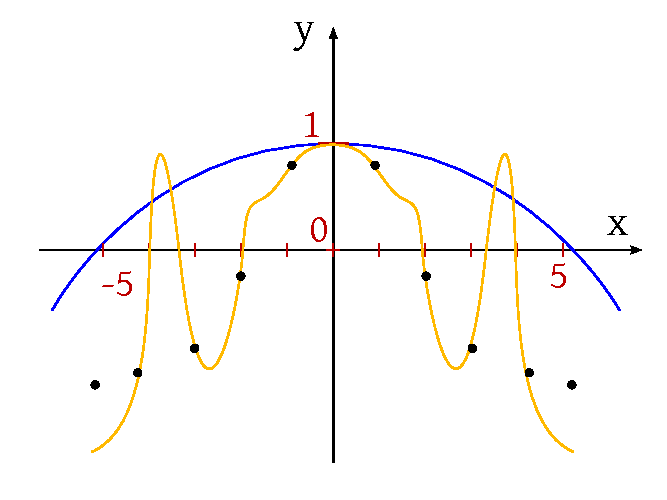
\includegraphics{img/01_runge_function.pdf}
      \caption{Runge's function (1901) illustrates the problem of oscillation at the edges of an interval that occurs when using polynomial interpolation with polynomials of high degree over a set of equispaced interpolation points}
      \label{img:runge}
    \end{center}
  \end{figure}

  Compare with Figure~\ref{img:runge}.

  Matrix $A_n$ is badly conditioned. Hence, small changes on the right side trigger a huge change in the solution.
\end{example}

Question: Is interpolation \emph{without} linear equation systems?


Approach:
\[ f_n(x) = \sum_{k=0}^n a_k x^k = \sum_{k=0}^n d_k \varphi_k(x) \]
with $\varphi_k(x) = x^k$.
\[ f_i = f_n(x_i) = \sum_{k=0}^k a_k \varphi_k(x_i) \]
\[
  \begin{pmatrix}
    \varphi_0(x_0) & \varphi_1(x_0) & \dots & \varphi_n(x_0) \\
    \varphi_0(x_1) & \varphi_1(x_1) & \dots & \varphi_n(x_1) \\
    \vdots & & & \vdots \\
    \varphi_0(x_n) & \varphi_1(x_n) & \dots & \varphi_n(x_n)
  \end{pmatrix}
  \begin{pmatrix}
    a_0 \\ a_1 \\ \vdots \\ a_n
  \end{pmatrix}
  =
  \begin{pmatrix}
    f_0 \\ f_1 \\ \vdots \\ f_n
  \end{pmatrix}
\]
\[ \varphi_k(x) \varphi_k(x_l) = \delta_{k,l} = \begin{cases} 1 & k=l \\ 0 & \text{else} \end{cases} \]

$\varphi_k$ polynomial of degree $n$
\[
  \varphi_k(x) = \frac{(x - x_0) (x - x_1) \dots (x - x_{k-1}) (x - x_{k+1}) \dots (x - x_n)}{(x_k - x_0) (x_k - x_1) \dots (x_k - x_{k-1}) (x - x_{k+1}) \dots (x_k - x_n)}
\] \[
  L_k^n(x) = \prod_{\substack{l = 0 \\ l \neq k}}^n \frac{x - x_l}{x_k - x_l} \qquad \text{\enquote{Lagrange polynomials}}
\]
Compare with Figure~\ref{img:lagrange-poly}

\begin{figure}[!h]
  \begin{center}
    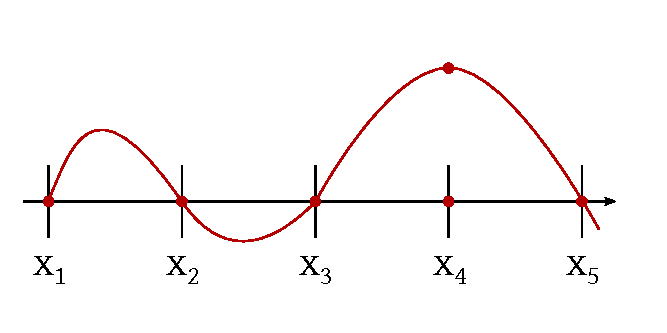
\includegraphics{img/02_lagrange_polynomial.pdf}
    \caption{Lagrange polynomials $L_3^4(x)$}
    \label{img:lagrange-poly}
  \end{center}
\end{figure}

Therefore, we get the interpolation polynomials
\[ f_n(x) = \sum_{k=0}^n f(x_k) \cdot L_k^n(x) \]

\begin{example}
  \begin{align*}
    f(x) &= \frac{1}{1 + x^2} \qquad x_0 = -5, x_1 = 0, x_2 = 5, n = 3 \\
    L_0^2(x) &= \frac{(x - x_1) (x - x_2)}{(x_0 - x_1) (x_0 - x_2)} = \frac{x (x - 5)}{-5 \cdot (-10)} = \frac{1}{50} x ( x - 5) \\
    L_2^2(x) &= \frac1{50} x (x + 5) \\
    L_1^2(x) &= \frac{(x - x_0) (x - x_2)}{(x_1 - x_0) (x_1 - x_2)} = -\frac1{25} (x^2 - 25) = \frac{1}{25} (25 - x^2) \\
    f_2(x) &= \frac1{26} \cdot \frac1{50} \cdot x \cdot (x - 5) + \frac1{25} (25 - x^2) + \frac1{26} \cdot \frac1{50} \cdot x \cdot (x + 5) \\
    &= 1 + x \cdot \left(-\frac{5}{26 \cdot 50} + \frac{5}{26 \cdot 50}\right) + x^2 \cdot \left(\frac{1}{26} \cdot \frac{1}{25} - \frac{1}{25}\right) \\
    &= 1 - \frac{1}{26} x^2
  \end{align*}
\end{example}

\begin{theorem}
  For $n \in \mathbb N$ let $(x_i)_0^n \in [a,b]$ be pairwise distinct supporting points.
  Let $f(x)$ be $n+1$ times differentiable. Then it holds that,
  \[ f(x) - f_n(x) = \frac{1}{(n+1)!} f^{(n+1)}(\xi(x)) \prod_{i=0}^n (x - x_i) \]
  with some proper intermediate value $\xi(x)$.
\end{theorem}

\begin{proof}
  Let $x=x_i$, the theorem is satisfied trivially.

  Let $\bar{x} \in [a,b], \bar{x} \neq x_i$ and $i = 0,\dots,n$ be arbitrary, but fixed.

  \begin{definition}
    \[ g_{\alpha}(x) = f(x) - f_n(x) - \alpha \prod_{i=0}^n (x - x_i), \alpha \in \mathbb R \]
    \[ g_\alpha(x_j) = 0 \]
    Choose $\alpha = \bar{\alpha}$: $g_{\bar{\alpha}}(\bar{x}) = 0$.
    \[ \overline{a} = \frac{f(\bar{x}) - f_n(\bar{x})}{\prod_{i=0}^n (\bar{x} - x_i)} \]
  \end{definition}
  $g_{\bar{\alpha}}$ has roots $x_0, \dots, \bar{x}_n, \bar{x}$ (which are $n+2$ values).
  
  $f(x)$ is continuously differentiable, $f(a) = f(b) = 0$.
  \[ \implies \exists \eta \in (a,b): f'(\eta) = 0 \]
  by Rolle's Theorem. Hence, $g_{\bar{\alpha}}'(x)$ has $n+1$ pairwise distinct zeros.
  $g_{\bar{\alpha}}''(x)$ has $n$ pairwise different zeros.
  $g_{\bar{\alpha}}^{(n+2)}(x)$ has one zero $\xi = \xi(x_0, \dots, x_n, \bar{x})$.
  \[
    0 = g_{\bar{\alpha}}^{(n+1)}(\xi)
    = f^{(n+1)}(\xi) - \underbrace{f_n^{(n+1)}(\xi)}_{=0}
    - \alpha\left(\underbrace{\prod_{i=0}^n (x - x_i)}_{=(n+1)!}\right)_{x=\xi}^{(n+1)}
  \] \[
    \implies \bar{\alpha} = \frac{1}{(n+1)!} f^{n+1}(\xi)
  \] \[
    \implies f(\bar{x}) - f_n(\bar{x})
    = \bar{\alpha} \prod_{i=0}^n (x - x_i) \forall \bar{x}
  \]
\end{proof}

\textbf{Interpolation:}
\[ f(x), f_n(x), f_n(x_i) = f_i, x_i \in [a,b] = [0,1] \qquad i = 0, \dots, n \quad i \neq j \implies x_i \neq x_j \]
\[ f(x) - f_n(x) = \frac{1}{(n+1)!} f^{(n+1)}(\xi(x)) \prod_{i=0}^n (x - x_i) \]

\begin{corollary}
  \[ \max_{x \in [a,b]} \card{f(x) - f_n(x)} = \frac{1}{(n+1)!} \max_{x \in [a,b]} \card{f^{(n+1)}(\xi(x)) \prod_{i=0}^n (x - x_i)} \]
  \[ \le \frac{1}{(n+1)!} \max_{x \in [a,b]} \card{f^{(n+1)}(x)} \cdot \max_{x \in [a,b]} \card{\prod_{i=0}^n (x - x_i)} \]
  $\max_{x \in [a,b]} \card{f^{(n+1)}(x)} < \infty$
  \emph{regularity} or \emph{differentiability} of the function to interpolate (given by the task assignment).

  $\max_{x \in [a,b]} \card{\prod_{i=0}^n (x - x_i)}$ is the property resulting from choice of supporting points.

  Hence, the polynomial degree $n$ and the choice of supporting points is influenceable.
\end{corollary}

\begin{example}
  \[ [a,b] = [0, \frac\pi2] \qquad f(x) = \sin(x) \qquad \card{f^n(x)} \leq 1 \]
  \[ \implies \max_{x \in [a,b]} \card{f(x) - f_n(x)} \leq \frac{1}{(n+1)!} \underbrace{\max_{x \in [0, \frac\pi2]} \card{f^{(n+1)}(x)}}_{\leq 1} = \card{\prod_{i=0}^n (x - x_i)} \leq \dots \]
  Let $n = 1, x_0 = 0, x_1 = \frac\pi2$.
  \[ f_n(x) = \frac2\pi x \]
  \[ \max_{x \in [0, \frac\pi2]} \card{f(x) - f_1(x)} \leq \frac12 \max_{x \in [0, \frac\pi2]} x \cdot (\frac\pi2 - x) = \left(\frac\pi4\right)^2 \approx 0.3084 \]
  \[ \max_{x \in [0,\frac\pi2]} \frac{\sin(x) - \frac2\pi x} = 0.2105 \]
\end{example}

\begin{example}
  \[ f(x) = \sqrt{x}, x \in [0,1] \]
  Let $n=1, x_0=0, x_1=1, f_1(x) = x$.
  \[ \max_{x \in [0,1]} \card{f(x) - f_1(x)} \leq \max_{x \in [0,1]} \underbrace{\card{f''(x)}}_{<\infty} \cdot \underbrace{\max_{x \in [0,1]} x (1 - x)}_{=\frac12} \]
  \[ f(x) = x^{\frac12} \qquad f'(x) = \frac12 x^{-\frac12} \qquad f''(x) = -\frac14 \frac{1}{x^{\frac32}} \]
\end{example}

For $x \in [a,b], 0 < a < b$, we want to answer the question for choice of supporting points. In the error estimate, the following term occurs:
\[
  \max_{x \in [a,b]} \underbrace{\card{\prod_{i=0}^n (x - x_i)}}_{x^{n+1} + a_a x^n + \dots + a_0 = a_0 (\frac1{a_0} x^{n+1} + \dots + 1)} \to \min_{x_0, \dots, x_n}
\] \[
  \max_{[a,b]} \card{p_{n+1}(x)} \to \min_{p_{n+1}, a_{n+1} = 1}
\]
This motivates the following exercise:
\[
  \min_{p_{n+1} \in \pi_1^{n+1}}
  \max_{x \in [a,b]}
  \card{p_{n+1}(x)}
  \text{ with }
  \prod_1^{n+1} = \setdef{q_{n+1} \in \pi^{n+1}}{q_{n+1}(0) = 1}
\]
This is a min-max problem. This gives the Chebyshev polynomials:
\begin{itemize}
  \item solution of a differential equation
  \item orthogonal polynomials
  \item recursive definition
\end{itemize}

\subsection{The Chebyshev polynomials}

Recursive definition:
\[ T_0(x) = 1, T_1(x) = x, T_{k+1}(x) = 2x \cdot T_k(x) - T_{k-1}(x) \qquad x \in \mathbb R \]
\[ T_2(x) = 2x \cdot x - 1 = 2x^2 - 1, T_3(x) = 2x (2x^2 - 1) - x = 4x^3 - 3x \]

\begin{lemma}
  Let $x \in [-1,+1], k \in \mathbb N$.

  Then it holds that $T_k(x) = \cos(k \cdot \arccos(x))$
\end{lemma}

\begin{proof}
  For $k = 0$ and $k = 1$, it is immediate.
  For $k \geq 2$, this will be part of the practicals.
\end{proof}

\subsubsection{Properties}

\begin{itemize}
  \item $\card{T_k(x)} \leq 1$ if $x \in [-1,1]$
  \item $T_k(1) = 1, T_k(-1) = (-1)^k$
  \item Zeros: $T_k(x) = \cos(k \cdot \arccos(x)) = 0$.
    \[ k \cdot \arccos(x) = \frac\pi2  + l \pi \]
    \[ \implies x_l^k = \cos{\frac{(1 + 2l) \pi}{2k}} \qquad l=0,\dots,k-1 \]
\end{itemize}

Compare with Figure~\ref{img:cpp}.

\begin{figure}[!h]
  \begin{center}
    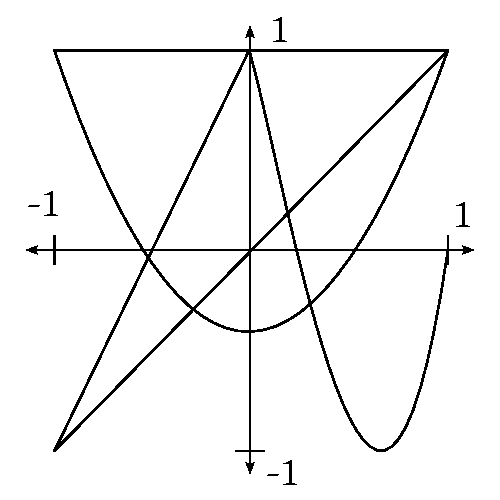
\includegraphics{img/03_chebyshev_polynomials_properties.pdf}
    \caption{Chebyshev polynomials properties}
    \label{img:cpp}
  \end{center}
\end{figure}

\begin{align*}
  T_k(x) &= +1 = k \cdot \arccos(x) = 2l\pi \\
  \implies \hat{x}_{2l}^k &= \cos\left(\frac{2l\pi}{k}\right) \\
  T_k(x) &= -1 \implies k \cdot \arccos(x) = (2l + 1) \pi \\
  \implies \hat{x}_{2l+1} &= \cos\left(\frac{(2l+1) \pi}{k}\right)
\end{align*}

\begin{remark}[An exercise for the practicals]
  Orthogonality of Chebyshev polynomials:
  \[
    \int_{-1}^1 \frac{T_l(x) T_k(x)}{\sqrt{1 - x^2}}
    = \begin{cases}
      0 & \text{if } k \neq l  \\
      \frac\pi2 & \text{if } k = l \neq 0 \\
      \pi & \text{if } k = l = 0
    \end{cases}
  \]
\end{remark}

\begin{lemma}
  \[
    T_k(x)
    = \frac12 \left[
      \left(x + \sqrt{x^2 - 1}\right)^k +
      \left(x - \sqrt{x^2 - 1}\right)^k
    \right]
    = \frac12 \left[
      (x + \sqrt{x^2 - 1})^k +
      (x + \sqrt{x^2 - 1})^{-k}
    \right]
  \]
\end{lemma}

\begin{proof}
  Let $k=0$. $T_0(x) = 1$. QED. \\
  Let $k=1$. $T_1(x) = x$.

  \begin{align*}
    T_{k+1}(x)
      &= 2x T_k(x) - T_{k-1}(x) \\
      &= 2x \frac12 \left[
        \left(x + \sqrt{x^2 - 1}\right)^k +
        \left(x - \sqrt{x^2 - 1}\right)^k
      \right] - \left[
        (x + \sqrt{x^2 - 1})^{k-1} +
        (x - \sqrt{x^2 - 1})^{k-1}
      \right] \\
      &= \frac12 \left(x + \sqrt{x^2 - 1}\right)^{k-1}
         \left[2x (x + \sqrt{x^2 - 1}) - 1\right]
       + \frac12 \left(x - \sqrt{x^2 - 1}\right)^{k-1}
         \left[2x (x - \sqrt{x^2 - 1} - 1\right] \\
      &= \frac12 \left(x + \sqrt{x^2 - 1}\right)^{k+1}
       + \frac12 \left(x - \sqrt{x^2 - 1}\right)^{k+1}
  \end{align*}
\end{proof}

\[
  \frac{(x - \sqrt{x^2 - 1})}{x + \sqrt{x^2 - 1}} \left(x + \sqrt{x^2 - 1}\right)
  = \frac{x^2 - (x^2 - 1)}{x + \sqrt{x^2 - 1}}
  = -\frac{1}{x + \sqrt{x^2 - 1}}
\]

Definition of Chebyshev polynomials:
$x \in [-1,1]$.
Interpolation task: $[a,b], 0 < a < b$.
This gives a min-max task for $p_n(x)$ with $p_n(0)=1$.
\[
  t \in [a,b]:
  x = \frac{b + a - 2t}{b - a} \qquad
  t = a: \quad x = 1 \qquad
  t = b: \quad x = -1
\]
Scaled Chebyshev polynomials:
\[
  \tilde{T_k}(t) = \frac{
    T_k\left(\frac{b + a - 2t}{b - a}\right)
  }{
    T_k\left(\frac{b + a}{b - a}\right)
  }
\]

\begin{theorem}
  Let $0 < a < b$.
  \[ \min_{\substack{p_n(t) \\ p_n(0)=1}} \max_{t \in [a,b]} \card{p_n(t)} \]
  \begin{align*}
    &= \max_{t \in [a,b]} \card{\tilde{T_n}(t)} = \frac{1}{T_n\left(\frac{b + a}{b - a}\right)} \\
    &= \frac{2q^n}{1 + q^{2n}} \text{ with } q = \frac{\sqrt b + \sqrt a}{\sqrt b - \sqrt a} > 1
  \end{align*}
\end{theorem}

\begin{proof}[Indirect proof]
  Assume there exists $q_n(t), q_n(0) = 1$ and
  \[ \max_{t \in [a,b]} \card{q_n(t)} < \max_{t \in [a,b]} \card{\tilde{T_n}(t)} \]

  \begin{align*}
    x &= \frac{b + a - 2t}{b - a} \iff t = \frac12 \left[ (b + a) - (b - a) x \right] \\
    x &= \cos{\frac{2l\pi}{n}} = \hat{x}_{2l}^n \implies T_n(x) = 1 \\
    \tilde{T_n}(t_{2l}^n) &= \frac{1}{T_n\left(\frac{b + a}{b - a}\right)} \\
    x &= \cos{\frac{(2l + 1) \pi}{n}} = \hat{x}_{2l+1}^n \implies T_n(\hat{x}_{2l+1}^n) = -1 \\
    \tilde{T_n}(\hat{t}_{2l+1}^n) &= -\frac{1}{T_n\left(\frac{b + a}{b - a}\right)} \\
    q_n\left(\hat{t}_{2l}^n\right) &< \frac{1}{T_n\left(\frac{b + a}{b - a}\right)} \\
    q_n(\tilde{t}_{2l}^n) &> -\frac{1}{T_n\left(\frac{b + a}{b - a}\right)}
  \end{align*}

  Compare with Figure~\ref{img:scpt}.

  \begin{figure}[b]
    \begin{center}
      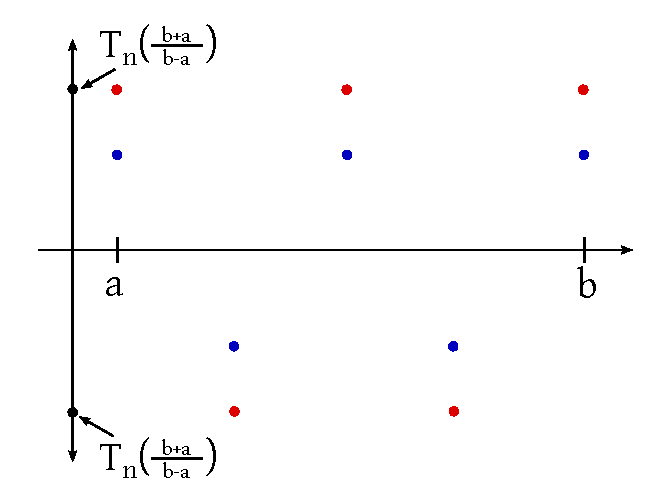
\includegraphics{img/03b_scaled_chebyshev_polynomials_theorem.pdf}
      \caption{Construction for proving the scaled Chebyshev polynomial theorem}
      \label{img:scpt}
    \end{center}
  \end{figure}

  \begin{align*}
    r_n(t) &= \tilde{T_n}(t) - q_n(t) \\
    \implies r(\hat{t}_{2l}^n) &> 0 \\
    t(\hat{t}_{2l+1}^n) &< 0
  \end{align*}

  $r_n(t)$ has $n$ zeros in $[a,b]$.
  \begin{align*}
    r_n(0) &= \tilde{T_n}(0) - q_n(0) = 0 \\
      &\implies n+1 \text{ zeros } \implies r_n(t) = 0 \forall t \\
      &\implies \tilde{T_n}(t) = q_n(t)
  \end{align*}
  This gives a contradiction.

  It remains to determine $T_n\left(\frac{b+a}{b-a}\right)$.
  \begin{align*}
    T_n\left(\frac{b+a}{b-a}\right)
      &= \frac12\left[q^n + q^{-n}\right] = \frac{q^{2n} + 1}{2q^n} \text{ with } q = \frac{b+a}{b-a} + \sqrt{\frac{(b+a)^2}{(b-a)^2} - 1} \\
      &= \frac1{b-a} \left[b + a + \sqrt{(b + a)^2 - (b - a)^2}\right] \\
      &= \frac1{b-a} \left[b + a + 2 \sqrt a \sqrt b\right] \\
      &= \frac{(\sqrt a + \sqrt b)^2}{(\sqrt b + \sqrt a)(\sqrt b - \sqrt a)} = \frac{\sqrt a + \sqrt b}{\sqrt b - \sqrt a}
  \end{align*}
\end{proof}

\begin{remark}
  This result also applies to the analysis of the so-called CG method (used to solve linear equation systems)
\end{remark}

Now consider the interpolation task in interval $[-1,1]$.
\[ f(x), f_n(x), f_n(x_i) = f(x_i) \qquad i = 0, \dots, n \]
Error estimate:
\[ \max_{x \in [-1,1]} \card{f(x) - f_n(x)} \leq \frac{1}{(n+1)!} \max_{x \in [-1,1]} \card{f^{(n+1)}(x)} \max_{x \in [-2,1] \card{\underbrace{\prod_{j=0}^n (x - x_j)}}_{p_{n+1}(x)}} \]

As supporting points, we choose the zeros $x_i$ of the $(n+1)$-th Chebyshev polynmial,
\[ T_{n+1}(x_i^{n+1}) = 0 \qquad T_{n+1}(x_i^{n+1}) = 0 \]
\[ T_{n+1}(x) = \prod_{j=0}^{n} (x - x_j^{(n+1)}) \cdot a_{n+1} = a_{n+1} x^{n+1} + \dots \]
We compute the first intermediate values:
\begin{align*}
  T_0(x) &= 1 \\
  T_1(x) &= x \\
  T_{k+1}(x) &= 2x T_k(x) - T_{k-1}(x) \\
  T_2(x) &= 2x^2 + \dots \\
  T_3(x) &= 4x^3 + \dots \\
  T_{k+1}(x) &= 2^k x^{k+1} + \dots
\end{align*}
We continue to consider $T_{n+1}(x)$:
\[ T_{n+1}(x) = 2^n x^{n+1} + \dots = \prod_{j=0}^n (x - x_j^{(n+1)}) = 2^{-n} T_{n+1}(x) \]
\[ \max_{x \in [-1,1]} \card{\prod_{j=0}^n (x - x_j^{(n+1)})} \leq 2^{-n} \]
By interpolation in the zeros of the Chebyshev polynomial, we get,
\[ \max_{x \in [-1, 1] \card{f(x) - f_n(x)}} \leq \frac{2^{-n}}{(n+1)!} \max_{x \in [-1,1]} \card{f^{(n+1)}(x)} \]
Extension to a general interval $[a,b]$ by transformation.

\begin{remark}
  This holds independent of the representation of the interpolation polynomial. For example with monom $x^k$. For example with Lagrange polynomials, but also with Chebyshev polynomials.
  \[ f_n(x) = \sum_{k=0}^n a_k T_k(x) \]
  \[ f_n(x_i^{(n+1)}) = \sum_{k=0}^n a_k T_k(x_i^{(n+1)}) = f(x_i^{(n+1)}) \]
\end{remark}

\begin{itemize}
  \item Fully occupied matrix (an exercise in the practicals):
    \[ \int_{-1}^1 \frac{T_k(x) T_l(x)}{\sqrt{1 - x^2}} \, dx = 0 \qquad k \neq l \]
  \item Discrete orthogonality
    \begin{itemize}
      \item direct computation of $a_k$
      \item Fast Fourier Transformation
    \end{itemize}
\end{itemize}

In the interpolation exercise, we have considered $n+1$ interpolation equations in pairwise different supporting points for determination of $n+1$ coefficients $a_k$ of $f_n$. We now have to determine an interpolation polynomial of degree $2n+1$ with $2(n+1)$ coefficients.
This gives $2(n+1)$ supporting points.

Our goal is $n+1$ supporting points.

Hence, we have 2 conditions per supporting point.

\[ f_{2n+1}(x_i) = f(x_i) \qquad f'_{2n+1}(x_i) = f'(x_i) \qquad i = 0, \dots, n \]

\subsection{Hermit interpolation}

Error estimation of a Hermit interpolation:

\[
  \max_{x \in [a,b]} \card{f(x) - f_{2n+1}(x)}
    \leq \frac{1}{(2n+2)!} \cdot \max_{x \in [a,b]} \card{f^{(2n+2)}(x)} \cdot \max_{x \in [a,b]} \card{\prod_{j=0}^n (x - x_j)^2}
\] \[
  f(x) - f_{2n+1}(x) = \underbrace{\frac{1}{(2n + 2)!} f^{2n+2}(\xi)}_{\alpha} \prod_{j=0}^n (x - x_j)
\] \[
  f(x) = f_{2n+1}(x) + \alpha \prod_{j=0}^n (x - x_j)^2
\]

$2n + 2$ zeros.
\[ x_0, \dots, x_n, \bar{x}, q(\bar{x}) = 0 \]

\textbf{Global interpolation tasks:}
\[ f(x), x \in [a,b], f_n(x), n \sim \text{ polynomial degree} \]
\[ f_n(x_i) = f(x_i) \qquad i = 1, \dots,n \]
\[ \max_{x \in [a,b]} \card{f_n(x) - f(x)} \leq \frac{1}{(n+1)!} \underbrace{\max_{x \in [a,b]} \card{f^{(n+1)}(x)}}_{\substack{\text{regularity of } f(x) = \sqrt{x} \\ x \in [0,1]}} \]
\[ \max_{x \in [a,b]} \card{\prod_{i=1}^n (x - x_i)} \]

\textbf{Question:} Local interpretation with polynomials of low degree.

\section{Piecewise linear interpolation} % 1.5

\[ [a,b], n \in \mathbb N, h = \frac{b - a}{n} \text{ step size} \]
Uniform supporting points $x_k = a + kh$. Compare with Figure~\ref{img:pli}.
\begin{figure}[!h]
  \begin{center}
    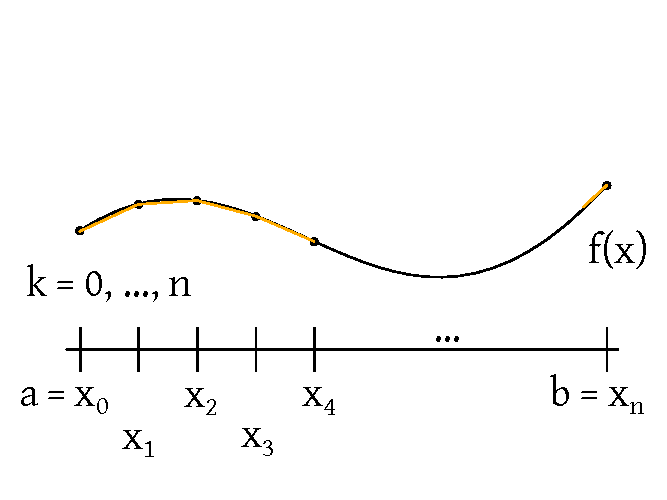
\includegraphics{img/03c_piecewise_linear_interpolation.pdf}
    \caption{Piecewise linear interpolation}
    \label{img:pli}
  \end{center}
\end{figure}

For \emph{every} interval $[x_{k-1}, x_k]$, $k=1,\dots,n$ we consider a local interpolation task. In the easiest case, this is a linear interpolation with
\[ f_n(x_{k-1}) = f(x_{k-1})  \qquad  f_n(x_k) = f(x_k) \]
This implies global continuity, but globally there is no continuous differentiability.

What is the error estimation?
\[
  \max_{x \in [x_{k-1},x_k]} \card{f(x) - f_n(x)}
  \leq \frac12 \max_{x \in [x_{k-1}, x_k]} \max\card{f''(x)}
  \cdot \underbrace{\max_{x \in [x_{k-1}, x_k]} \card{\underbrace{(x - x_{k-1})}_{\frac{h}2} \cdot \underbrace{(x - x_k)}_{\frac{h}2}}}_{\text{is given at } \frac12(x_{k-1} + x_k)}
  = \frac18 h^2 \max_{x \in [x_k, x_{k-1}]} \card{f''(x)}
\] \[
  \implies \max_{x \in [a,b]} \card{f(x) - f_n(x)} \leq \frac18 h^2 \max_{x \in [a,b]} \card{f''(x)}
\]
if $\card{f''(x)}$ is bounded, $f(x) = \sqrt{x}$.

How about the error estimation in other norms? E.g.
\[
  \int_a^b \left[f(x) - f_n(x)\right]^2 \, dx
  = \sum_{k=1}^n \int_{x_{k-1}}^{x_k} \left[f(x) - f_n(x)\right]^2 \, dx
\] \[
  x \in [x_{k-1}, x_k] \qquad f_n(x):
  f(x_{k-1}) = f_n(x_{k-1}) \qquad f(x_k) = f_n(x_k)
\] \[
  f_n(x) = f(x_{k - 1}) + \frac{f(x_k) - f(x_{k-1})}{h} (x - x_{k - 1})
\]
$x \in [x_{k-1}, x_k], x \in [x_{k-1}, \frac{x_{k-1} + x_k}{2}$
\[
  f(x) - f_n(x) = f(x) - f_n(x) - \underbrace{\left[f(x_{k-1}) - f_n(x_{k-1})\right]}_{=0}
  = \int_{x_{k-1}}^x \left[f'(s) - f_n'(s)\right] \, ds
\] \begin{align*}
  \left[f(x) - f_n(x)\right]^2
    &= \left[\int_{x_{k-1}}^x \mathbf 1 \cdot \left[f'(s) - f_n'(s)\right] \, ds\right]^2 \\
    &\underbrace{\leq}_{\text{Cauchy-Schwarz}} \int_{x_{k-1}}^x 1^2 \, ds \cdot \int_{x_{k-1}}^x \left[f'(s) - f_n'(s)\right]^2 \, ds \\
    &\leq (x - x_{k-1}) \cdot \int_{x_{k-1}}^{\frac{(x_{k-1} + x_k)}{2}} \left[f'(s) - f_n'(s)\right]^2 \, ds \\
  \implies \int_{x_{k-1}}^{\frac{x_{k-1} + x_k}{2}} \left[f(x) - f_n(x)\right]^2 \, dx
    &\leq \underbrace{\int_{x_{k-1}}^{\frac{x_{k-1} + x_k}{2}} (x - x_{k-1}) \, dx}_{\left.\frac12 (x - x_{k-1})^2 \right|_{x_{k-1}}^{\frac{x_k - x_{k-1}}{2}} = \frac{h^2}{8}} \cdot {\frac{x_{k-1} + x_k}{2}} \left[f'(x) - f_n'(x)\right]^2 \, dx
\end{align*}
Analogously, it follows that
\[ \int_{\frac{x_k + x_{k-1}}{2}}^{x_k} \left[f(x) - f_n(x)\right]^2 \, dx \leq \frac{h^2}{8} \int_{\frac{x_{k-1} + x_k}{2}}^{x_k} \left[f'(x) - f_n'(x)\right]^2 \, dx \]
\[ \implies \int_{x_{k - 1}}^{x_k} \left[f(x) - f_n(x)\right]^2 \leq \frac{h^2}{8} \int_{x_{k-1}}^{x_k} \left[f'(s) - f'_n(s)\right] \, ds \leq \frac{h^4}{24} \int_{x_{k-1}}^{x_k} \left[f''(s)\right]^2 \, ds \]
We will see later, that this inequality holds.

\[ f'_n(s) = \frac1h \left[f(x_k) - f(x_{k-1})\right] \]

Piecewise linear interpolation:
\[ [a,b], n \in \mathbb N, h = \frac{b - a}{n}, x_k = a + k \cdot h \]
$x \in [x_{k-1}, x_k]$
\[ f_n(x) = f(x_{k-1}) + \frac{x - x_{k-1}}{h} \cdot \left[f(x_k) - f(x_{k-1})\right] \]
\[
  \int_{x_{k-1}}^{x_k} \left[f(x) - f_n(x)\right]^2 \, dx
  \leq \frac18 h^2 \int_{x_{k-1}}^{x_k} \left[f'(x) - f_n'(x)\right]^2 \, dx
\]

Sidenote:
\[
  \frac1h \int_{x_{k-1}}^{x_k} \left[f'(s) - f_n'(s)\right] \, ds
  = \left.\frac1h \underbrace{\left[f(s) - f_n(s)\right]}_{=0}\right|_{x_{k-1}}^{x_k} = 0
\]

\begin{align*}
  \left[f'(x) - f_n'(x)\right]
    &= \int_{x_{k-1}}^{x_k} \left[f'(x) - f'_n(x) - \frac1h \int_{x_{k-1}}^{x_k} f'(s) - f'_n(s) \, ds\right]^2 \, dx \\
    &= \frac1h \int_{x_{k-1}}^{x_k} \left[f'(x) - f'_n(x)\right] \, ds \\
    &= \frac{1}{h^2} \int_{x_{k-1}}^{x_k} \left[\int_{x_{k-1}}^{x_k} \left[[f'(x) - f_n'(x)] - [f'(s) - f'_n(s)]\right] \, ds\right]
\end{align*}

\[ \int_a^b g'(s) \, ds = g(b) - g(a) \]

\begin{align*}
  \left[f'(x) - f_n'(x)\right]
    &= \frac1{h^2} \int_{x_{k-1}}^{x_k} \left[
      \int_{x_{k-1}}^{x_k} \int_s^x f''(\eta) - \underbrace{f''_n(\eta)}_{=0 \text{ because } f_n \text{ is linear}}
    \, d\eta \, ds \right]^2 \, dx \\
    &= \frac{1}{h^2} \cdot \int_{x_{k-1}}^{x_k} \left[\int_{x_{k-1}}^{x_k} \mathbf 1 \cdot \int_s^x f''(\eta) \, d\eta \, ds\right]^2 \, dx \\
\end{align*}

\[
  \int_a^b f \cdot g \, dx \le \left(\int_a^b f^2\right)^{\frac12} \cdot \left(\int_a^b g^2\right)^{\frac12}
\]

\begin{align*}
  \left[\int_{x_{k-1}}^{x_k} 1 \int_s^x f''(\eta) \, d\eta \, ds\right]^2
    &\leq \int_{x_{k-1}}^{x_k} 1^2 \, ds \int_{x_{k-1}}^{x_k} \left[f''(\eta) \, d\eta\right]^2 \, ds \\
    &\leq \frac1h \int_{x_{k-1}}^{x_k} \int_{x_{k-1}}^{x_k} \underbrace{\left[\int_0^x \mathbf 1 \cdot f''(\eta) \, d\eta \right]^2}_{\leq \card{\underbrace{\int_s^x 1^2 \, d\eta}_{= (x - s)}} \cdot \card{\int_s^x f''(\eta)^2 \, d\eta}} \, ds \, dx \\
    &\leq (x - s) \underbrace{\int_{x_{k-1}}^{x_k} [f(\eta)]^2 \, d\eta}_{\text{independent of } x, s} \\
    &\leq \frac1h \int_{x_{k-1}}^{x_k} \int_{x_{k-1}}^{x_k} \card{x - s} \, ds \, dx \cdot \int_{x_{k-1}}^{x_k} \left[f''(\eta)\right]^2 \, d\eta \\
  \intertext{$\hat{x} = x - x_{k-1}, \hat{s} = s - x_k - 1$} \\
  \int_{x_{k-1}}^{x_k} \int_{x_{k-1}}^{x_k} \card{x - s} \, ds \, dx
    &= 2 \cdot \int_{x_{k-1}}^{x_k} \int_{x_{k-1}}^{x} (x - s) \, ds \, dx \\
    &= 2 \cdot \int_0^h \underbrace{\int_0^x (x - s) \, ds}_{= \left. -\frac12 (x - s)^2 \right|_0^x = \frac12 x^2} \, dx \\
    &= \int_0^h x^2 \, dx = \frac13 h^3
\end{align*}

Result:
\begin{align*}
  \int_{x_{k-1}}^{x_k} \left[f'(x) - f'_n(x)\right]^2 \, dx
    &\leq \frac13 h^2 \cdot \int_{x_{k-1}}^{x_k} \left[f''(x)\right]^2 \, dx
\end{align*}

By insertion, we get
\[
  \int_{x_{k-1}}^{x_k} \left[f(x) - f_n(x)\right]^2 \, dx
  \leq \frac1{24} h^4 \cdot \int_{x_{k-1}}^{x_k} \left[f''(x)\right]^2 \, dx
\]
Local for all $k$
\[
  \int_a^b \left[f(x) - f_n(x)\right]^2 \, dx
  \leq \frac1{24} h^4 \int_a^b \left[f''(x)\right]^2 \, dx
\]

Norm for square-integrable functions:
\[
  \norm{f}_{L^2([a,b])} \coloneqq \left(\int_a^b [f(x)]^2 \, dx\right)^{\frac12} < \infty
\]

\[ \norm{f - f_n}_{L^2([a,b])} \leq \frac{1}{\sqrt{24}} h^2 \cdot \norm{f''}_{L^2([a,b])} \]
$\to 0$ for $k \to 0 \iff n \to \infty$.

\textbf{Requirement:} $\norm{f''}_{L^2([a,b])} < \infty$

Is not applicable for $f(x) = \sqrt{x}, x \in [0,1]$.
\[
  \norm{f' - f'_n}
  \leq \frac{1}{\sqrt{3}} h \norm{f''}_{L^2 \in ([a,b])}
\] \[
  x \in [x_{k-1}, x_k]:
  f_n(x) = f(x_{k-1}) + \frac{x - x_{k-1}}{h} \left[
    f(x_k) - f(x_{k+1})
  \right]
\] \[
  f'_n(x) = \frac1h \left[f(x_k) - f(x_{k-1})\right]
    = \frac1h \int_{x_{k-1}}^{x_k} f'(s) \, ds
\]

Recognize that $(a - b)^2 \leq 2(a^2 + b^2)$, then
\[
  \int_{x_{k-1}}^{x_k} \left[\underbrace{f'(x)}_{a} - \underbrace{f_n'(x)}_{b}\right]^2
    \leq 2 \cdot \int_{x_{k-1}}^{x_k} f'(x)^2 \, dx
      + 2 \cdot \int_{x_{k-1}}^{x_k} \underbrace{f'_n(x)^3}_{\left[\frac1h \int_{x_{k-1}}^{x_k} f'(s) \, ds\right]^2} \, dx
\]
with
\[
  \left[\frac1h \int_{x_{k-1}}^{x_k} f'(s) \, ds\right]^2
  \leq \frac1h 2 \underbrace{\int_{x_{k-1}}^{x_k} 1^2 \, ds}_{h}
  \int_{x_{k-1}}^{x_k} \left[f'(s)\right]^2 \, ds
\]
Hence,
\[
  \int_{x_{k-1}}^{x_k} \left[\underbrace{f'(x)}_{a} - \underbrace{f_n'(x)}_{b}\right]^2
  \leq 4 \cdot \int_{x_{k-1}}^{x_k} \left[f'(x)\right]^2 \, dx
\]

\begin{align*}
  \norm{f' - f'_n}_{L^2([a,b])} &\leq 2 \cdot \norm{f'}_{L^2([a,b])} \\
  \norm{f - f_n}_{L^2([a,b])} &\leq \frac1{\sqrt2} \cdot h \norm{f'}_{L^2([a,b])}
\end{align*}

In general, it holds that
\[ \tau = 0,1 \qquad s = 1,2 \qquad s = p+1 \qquad p = \operatorname{grad}(f_n) \]
\[ \norm{f^{(\tau)} - f_n^{(\tau)}}_{L^2([a,b])} \leq c(s, \tau) h^{s-\tau}\norm{f^{(s)}}_{L^2([a,b])} \]

\begin{align*}
  \int_{x_{k-1}}^{x_k} \left[f'(x) - f'_n(x)\right]^2 \, dx
    &= \int_{x_{k-1}}^{x_k} \left[f'(x) - \frac1h \int_{x_{k-1}}^{x_k} f'(s) \, ds\right]^2 \, dx \\
    &\leq h^{2\sigma} \cdot \int_{x_{k-1}}^{x_k} \int_{x_{k-1}}^{x_k} \frac{f'(x) - f'(s)}{\card{x + s}^{1 + 2\sigma}} \, ds \, dx \\
    &= \frac1{h^2} \int_{x_{k-1}}^{x_k} \left[ \int_{x_{k-1}}^{x_k} \left[f'(x) - f'(s) \right] \, ds \right]^2 \, dx \\
    &= \frac1{h^2} \left[\int_{x_{k-1}}^{x_k} \frac{f'(x) - f'(s)}{\card{x - s}^{\frac12 + \sigma}} \card{x - s}^{\frac12 + \sigma} \, ds\right]^2 \\
    &\leq \int_{x_{k-1}}^{x_k} \frac{{f'(x) - f'(s)}^2}{\card{x - s}^{1 + 2\sigma}} \, ds \cdot \underbrace{\int_{x_{k-1}}^{x_k} \card{x - s}^{1 + 2\sigma} \, ds}_{\leq h \cdot h^{1 + 2\sigma}} \\
  \norm{f' - f'_n}_{L^2([a,b])}
    &\leq h^\sigma \norm{f}_S \\
  \norm{f}_s^2 &\coloneqq \int_a^b \int_a^h \frac{(f'(x) - f'(s))^2}{\card{x - s}^{1 + 2\sigma}} \, ds \, dx  & s \in (1,2), \sigma = s - 1 \\
    &= h^{s - 1} \norm{f}_s
\end{align*}

\begin{theorem}
  Let $f(x), x \in [a,b]$ be given with $\card{f}_s < \infty$, where,
  \[
    \card{f}_1^2 = \int_a^b [f'(x)]^2 \, dx \qquad
    \card{f}_2^2 = \int_a^b [f''(x)]^2 \, dx \qquad 1 < s < 2
  \] \[
    \card{f}_s = \int_a^b \int_a^b \frac{f'(x) - f'(s)}{\card{x - s}^{1 + 2\sigma}} \, ds \, dx
  \]
  Let $f_n(x)$ be the piecewise linear interpolation polynomial with
  \[ f(x_k) = f_n(x_k) \qquad x_k = a + k \cdot h \qquad h = \frac{b - a}{n} \]
  Then it holds that
  \[
    \norm{f - f_n}_{\tau} \leq c(s, \tau) \cdot h^{s - \tau} \cdot \card{f}_s
  \]
  with
  \[
    \norm{f}_0^2 = \int_a^b [f(x)]^2 \, dx \qquad
    \norm{f}_1^2 = \int_a^b [f'(x)]^2 \, dx
  \]
\end{theorem}

Proof for $\tau \in \set{0,1}, s \in \set{1,2}$.

\begin{remark}
  \begin{itemize}
    \item $\tau \in (0,1)$
      \[ \norm{f}_\tau^2 = \int_a^b \int_a^b \underbrace{\left[f(x) - f(s)\right]^2}_{\card{x - s}^{1 + 2\sigma}} \, ds \, dx \]
    \item The estimation stays correct for $0 \leq \tau < \frac32$.
      \[ \tau \leq s \leq \underbrace{p + 1}_{\text{polynomial degree}} \]
      \[ s > \frac12 \]
      This assumes that $f(x)$ is continuous.
  \end{itemize}
\end{remark}

Error estimation:
\[ \int_a^b \left[f(x) - f_n(x)\right]^2 \, dx \leq \frac1{24} \underbrace{\sum_{k=1}^n (x_k - x_{k-1})^4}_{[T_1]} \cdot \int_{x_{k-1}}^{x_k} \underbrace{[f''(x)]^2}_{[T_2]} \, dx \]
Here terms $T_1$ and $T_2$ balance out each other. If $T_1$ is large, $T_2$ will be \enquote{small}.  If $T_1$ is small, $T_2$ will be \enquote{large}.

\[ f(x) = \sqrt{x}, x \in [0,1], s < 1 \]

\dateref{18th of October 2017}

\section{Piecewise linear interpolation}

\[ f(x), x \in [a,b], a = x_0 < x_1 < \ldots < x_n = b \]
\[ f_n(x); x \in [x_{k-1}, x_k] \]

\begin{align*}
  f_n(x) &= f(x_{k-1}) + \frac{x - x_{k-1}}{x_k - x_{k-1}} \left[f(x_k) - f(x_{k-1})\right] \\
         &= \left[ 1 - \frac{x - x_{k-1}}{x_k - x_{k-1}} \right] f(x_{k-1}) + \frac{x - x_{k-1}}{x_k - x_{k-1}} f(x_k) \\
         &= \frac{x_k - x}{x_k - x_{k-1}} f(x_{k-1}) + \frac{x - x_{k-1}}{x_k - x_{k-1}} f(x_k)
\end{align*}

For $x \in [x_k, x_{k+1}]$
\[ f_n(x) = \frac{x_{k+1} - x}{x_{k+1} - x_k} f(x_k) + \frac{x - x_k}{x_{k+1} - x_k} f(x_{k+1}) \]

So we can find a representation, such that:

\[ f_n(x) = \sum_{k=0}^n f(x_k) \varphi_k(x) \qquad x \in [a,b] \]

with the basis functios
\[
  \varphi_k(x) = \begin{cases}
    \frac{x - x_{k-1}}{x_k - x_{k-1}} & x \in [x_{k-1}, x_k] \\
    \frac{x_{k+1} - x}{x_{k+1} - x_k} & x \in [x_k, x_{k+1}] \\
    0 & \text{else}
  \end{cases}
\]

% \pic{img/basis\_function.pdf}{Visualization of the interpolation's basis functions}

\begin{figure}[t]
  \begin{center}
    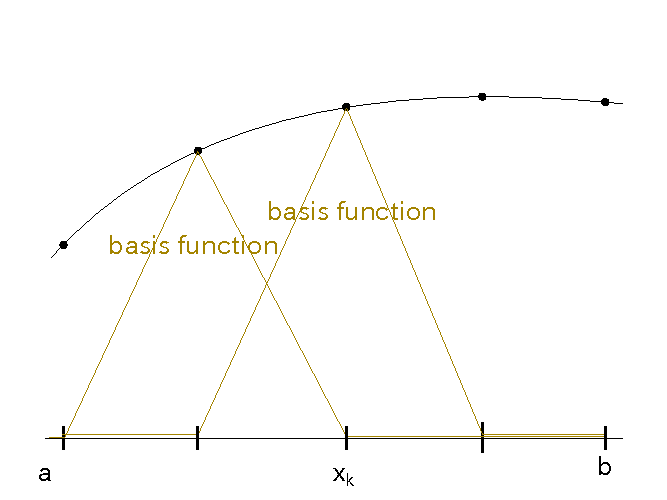
\includegraphics{img/basis_function.pdf}
    \caption{Visualization of the interpolation's basis functions}
  \end{center}
\end{figure}

Our basis functions satisfy:

\[
    \varphi_k(x) = \begin{cases}
        1 & x = x_k \\
        0 & x = x_l \neq x_k
    \end{cases}
\]

\enquote{Lagrange bases} satisfy such a property. Hence our basis functions are also called \emph{Lagrange bases}.
\begin{figure}[t]
  \begin{center}
    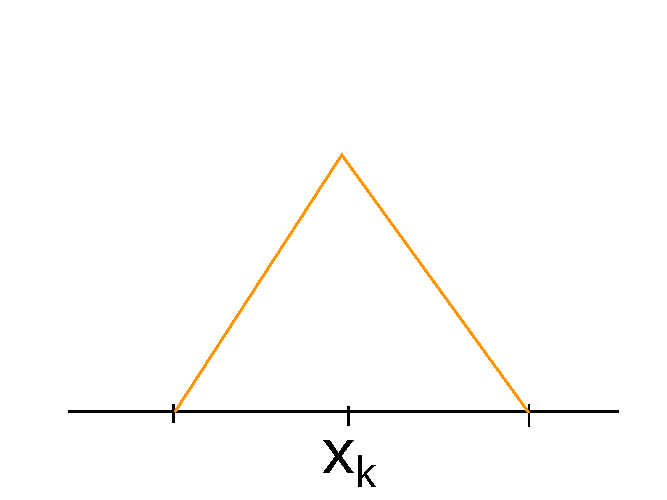
\includegraphics{img/lagrange_basis.pdf}
    \caption{Visualization of Lagrange bases}
  \end{center}
\end{figure}

The functions
\[ \frac{x - x_{k-1}}{x_k - x_{k-1}}, \frac{x_{k+1} - x}{x_{k+1} - x_k} \]
are called \enquote{form functions}.

We can generalize this to two dimensions. We get a so-called \enquote{hat function}.

\begin{figure}[t]
  \begin{center}
    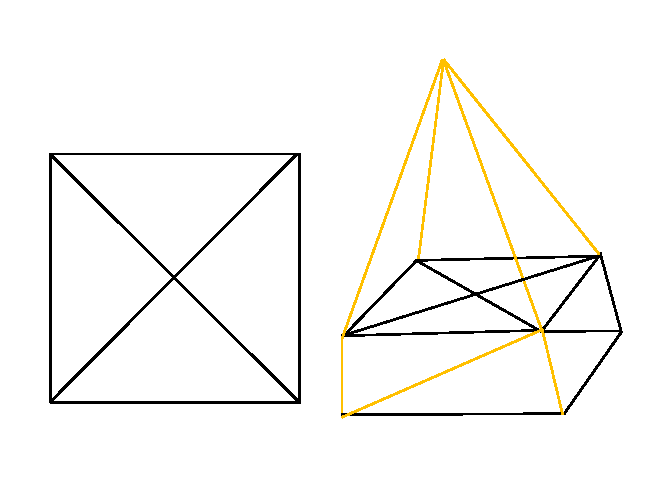
\includegraphics{img/hat_function.pdf}
    \caption{Visualization of a hat function}
  \end{center}
\end{figure}

Interpolating function
\[ f_n(x) = I_n \]
\[ f(x) \coloneqq \sum_{k=0}^n f(x_k) \varphi(x) \]

Error estimation
\[ \| f - I_n f \|^2_{L^2([a,b])} \leq \frac{1}{24} h^4 \| f'' \|^2_{L^2([a,b])} \]

Assuming this error estimation is optimal, is there another, piecewise linear function with smaller error?

In general, a representation of a piecewise linear function
\[ f_n(x) = \sum_{k=0}^n a_k \varphi_k(x) \]
and we consider the minimization problem
\[ \int_a^b \left[ f(x) - \sum_{k=0}^n a_k \varphi(x) \right]^2 \, dx \implies \text{min}_{a_0, \ldots, a_n} \]


\section{Projection methods} % 1.6

Minimization problem for the functional $F(\underline{a})$:
\begin{align*}
  F(\underline{a}) &\coloneqq \int_a^b \left[ f(x) - \sum_{k=0}^n a_k \varphi(x) \right]^2 \, dx \\
        &= \int_a^b \left[f(x) - \sum_{k=0}^n a_k \varphi(x) \right] \left[ f(x) - \sum_{l=0}^n a_l \varphi_l(x) \right]\, dx \\
        &= \int_a^b \left[f(x)\right]^2 \, dx - 2 \cdot \sum_{k=0}^n a_k \underbrace{\int_a^b f(x) \varphi_k(x) \, dx}_{f_k \coloneqq}
           + \sum_{k=0}^n \sum_{l=0}^n a_k a_l \underbrace{\int_a^b \varphi_k(x) \varphi_l(x) \, dx}_{m_{kl} = m_{lk} \coloneqq}
\end{align*}

\[ F(\underline{a}) = \int_a^b \left[f(x)\right]^2 \, dx - 2 \sum_{k=0}^n f_k a_k + \sum_{k=0}^n \sum_{l=0}^n m_{kl} a_k a_l \]
is a quadratic function at coefficient $q_k$.

A necessary condition for the minimum is:
\[ \frac{\partial}{\partial a_j} F(\underline{a}) = 0, j = 0,n \]

\[ 0 \stackrel{!}{=} \frac{\partial}{\partial a_j} F(\underline{a}) = \frac{\partial}{\partial a_j} \left[ \int_a^b \left[f(x)\right]^2 \, dx - 2 \sum_{k=0}^n f_k q_k + \sum_{k=0}^n \sum_{l=0}^n m_{kl} a_k a_l \right] \]
as $\frac{\partial}{\partial a_j}(\int_a^b \left[f(x)\right]^2) = 0$ and $\sum_{k=0}^n f_k q_k = f_0 a_0 + f_1 a_1 + \ldots + f_j a_j + \ldots$, we get
\begin{align*}
  &= -2 f_j + \frac{\partial}{\partial a_j} \left[ \sum_{l=0}^n m_{jl} a_j a_l + \sum_{k\neq j} \sum_{l=0}^n m_{kl} a_k a_l \right] \\
  &= -2 f_j + \frac{\partial}{\partial a_j} \left[ m_{jj} a_j^2 + \sum_{l\neq j} m_{jl} a_j a_l + \sum_{k\neq j} m_{kj} a_k a_j + \sum_{k\neq j} \sum_{l \neq j} m_{kl} a_k a_l \right] \\
  &= -2 f_j + 2 m_{jj} a_j + \sum_{l\neq j} m_{jl} a_l + \sum_{k \neq j} m_{kj} a_k \\
  &= -2 f_j + 2 m_{jj} a_j + 2 \cdot \sum_{l\neq j} m_{jl} a_l \\
  &= 2 \left[ \sum_{l=0}^n m_{jl} a_l - f_j \right] \stackrel{!}{=} 0 \qquad j = 0,n
\end{align*}

Linear equation system:
\[ M \underline{a} = \underline{f} \]
\[ M[j,l] = \int_a^b \varphi_l(x) \varphi_j(x) \, dx \qquad \text{\enquote{mass matrix}, also called \enquote{Gram's matrix}} \]
\[ f_j = \int_a^b f(x) \varphi(x) \, dx \qquad \text{\enquote{load vector}} \] % translation of "Lastvektor"
Ritz' method.

\[ \sum_{l=0} m_{jl} a_l = f_j \]
\[ \sum_{l=0}^n a_l \int_a^b \varphi_l(x) \varphi_j(x) \, dx = \int_a^b f(x) \varphi(x) \, dx \]
\[ f_n(x) = \sum_{l=0}^n a_l \varphi_l(x) \]
\[ \int_a^b f_n(x) \varphi_j(x) \, dx = \int_a^b f(x) \varphi_j(x) \, dx \qquad \forall \varphi_j, j = 0, n \]
\[ j_n(x) = \sum_{j=0}^n b_j \varphi_j \]

\[ \int_a^b f_n(x) g_n(x) \, dx = \int_a^b f(x) g_n(x) \, dx \]

Ansatz space (or also trial space):
\[ V_n \coloneqq \operatorname{span}\left\{ \varphi_k(x) \right\}_{k=0}^n \]
Find $f_n \in V_n: \int_a^b f_n(x) g_n(x) \, dx = \int_a^b f(x) g_n(x) \, dx \quad \forall g_n \in V_n$.

This is a so-called \enquote{variation form} (dt. Variationsformulierung). Especially, it is a \enquote{Galerkin-Bubnov variation form} because Ansatz and test space are the same. % translation of Ansatzraum acc. to Steinbach

The solution $f_n(x) = Q_n f(x)$, projection, $L_2$ projection

\dateref{2017/10/23}

\[ I_n f(x) = \sum_{k=0}^n f(x_k) \varphi_k(x) \]

\begin{align*}
  \|f - f_n\|_{L^2([a,b])} &\leq \frac{1}{\sqrt{24}} h^2 \|f''\|_{L^2([a,b])} \\
  \|f' - f'_n\|_{L^2([a,b])} &\leq \frac{1}{\sqrt3} h \| f'' \|_{L^2([a,b])}
\end{align*}

\[ Q_nf: \| f - Q_n f \|^2_{L^2([a,b])} \to \min_{a_0,\ldots,a_n} \]

Linear equation system:
\[ \sum_{k=0}^n a_k \int_a^b \varphi_k(x) \varphi_l(x) \, dx = \int_a^b f(x) \varphi_l(x) \, dx \qquad l = 0, n \]

Does it have a unique solution?

Ansatz space $V_n = \operatorname{span}\{\varphi_k\}_{k=0}^n = S_k^1([a,b])$

Now we consider an arbitrary function $g_h \in V_h$.
\[ g_h \in V_h \Leftrightarrow g_h(x) = \sum_{k=0}^n g_k \varphi_k(x) \Leftrightarrow \underline{g} = (g_k)_{k=0}^n \in \mathbb R^{n+1} \]
Isomorphism: $g_h \in V_h \leftrightarrow g \in \mathbb R^{n+1}$.

\[ M_h \underline{a} = \underline{f} \]

What do we know about the matrix (to determine uniqueness of the solution)?

\[ M_h[l,k] = \int_a^b \varphi_k(x) \varphi_l(x) \, dx = M_h [k,l] \implies M_h = M_h^T \text{ symmetrical} \]

We test for positive definiteness:  % TODO: check 'definiteness'. correct word?
\begin{align*}
  g \in \mathbb R^{n+1}: \left(M_h \underline{g}, \underline{g}\right)
    &= \sum_{k=0}^n \sum_{l=0}^n M_h[l,k] g_k g_l \\
    &= \sum_{k=0}^n \sum_{l=0}^n g_k g_l \int_a^b \varphi_k(x) \varphi_l(x) \, dx \\
    &= \int_a^b \underbrace{\sum_{k=0}^n g_k \varphi_k(x)}_{g_h(x)} \underbrace{\sum_{l=0}^n g_l \varphi_l(x) \, dx}_{g_h(x)} \\
    &= \int_a^b \left[g_k(x)\right]^2 \, dx \geq 0 \\
  = 0 &\Leftrightarrow 0 = g_h(x) = \sum_{k=0}^n g_k \varphi_k(x) \Leftrightarrow g_0 = \ldots = g_n = 0, \underline{g} = \underline{0}
\end{align*}

\[ (M_h g, g) > 0 \quad \forall \underline{g}, \sum_{k=0}^n g_k^2 > 0 \]
$M_h$ is positive definite $\implies$ $M_h$ is invertible.

What is the layout of $M_h$ for piecewise linear basis functions.

\[
    \varphi_k(x) = \begin{cases}
      \frac{x - x_{k-1}}{x_k - x_{k-1}} & x \in (x_{k-1}, x_k) \\
      \frac{x_{k+1} - x}{x_{k+1} - x_k} & x \in (x_k, x_{k+1}) \\
      0 & \text{ otherwise}
    \end{cases}
\]
\[ M_k[l,k] = \int_a^b \varphi_k(x) \varphi_l(x) \, dx = 0 \text{ for } l+k, k \pm 1 \]

\begin{figure}[h]
  \begin{center}
    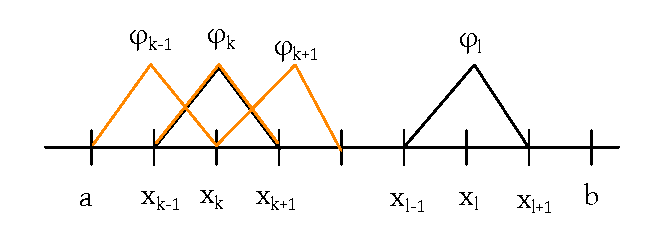
\includegraphics{img/04_layout_of_linear_basisfunctions.pdf}
    \caption{Layout of linear basis functions}
  \end{center}
\end{figure}

\[ l = k + 0, n \]
\begin{align*}
  M_h[K,k] &= \int_a^b[\varphi_k(x)]^2 \, dx = \int_{x_{k-1}}^{x_k} \left(\frac{x - x_{k-1}}{x_k - x_{k+1}}\right)^2 \, dx + \int_{x_k}^{x_{k+1}} \left(\frac{x_{k+1} - x}{x_{k+x} - x_k}\right)^2 \, dx \\
    &= \frac13 (x_k - x_{k-1}) + \frac13 (x_{k+1} - x_k) = \frac23 h \\
  M_h[0,0] &= \frac13(x_1 - x_0) = \frac13h \\
  M_h[n,n] &= \frac13(x_n - x_{n-1}) = \frac13 h
\end{align*}

\[ l = k \mp 1 \]
\begin{align*}
  M_h[k+1,k] &= \int_a^b \varphi_k(x) \varphi_{k+1}(x) \, dx \\
    &= \int_{x_k}^{x_{k+1}} \frac{x_{k+1} - x}{x_{k+1} - x_k} \frac{x - x_k}{x_{k+1} - x_k} \, dx \\
    &\underbrace{\underbrace{=}_{h_k = x_{k+1} - x_k}}^{s = x - x_k} \frac{1}{h^2} \int_0^{h_k} (h_k - s) s \, ds = \frac{1}{h_k^2} \left[\frac12 h_k s^2 - \frac13 s^2\right]^{h_k}_0
    &= (\frac12 - \frac13) h_k = \frac16 h_k
\end{align*}

\[ h = \frac{b-a}{h}, x_k = a + kh, k = 0,n \]

\[
   M_h =
   \frac16h \begin{pmatrix}
    2 & 1    & \ldots &        & 0 \\
    1 & 4    &        &        & \\
    \vdots & & \ddots &        & \vdots \\
      &      &        &        & 4 & 1 \\
    0 &      &        & \ldots & 1 & 2
  \end{pmatrix}
  \in \mathbb R^{(n+1) \times (n+1)}
\]

Properties of this matrix?
\begin{itemize}
  \item tridiagonal ($n=1$)
  \item diagonal dominant ($n=1$)
  \item $M_h = M_h^T > 0$ (hence symmetrical, positive definite)
  \item matrix has few non-zero values (weakly assigned):  % TODO: verify 'weakly assigned' wording
     \[ 2 + 3 (n - 1) + 2 = 3n + 1 \text{ non-zero values} \]
  \item The inverse matrix is not weakly assigned (has many non-zero values)
\end{itemize}

\[
  g_h \in V_k: (M_h g, g)
    = \int_a^b [g_h(x)]^2 \, dx
    = \sum_{k=1}^n \underbrace{\int_{x_{k-1}}^{x_k} \left[g_h(x)\right]^2 \, dx}_{\int_{x_{k-1}}^{x_k}} \left[g_{k-1} \frac{x_k - x}{x_k - x_{k-1}} + g_k\frac{x - x_{k-1}}{x_k - x_{k-1}}\right]^2 \, dx \]
\[ = g^2_{k-1} \int_{x_{k-1}}^{x_k} \left(\frac{x_k - x}{x_k - x_{k-1}}\right)^2 \, dx + 2 g_{k-1} g_k \underbrace{\int_{x_{k-1}}^{x_k} \frac{x_k - x}{x_k - x_{k-1}} \frac{x - x_{k-1}}{x_k - x_{k-1}}}_{\frac16 h_k} \, dx + g^2_k \underbrace{\int_{x_{k-1}}^{x_k} \left(\frac{x - x_{k-1}}{x_k - x_{k-1}}\right)^2}_{\frac13 h_k} \, dx \]
\[ = \frac16 h_k \left[2 g_{k-1}^2 + 2 g_{k-1} g_k + 2 g_k^2 \right] = \frac16 h_k \vec{\begin{pmatrix} 2 & 1 \\ 1 & 2 \end{pmatrix}\begin{pmatrix} g_{k-1} \\ g_k \end{pmatrix}}{\begin{pmatrix} g_{k-1} \\ g_k \end{pmatrix}} \]
where $\frac16 h_k \left(\begin{pmatrix} 2 & 1 \\ 1 & 2 \end{pmatrix}\right)$ is $M_{h,k}$ is the \emph{local} mass matrix. % TODO: masse matrix
$\frac{x_k - x}{x_k - x_{k-1}}$ and $\frac{x - x_{k-1}}{x_k - x_{k-1}}$ are the form functions.
\[ \implies M_h = \sum_{k=1}^n A_k^T M_{h,k} A_k \]

$n=2$
\[ M_{h,k} = \int_{\tau_k} \varphi_{k,l}(x) \varphi_{k,j}(x) \, dx \qquad i,j = 1,3 \]
\[ M_{h,k} = \frac{\operatorname{area}_k}{10} \begin{pmatrix} 2 & 1 & 1 \\ 1 & 2 & 1 \\ 1 & 1 & 2 \end{pmatrix} \]

$n=3$
\[ M_{h,k} = \begin{pmatrix} 2 & 1 & 1 & 1 \\ 1 & 2 & 1 & 1 \\ 1 & 1 & 2 & 1 \\ 1 & 1 & 1 & 2 \end{pmatrix} \]

\begin{figure}[h]
  \begin{center}
    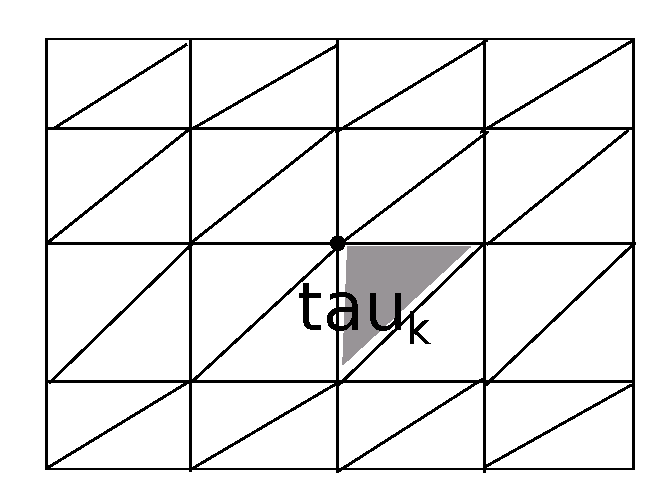
\includegraphics{img/05_area.pdf}
    \caption{Area}
  \end{center}
\end{figure}

Linear equation system:
\[ M_h \underline{a} = \underline{f} \quad \implies \text{ solution } \quad \underline{a} = M_h^{-1} \underline{f} \]
\[ \implies (Q_h f)(x) = \sum_{k=0}^n a_k \varphi_k(x) \]
$Q_n f$ is the solution of
\[ \int_a^b \left(Q_n f\right)(x) g_h(x) \, dx = \int_a^b f(x) g_h(x) \, dx \qquad \forall g_h \in \operatorname{span}\{\varphi_l\}^n_{l=0} \]
\[ \implies \int_a^b \left[f(x) - \left(Q_h f)(x)\right)\right] g_h(x) \, dx = 0 \forall g_h \in V_h \qquad \text{Galerkin orthogonality} \]
\begin{align*}
  \| f - Q_h f \|^2_{L^2([a,b])}
    &= \int_a^b \left[ f(x) - (Q_h f)(x) \right] \left[ f(x) - (Q f)(x) \right] \, dx \\
    &= \int_a^b \left[ f(x) - (Q_h f)(x) \right] f(x) \, dx - \underbrace{\int_a^b \left[f(x) - (Q_h f)(x)\right] Q_h f(x) (\text{something missing here?}) \, dx}_{=0, \text{ Galerkin orthogonality}} \\ % TODO
    &= \int_a^b \left[f(x) - (Q_h f)(x)\right] f(x) \, dx - \underbrace{\int_a^b \left[f(x) - (Q_h f)(x)\right] g_h(x) \, dx}_{=0} \\
    &= \int_a^b \left[f(x) - (Q_h f)(x)\right] \left[f(x) - g_h(x)\right] \, dx \\
    &\leq \| f - Q_h f \|_{L^2([a,b])} \| f - g_h \|_{L^2([a,b])} \\
  \implies \| f - Q_h f \|_{L^2([a,b])} &\leq \|f - g_h\|_{L^2([a,b])} \qquad \forall g_h \in V_h \\
  \| f - Q_h f \|_{L^2([a,b])} &\leq \inf_{g_h \in V_k} \| f - g_h \|_{L^2([a,b])}
\end{align*}

The last line corresponds to a minimization problem.
It's the so-called \emph{Cea's Lemma}.

\begin{lemma}[Cea's lemma]
  \[ \| f - Q_h f \|_{L^2([a,b])} \leq \inf_{g_h \in V_k} \| f - g_h \|_{L^2([a,b])} \]
\end{lemma}

\[
  \implies \|f - Q_h f \|_{L^2([a,b])} \leq \inf_{g_h} \| f - g_h \|_{L^2([a,b])} \\
    \stackrel{\leq}{g_h = I_h f} \|f - I_h f \|_{L^2([a,b])}
    \leq \frac{1}{\sqrt{24}} h^2 \| f'' \|_{L^2([a,b])}
\]

Given:
\[ \| f - Q_h f \|_{L^2([a,b])} \leq \| f - I_h f \|_{L^2([a,b])} \]
Find whether it holds that:
\[ \| f - I_h f \|_{L^2([a,b])} \leq c \|f - Q_h f \|_{L^2([a,b])} \]
This question is easy to answer for $n=1$, but an open research question for $n\geq 2$.

We can show that $c$ converges towards 1.
So we can show how interpolation and projection errors behave towards each other.

\[ \|f - Q_h f \|^2_{L^2([a,b])} = \int_a^b [f(x) - (Q_h f)(x)] f(x) \, dx \]
\[ \stackrel{\text{c.s.u.}}{\leq} \| f - Q_h f \|_{L^2([a,b])} \|f\|_{L^2([a,b])} \]
\[ \|f - Q_h f\|_{L^2([a,b])} \leq \|f\|_{L^2([a,b])} \]
$L_2$ projection is also well-defined for $f \in L^2([a,b])$,
hence also for non-continuous $f$. % TODO: 'non-continuous' =?= 'unstetig'

Error estimation:
\[ \| f - Q_h f \|_{L^2([a,b])} \leq \| f \|_{L^2([a,b])} \]
where $s = 0$.
\[ \| f - Q_h f \|_{L^2([a,b])} \leq \frac{1}{\sqrt{24}} h^2 \|f''\|_{L^2([a,b])} = c(s) h^2 \|f\|_s \qquad ,s = 2 \]
In terms of interpolation error: $s \in [1,2]$

\begin{theorem}
  $Q_h f$ is piecewise linear.
  \[ \| f - Q_h f \|_{L^2([a,b])} \leq c(s) h^s \|f\|_s, \qquad s \in [0,2] \]
  Interpolation $s > \frac12$.
\end{theorem}

Two major questions are left. We considered:
\[ \| f - I_h f \|_{L^2}, \quad \| f' - (I_h f)' \|_{L^2} \]
\[ \| f - Q_h f \|_{L^2} \leq \| f - I_h f \|_{L^2} \leq \ldots \]
First question:
\[ \| f' - (Q_h f)' \|_{L^2} \leq ? \]
Second question:
If we consider the $L^2$ projection,
\[ \int_a^b Q_h f g_h \, dx = \int_a^b f g_h \, dx \]
\[ g_h = Q_h f \]
\[ \implies \| Q_h f \|_{L^2([a,b])} \leq \| f \|_{L^2([a,b])} \]
This is called \emph{$L^2$ stability of the $L^2$ projection}.
This property does not hold for interpolation.
Interpolation is not $L^2$ stable.
Question raised:
\[ \|(Q_h f)'\|_{L^2} \leq c \| f' \|_{L^2} \]
\[ \|(I_h f)'\|_{L^2} \leq c \|f'\|_{L^2} \text{ interpolation}, n=1, \text{ does not hold for } n \geq 2 \]
This is comparatively simple for uniform nets. $h_k = h$.
The question how about globally non-uniform nets?
Ansatz function of higher order. % TODO: translate Ansatz

Interpolation versus projection:
\begin{itemize}
  \item[+] interpolation is local
  \item[-] projection is global, linear equation system
  \item[+] projection is very stable
  \item[-] interpolation is unstable
\end{itemize}
Of course, locality and stability is desired and provided by \enquote{quasi interpolation} (implemented by the Scott-Zhang operator).
Idea:
\[ (R_h f)(x) = \sum_{k=0}^n F_k(f) \varpi_k(x) \]
\[ (F_k f)(x) = f(x_k) \quad \text{\enquote{interpolation}} \]
\[ (F_k f)(x) = (G_k f)(x_k) \]

\dateref{2017/10/25}

Projection:
\[ \int_a^b \left[ f(x) - (Q_h f)(x) \right]^2 \, dx \to \min_{g_h \in V_h} \int_a^b \left[f(x) - g_h(x)\right]^2 \, dx \]
Ansatz space: % TODO: translate
\[ V_h = \operatorname{span}\{\varphi_k\}_{k=0}^n \qquad \text{piecewise linear } \varphi_k \]
VF:
\[ Q_h f \in V_h: \int_a^b (Q_h f)(x) g_h(x) \, dx = \int_a^b f(x) g_h(x) \, dx \qquad \forall g_h \in V_h \]
We also consider different Ansatzr\"aume, e.g. % TODO: translate
\[ V_h = \operatorname{span}\{\varphi_k(x)\}_{k=1}^n \]
with piecewise constant functions
\[ \varphi_k(x) = \begin{cases} 1 & x \in (x_{k-1}, x_{k}) \\ 0 & \text{otherwise} \end{cases} \]
VF:
\[ \sum_{k=1}^n a_k \underbrace{\int_a^b \varphi_k(x) \varphi_l(x)}_{= \begin{cases} 0 & l \neq k \\ x_l - x_{l-1} & l = k \end{cases}} \, dx = \int_a^b f(x) \varphi_l(x) \, dx = \int_{x_{l-1}}^{x_l} f(x) \, dx \]
\[ \implies a_k = \frac{1}{x_k - x_{k-1}} \int_{x_{k-1}}^{x_k} f(x) \, dx = f_h(x), x \in (x_{k_1}, x_k) \]

What about the error?
\[ x \in (x_{k-1}, x_k), f(x) - (Q_h f)(x) = f(x) - \frac{1}{x_k - x_{k-1}} \int_{x_{k-1}}^{x_k} f(y) \, dy = \frac{1}{x_k - x_{k-1}} \int_{x_{k-1}}^{x_k} \left[f(x) - f(y)\right] \, dy \]
\[ \int_{x_{k-1}}^{x_k} \left[f(x) - (Q_h f)(x)\right]^2 \, dx = \frac{1}{(x_k - x_{k-1})^2} \int_{x_{k-1}}^{x_k} \left[\int_{x_{k-1}}^{x_k} [f(x) - f(y)]\, dy\right]^2 \, dx \]
\[ = \frac{1}{(x_k - x_{k-1})^2} \int_{x_{k-1}}^{x_k} \underbrace{\left[ \int_{x_{k-1}}^{x_k} 1 \cdot \int_{y}^{x} f'(s) \, ds \, dy \right]^2}_{\underbrace{\int_{x_{k-1}}^{x_k} 1^2 \, dy}_{x_k - x_{x_{k-1}} \text{ cancels out}} \int_{x_{k-1}}^{x_k} \left[\int_y^x f'(s) \, ds\right]^2 \, dy} \, dx \]
\[ \leq \frac{1}{x_k - x_{k-1}} \int_{x_{k-1}}^{x_k} \int_{x_{k-1}}^{x_k} \underbrace{\left[\int_y^x 1 \cdot f'(s) \, ds\right]^2}_{\leq |x - y| \cdot \underbrace{| \int_y^x [f'(s)]^2 \, ds |}_{\leq \int_{x_{k-1}}^{x_k} [f'(s)]^2 \, ds}} \, dy \, dx \]
\[ \leq \frac{1}{x_k - x_{k-1}} \underbrace{\int_{x_{k-1}}^{x_k} \int_{x_{k-1}}^{x_k} |x - y| \,dy \,dx}_{= \frac13 (x_k - x_{k-1})} \int_{x_{k-1}}^{x_k} \left[f'(s)\right]^2 \, ds \]
Error estimation:
\[
  \int_a^b \left[f(x) - (Q_h f)(x)\right]^2 \, dx
  \leq \frac13 \sum_{k=1}^n (x_k - x_{k-1})^2 \int_{x_{k-1}}^{x_k} \left[f'(x)\right]^2 \, dx \stackrel{=}{h=h_k} \frac13 h^2 \int_a^b [f'(x)]^2 \, dx
\]
Assumptions:
\[ f' \in L^2([a,b]), f(x) = \sqrt{x}, x \in (0,1) \]

% TODO: study Cauchy-Schwarz
\[ \left[f(x) - (Q_h f)(x)\right]^2 = \frac{1}{(x_k - x_{k-1})^2} \left[\int_{x_{k-1}}^{x_k} \frac{f(x) - f(y)}{|x - y|^{\frac12 + s}} |x - y|^{\frac12 + s} \, dy \right]^2 \]
\[ \leq \frac{1}{(x_k - x_{k-1})^2} \int_{x_{k-1}}^{x_k} \frac{[f(x) - f(y)]^2}{|x-y|^{1 + 2s}} \, dy \int_{x_{k-1}}^{x_k} \underbrace{|x-y|^{1+2s}}_{\leq h_k^{1 + 2s} \cdot h_k} \,dy \]
\[ \int_{x_{k-1}}^{x_k} \left[f(x) - (Q_h f)(x)\right]^2 \, dx \leq h_k^{2s} \int_{x_{k-1}}^{x_{k}} \int_{x_{k-1}}^{x_k} \frac{[f(x) - f(y)]^2}{|x - y|^{1 + 2s}} \, dy \, dx \]

Error estimation:
\begin{align*}
  \int_a^b [f(x) - (Q_h f)(x)]^2 \, dx
    &\leq \sum_{k=1}^n (x_k - x_{k-1})^{2s} \int_{x_{k-1}}^{x_k} \int_{x_{k-1}}^{x_k} \frac{[f(x) - f(y)]^2}{|x - y|^{1 + 2s}} \, dy \, dx \\
    &\stackrel{\leq}{h_k = h} h^{2s} \int_a^b \int_a^b \frac{[f(x) - f(y)]^2}{|x - y|^{1 + 2s}} \, dy \, dx \qquad s \in (0,1) \\
  \int_a^b [f(x) - (Q_h f)(x)]^2 \, dx &\leq \int_a^b [f(x)]^2 \, dx
\end{align*}

Let $V_h^p$ be an Ansatz space of piecewise linear polynomials of degree $p$.
Then for the projection of $f$ to $V_h^p$ it holds that:
\[ \int_a^b [f(x) - (Q_h f)(x)]^2 \, dx \leq c h^{2s} |f|_s^2 \]
with $|f|_s^2 = \int_a^b [f^{(n)}(x)]^2 \, dx \qquad s = n \in \mathbb N_0, s \leq p + 1$.
\[ |f|_s^2 = \int_a^b \int_a^b \frac{[f^{(n)}(x) - f^{(n)}(y)]}{|x - y|^{1 + 2\tilde{\sigma}}} \, dx \, dy \qquad s = n + \tilde{\sigma}, \tilde{\sigma} \in (0,1) \]

Convergence of $h^s$ for $s \leq p + 1$ assuming $|f|_s < \infty$.

Consider the function
\[ f(x) = \sqrt x \quad , x \in (0,1), |f|_s < \infty, s < 1 \]
This means we get the best possible convergence for $p=0$.
Every other choice of $p > 1$ gives asymptotically no better convergence order.
So we always need to find a good tradeoff between the regularity of the function to interpolate and the choice of the polynomial ansatz order. % TODO: translate

So we take about:
\begin{itemize}
  \item adaptive mesh\footnote{Adaptivity comes in 4 dimensions here: the precision of the net, the polynomial degree $p$, a mixture of these or we adapt supporting points.}
  \item a posteriori error estimation
\end{itemize}

Goal: precision versus effort.




% TODO: make it clear, that this is a new chapter, chapter two
\section{Numerical Integration}

\[ I = \int_a^b f(x) \, dx \simeq I_n = \sum_{k=0}^n f(x_k) w_k \]
Integration point $x_k$, integration weight $w_k$.

\textbf{Idea:} Replace $f(x)$ by integration polynomial $f_n(x)$ with representation in Lagrange polynomials:

\[ f_n(x) = \sum_{k=0}^n f(x_k) L_k^n(x), L_k^n(x) = \prod_{\substack{j=0 \\ j \neq k}}^n \frac{x - x_j}{x_k - x_j} \]

% TODO stuetzstellen == points ?
Assumption: Points $x_k \neq x_j$, $k \neq j$ pairwise different.

Approximation formula:
\[ I_n = \int_a^b f_n(x) \, dx = \sum_{k=0}^n \int_a^b f(x_k) L_k^n(x) \, dx = \sum_{k=0}^n f(x_k) w_k, \quad w_k = \int_a^b L_k^n(x) \, dx \]

Integration formula:
\[ I_n = \sum_{k=0}^n f(x_k) w_k, \quad w_k = \int_a^b L_k^n(x) \, dx \]
points $x_k$, pairwise different

Integration error:
\[ I - I_n = \int_a^b \left[f(x) - f_n(x)\right] \, dx = \frac{1}{(n+1)!} \int_a^b f^{(n+1)}(\xi(x)) \prod_{j=0}^n (x - x_j) \, dx \]
If $f$ is a polynomial of degree $\leq n$, then the integration formula is accurate.
Or in general, an integrational formula is called \enquote{to be of degree $m$}, if polynomials of degree $n \leq m$ can be interpolated accurately.
Especially constant functions are integrated accurately.
By arbitrary choice of points, we can go up to $m=n$. With a \enquote{proper} choice of points, we can reach $m = 2n + 1$.

\[ f(x) = 1 \qquad I = \int_a^b 1 \, dx = b - a = I_n = \sum_{k=0}^n \underbrace{f(x_k)}_{=1} w_k = \sum_{k=0}^n w_k \]
Or also, because $b - a = \sum_{k=0}^n w_k$,
\[ \frac1{b-a} \sum_{k=0}^n w_k = 1 \]
We might be able to additionally assume $x_k \in (a,b)$ or $w_k > 0$ (the latter avoids \emph{point cancellation}).

\subsection{Newton-Cotes Formulae}

\[ n \in \mathbb N, h = \frac{b-a}{n}, x_k = a + kh, k = 0,n \]

Integration weights:
\[ w_k = \int_a^b L_k^n(x) \, dx = \int_a^b \prod_{\substack{j = 0 \\ j \neq k}}^n \frac{x - x_j}{x_k - x_j} \, dx = \int_a^b \prod_{\substack{j=0 \\ j \neq k}}^n \frac{x - (a + jh)}{(a + kh) - (a + jh)} \, dx = \int_a^b \prod_{\substack{j=0 \\ j \neq k}}^n \frac{x - (a + jh)}{(k-j)h} \, dx \]
We want to get rid of $h$ in the enumerator. We apply substitution with $x = a + sh$.
\[ \frac{dx}{ds} = h \qquad dx = h \, ds \]
\[ x=a, s=0, x=b, s=n, h=\frac{2 - a}{n} \]

\[ w_k = \frac{b-a}{n} \underbrace{\int_0^n \prod_{\substack{j=0 \\ j \neq k}}^n \frac{s-j}{k-j} \, ds}_{\tilde \omega_k} \]
This way, we can determine $\tilde{w_k}$.

Hence, our interpolation formula is:
\[ \implies I_n = \frac{b-a}{n} \sum_{k=0}^n f\left(a + k \frac{b-a}{n}\right) \tilde \omega_k \]

\begin{example}
  Let $n=1$, $x_0 = a$, $x_1 = b$.
  \[ \tilde \omega_0 = \int_0^1 \prod_{\substack{j = 0 \\ j \neq 0}}^1 \frac{s - j}{0 - j} \, ds = \int_0^1 \frac{s-1}{0-1} \, ds = \int_0^1 (1 - s) \, ds = \frac12 \]
  \[ \tilde \omega_1 = \int_0^1 \prod_{\substack{j = 0 \\ j \neq 1}}^1 \frac{s - j}{1 - j} \, ds = \int_0^1 s \, ds = \frac12 \]

  \[ I_1 = (b - a) \left[ f(a) \frac12 + f(b) \frac12 \right] = \frac{b - a}{2} \left[f(a) + f(b)\right] \]
  This is the \emph{Trapezoidal Rule}.

  Error estimation:
  \[ I - I_n = \frac12 \int_a^b f''(\xi(x)) (x - a)(x - b) \, dx \]

  Substitution: $s = s(x), s'(x) = (x-a)(x-b)$.
  Hence $s(x) = \int^x (x-a)(x-b) \, dx = \frac13 x^3 - \frac12 (a + b) x^2 + abx$.
  $s'(x) = (x - a)(x - b) < 0$ if $x \in (a,b)$, so $s(x)$ is strictly monotonically falling and continuous.
  The inverse function is $x = x(s)$.

  \[ I - I_n = \frac12 \int_{s(a)}^{s(b)} f''(\xi(x(s))) \, ds \stackrel{\text{Mean value theorem for integration}}{=} = \frac12 f''(\underbrace{\xi(s(\bar s))}_{\coloneqq \eta}) [s(b) - s(a)] \]

  \begin{align*}
    s(b) - s(a) &= \left(\frac13 b^3 - \frac12 (a + b) b^2 + ab^2\right) - \left(\frac13 a^3 - \frac12 (a + b) a^2 + a^2 b\right) \\
      &= \frac13 b^3 + \frac12 ab^2 - \frac12 b^3 - \frac13 a^3 + \frac12 a^3 - \frac12 a^2 b \\
      &= -\frac16 \left( b^3 - 3ab^2 + 3a^2b - a^3 \right) = -\frac16 (b - a)^3
  \end{align*}

  \index{Trapezoidal Rule}
  Trapezoidal Rule:
  \[ \int_a^b f(x) \, dx = \frac{b-a}{2} [f(a) - f(b)] - \frac1{12} f''(\eta) (b - a)^3 \]
  where $m=1, n=1$. This means that this formula is accurate for linear functions.
\end{example}

\begin{example}
  Let $n=0$, $X_0 = \frac{a+b}{2}$.
  \[ I_0 = (b - a) f\left(\frac{a+b}{2}\right) \]
  This is the so-called midpoint rule (dt. Mittelpunktregel).

  We consider a Taylor expansion along the mid point. % TODO: verify "Taylorentwicklung"
  \[ f(x) = f(x_0) + (x - x_0) f'(x_0) + \frac12 f''(\xi) (x - x_0) \]
  \[ \underbrace{\int_a^b f(x) \, dx}_{I} = \underbrace{\int_a^b f(x_0) \, dx}_{I_0 = (b - a) f(\frac{a+b}{2})} + \underbrace{\int_a^b (x - x_0) f''(x_0) \, dx}_{=0} + \underbrace{\frac12 \int_a^b f''(\xi) (x - x_0)^2 \, dx}_{= \frac1{24} f''(\eta) (b - a)^3} \]

  As far as the midpoint rule is considered,
  \[ \implies \int_a^b f(x) \, dx = (b - a)f\left(\frac{a + b}{2}\right) + \frac1{24} f''(\eta) (b - a^3) \]
  for $m=1$ and $n=0$. Here we have $m > n$.
\end{example}

\index{Simpson's Rule}
\begin{example}
  Let $n = 2$, $x_0 = a$, $x_1 = \frac{a + b}{2}, x_2 = b$.
  \begin{align*}
    \tilde\omega_0
      &= \int_0^2 \prod_{\substack{j=0 \\ j \neq 0}}^2 \frac{s - j}{0 - j} \, ds = \int_0^2 \frac{s - 1}{0 - 1} \frac{s - 2}{0 - 2} \, ds \\
      &= \frac12 \int_0^2 \left[s^2 - 3s + 2\right] \, ds = \frac12 \left[\frac13 8 - \frac32 4 + 4\right] = \frac12 \left(\frac83 - 2\right) = \frac13 \\
    \tilde\omega_1
      &= \int_0^2 \prod_{\substack{j=0 \\ j \neq 1}}^2 \frac{s - j}{1 - j} \, ds = \int_0^2 \frac{s - 0}{1 - 0} \frac{s - 2}{1 - 2} \, ds \\
      &= \int_0^2 s (2 - s) \, ds = \int_0^2 (2s - s^2) \, ds = 4 - \frac83 = \frac43 \\
    \tilde\omega_2
      &= \frac13
  \end{align*}

  \begin{align*}
    I_2 &= \frac{b - a}{2} \left[f(a) \frac13 + f\left(\frac{a + b}{2}\right) \frac43 + f(b) \frac13\right] \\
        &= \frac{b - a}{2} \left[f(a) + 4 f(\frac{a + b}{2}) + f(b)\right]
  \end{align*}
  This is the so-called \enquote{Simpson's rule}.
\end{example}

Recall, the Trapezoidal Rule originates from,
\[ f(x) = f(a) + \frac{x - a}{b - a} \left[f(b) - f(a)\right] + \frac12 f''(\xi) (x - a) (x - b) \]
\enquote{Rectangle rule}
The Rectangle rule is given with:
\[ f(x) = \underbrace{f(x_0) + (x - x_0) f'(x_0)}_{\substack{f_1(x), f_1(x_0) = f(x_0) \\ f'_1(x_0) = f'(x_0)}} + \underbrace{\frac12 f''(\xi) (x - x_0)^2}_{\text{Hermitian interpolation polynomial}} \]

For Simpson's Rule, we define,
\[ f_3(x): f_3(a) = f(a) \land f_3(b) = f(b) \land f_3(\frac{a + b}{2}) = f(\frac{a+b}{2}) \land f'_3(\frac{a+b}{2}) = f'(\frac{a+b}{2}) \]
\[ f(x) = f_3(x) + \frac{1}{4!} f^{(4)}(\eta) (x - a) (x - b) (x - x_0)^2 \]

Hence, we get,
\[ \int_a^b f(x) \, dx = \frac{b - a}{6} \left[f(a) + 4 f(\frac{a+b}{2}) + f(b)\right] - \frac{1}{2880}(b - a)^5 f^{(4)}(\eta) \]
with $n=2$ and $m=3$.

\textbf{Motivation:}
Let's consider,
\[ I = \int_0^1 f(x) \, dx \qquad I_n = \sum_{k=0}^n f(x_k) \omega_k \]
$(n+1)$ parameters, $(x_k, \omega_k)$, hence $2n+2$ parameters.
So we need $2n+2$ equations to determine $2n+2$ parameters.

Requirement of exact integration of polynomials of degree $2n+1$: hence, of the monomials $x^k$ for $k=0,2n+1$.

For $k=0$ to $2n+1$, we consider,
\[ I = \int_0^1 x^k \, dx = \frac{1}{k+1} \stackrel{!}{=} I_n = \sum_{j=0}^n x_j^k \omega_j \]

Let $n=2$, then we get Table~\ref{tab:snle}.
\begin{table}[!h]
  \begin{center}
    \begin{tabular}{ccc}
      $K$ & $I$ & $I_2$ \\
    \hline
      $0$ & $1$ & $= \omega_0 + \omega_1 + \omega_2$ \\
      $1$ & $\frac12$ & $= \omega_0 x_0 + \omega_1 x_1 + \omega_2 x_2$ \\
      $2$ & $\frac13$ & $= \omega_0 x_0^2 + \omega_1 x_1^2 + \omega_2 x_2^2$ \\
      $3$ & $\frac14$ & $= \omega_0 x_0^3 + \omega_1 x_1^3 + \omega_2 x_2^3$ \\
      $4$ & $\frac15$ & $= \omega_0 x_0^4 + \omega_1 x_1^4 + \omega_2 x_2^4$ \\
      $5$ & $\frac16$ & $= \ldots$ system of non-linear equations
    \end{tabular}
    \caption{$K$, $I$ and $I_2$ for $n=2$}
    \label{tab:snle}
  \end{center}
\end{table}

We try to solve the system of non-linear equations in Table~\ref{tab:snle}.

Symmetry: Symmetry of integration points and weights.

\[ x_0 = t \qquad x_1 = \frac12 \qquad x_2 = 1 - t \]
\[ \omega_0 = \omega \qquad \omega_2 = \omega \]

\[ k=0: 1 = \omega + \omega_1 + \omega \implies \omega_1 = 1 - 2\omega \]
\[ k=1: \frac12 = \omega t + (1 - 2\omega) \frac12 + \omega(1 - t) = \frac12 \]
\[ k=2: \frac1{12} = \omega [2t^2 - 2t + \frac12] \]
\[ k=3: \ldots \]
\[ k=4,5: \frac{11}{80} = \omega\left[2t^4 - 4t^3 + 6t^2 - 4t + \frac78\right] \]

$t = \frac12 - \frac{\sqrt{15}}{10}$, $\omega = \frac{5}{18}$.

This will lead us to the discussion of Gauss-Legendre Quadrature.

% TODO: Radon Siebenpunkt Formel

\dateref{2017/11/06}

We consider the numeric integration using a 

\[ I = \int_a^b f(x) \, dx \sim I_n = \sum_{k=0}^n f(x_k) \omega_k  \]
\[ f(x) \sim{} f_n(x) = \sum_{k=0}^n f(x_k) L_k^n(x), \omega_k = \int_a^b L_K^n(x) \, dx \]
\[ x_k = a + k \frac{b - a}{n} \qquad k = 0, n \leadsto \text{Newton-Cotes formulae} \]

What is the optimal choice?

Independent of the choice of supporting points (pairwise different),
(welche?) polynomials of degree $\leq n$ can be integrated accurately.
Can the supporting points $x_k$ be chosen in such a way that polynomials of
degree $m > n$ can be integrated accurately.

So far:
\begin{itemize}
  \item $2(n+1)$ unknown variables ($x_k, \omega_k$)
  \item $2(n+1)$ equations for the integration of monoms (non-linear equation system)
\end{itemize}

Let $f(x) = f_m(x)$ is a polynomials of degree $m > n$.
The associated interpolation polynomials of degree $n$ is defined as,
\[ f_n(x) = \sum_{k=0}^n f_m(x_k) L_k^n(x), \qquad f_n(x_j) = f_m(x_j), j = 0,n \]
The remainder is given with,
\[ r_m(x) = f_m(x) - f_n(x) \]
as a polynomial of degree $m$. It satisfies,
\[ r_m(x_j) = 0 \qquad j=0,n \]
\[ \implies r_m(x) = \underbrace{\prod_{j=0}^n (x - x_j)}_{\text{degree } n + 1} \cdot g_{m - (n+1)}(x) \]

\[ f_m(x) = f_n(x) + \prod_{j=0}^n (x - x_j) g_{m - (n+1)}(x) \]

\begin{align*}
  I = \int_a^b f_m(x) \, dx &= \int_a^b f_n(x) \, dx + \underbrace{\int_a^b \prod_{j=0}^n (x - x_j) g_{m - (n+1)}(x) \, dx}_{=0 \implies I = I_n \quad \forall g_{m - (n+1)}(x)} \\
    &= \sum_{k=0}^n f_m(x_k) \omega_k = I_n
\end{align*}

Can $\int_a^b \prod_{j=0}^n (x - x_j) g_{m - (n+1)}(x) \, dx = 0$ be satisfied for all polynomials $g$?
Let $p_{n+1}(x)$ denote $\prod_{j=0}^n (x - x_j)$.

Can $g_{m - (n+1)}(x) = p_{n+1}(x)$ be chosen, then
\[ \int_a^b \left[p_{n+1}(x)\right]^2 \, dx > 0 \]

This case is impossible. hence, $\implies m - (n+1) < n+1 \implies m < 2n + 2$ which equals $m \leq 2n + 1$.
% TODO what are orthogonal polynomials?
We consider a system of orthogonal polynomials $\{p_k(x)\}_{k=0}$.
\[ \int_a^b p_k(x) p_l(x) \, dx = 0 \qquad \text{if } l \neq k \]
\[ \implies g_{m-(n+1)}(x) = \sum_{l=0}^{m-(n+1)} \alpha_l p_l(x) \implies \int_a^b p_{n+1}(x) g_{m - (n+1)}(x) \, dx = 0 \]

To construct orthogonal polynomials, we use the Gram-Schmidt method.
We chose: $p_0(x) = 1$.
Let $k = 0,1,2,\ldots$.
\[ p_{k+1}(x) = x^{k+1} - \sum_{l=0}^k \beta_{kl} p_l(x) \]
\[ 0 = \int_a^b p_{k+1}(x) p_j(x) \, dx = \int_a^b x^{k+1} p_j(x) \, dx - \sum_{l=0}^k \beta_{kl} \underbrace{\int_a^b p_l(x) p_j(x) \, dx}_{= 0, l \neq j} \]
In the sum, we can see the orthogonal polynomials, we already built.
\[ \beta_{k,l} = \frac{\int_a^b x^{k+1} p_l(x) \, dx}{\int_a^b [p_l(x)]^2 \, dx} \]

This leads to the following process:
\begin{enumerate}
  \item Construction of orthogonal polynomials
  \item Supporting points of the integration formula are the roots (dt. Nullstellen) of $p_{n+1}(x)$
  \item $\leadsto L_k^n(x) \leadsto \omega_k(x)$
\end{enumerate}

But this is incomplete. For the second step, we need to verify:
\begin{enumerate}
  \item the roots must be real
  \item must be $\in [a,b]$
  \item and must be simple
\end{enumerate}
Show that the roots of $p_{n+1}(x)$ are real, where $p_{n+1}(x)$ is real.  % TODO WHAT??? but he has written it that way
Proof by contradiction:
\[ x_0 \in \mathbb C, \qquad p_{n+1}(x_0) = 0, \qquad x_0 = \alpha + \beta_i, \qquad \beta \neq 0 \]
\[ \implies \overline{x_0} = \alpha - \beta_i, p_{n+1}(\overline{x_0}) = 0 \]
\[ \implies p_{n+1}(x) = (x - x_0)(x - \overline{x_0}) q_{n-1}(x) = \left[(x - \alpha)^2 + \beta^2\right] q_{n-1}(x) \]
\[ \implies 0 = \int_a^b p_{n+1}(x) q_{n-1}(x) \, dx = \int_a^b \frac{\left[p_{n+1}(x)\right]^2}{(x - \alpha)^2 + \beta^2} \, dx > 0 \]
This is a contradiction, hence $x_0 \in \mathbb R$.

Consider $x_0 < a$.
\[ p_{n+1}(x) = (x - x_0) q_n(x) \implies 0 = \int_a^b p_{n+1}(x) q_n(x) \, dx = \int_a^b \frac{[p_{n+1}(x)]^2}{\underbrace{x - x_0}_{>0}} \, dx > 0 \implies x_0 \geq a \]
$x_0 > b$ follows analogously (with $<0$).

$x_0$ is not a simple root. $p_{n+1}(x) = (x - x_0)^2 q_{n-1}(x)$ leads to a contradiction.

Example: $[a,b] = [0,1], n =2$

\begin{align*}
  p_0(x) &= 1 \\
  p_1(x) &= x - \beta_{00} \\
  \beta_{00} &= \frac{\int_0^1 x \cdot 1 \, dx}{\int_0^1 1^2 \, dx} = \frac12 \\
  p_1*x) &= x - \frac12 \\
  p_2(x) &= x^2 - \beta_{11}\left(x - \frac12\right) - \beta_{10} \cdot 1 \\
  \beta_{11} &= \frac{\int_0^1 x^2 (x - \frac12) \, dx}{\int_0^1 (x - \frac12)^2 \, dx} = 1 \\
  \beta_{10} &= \frac13 \\
  \implies p_2(x) &= x^2 - x + \frac16 \\
  \implies p_3(x) &= x^2 - \frac32 x^2 + \frac35 x - \frac1{20} \\
  p_3(x) &= 0 \\
  20x^3 - 30x^2 + 12x - 1 &= 0 \\
  x_1 &= \frac12 \\
  x_{0,2} &= \frac12 \pm \frac{\sqrt{15}}{10}
\end{align*}

So far: integration of polynomial $f_n(x)$, $m=2n+1$ (accurate).
Error when applying for arbitrary given $f(x)$.

Let $x_k$ be roots of orthogonal polynomials $p_{n+1}(x)$, $\omega_k$ with $0 \leq k \leq n$.
Let $f_{2n+1}(x)$ be the Hermitian interpolation polynomial.
\[ f_{2n+1}(x_k) = f(x_k) \qquad f'_{2n+1}(x_k) = f'(x_k) \]
\[ f(x) = f_{2n+1}(x) + \frac{1}{(2n + 2)!} f^{(2n+2)}(\eta(x)) \prod_{j=0}^n (x - x_j)^2 \]
\[ I = \int_a^b f(x) \, dx = \underbrace{\int_a^b f_{2n+1}(x) \, dx}_{\substack{= \sum_{k=0}^n f_{2n+1}(x_k) \omega_k \\ = \sum_{k=0}^n f(x_k) \omega_k = I_n}} + \frac{1}{(2n + 2)!} \int_a^b f^{(2n+2)}(\eta(x)) \prod_{j=0}^n (x - x_j)^2 \, dx \]

Let $[a,b] = [-1,+1]$. We apply Gram-Schmidt:
\begin{align*}
  p_0(x) &= 1 \\
  p_{k+1}(x) &= x^{k+1} - \sum_{l=0}^k \beta_{kl} p_l(x) \\
  \beta_{kl} &= \frac{\int_a^b x^{k+1} p^l(x) \, dx}{\int_a^b \left[p_l(x)\right]^2 \, dx} \\
  \intertext{$\{w_l(x)\}_{l=0}^{n+1}$ are linear independent. We want to get orthogonal $\{p_l(x)\}_{l=0}^{n+1}$.}
  p_0(x) &= w_0(x) \\
  p_{k+1}(x) &= \omega_{k+1}(x) - \sum_{l=0}^k \beta_{kl} p_l(x) \\
  \beta_{kl} &= \frac{\int_a^b \omega_{k+1}(x) p_l(x) \, dx}{\int_a^b \left[p_l(x)\right]^2 \, dx}
\end{align*}
So far: $w_l(x) = x^l$.

Choose $\omega_{k+1}(x) = x p_k(x)$.
The enumerator of $\beta_{kl}$ is,
\[ \int_a^b \omega_{k+1}(x) p_l(x) \, dx = \int_a^b x p_k(x) p_l(x) \, dx = \int_a^b p_k(x) \underbrace{x p_l(x)}_{\text{degree } l + 1} \, dx \]
This is zero if $l+1 < k$ (and $l = 0,k$).
\[ \beta_{kl} = 0, \qquad l < k-1 \]
\[ p_{k+1}(x) = x p_k(x) - \beta_{k,k-1} p_{k-1}(x) - \beta_{kk} p_k(x) \]

Consider $[-1,+1]$.
Enumerator of $\beta_{kk}$:
\[ \underbrace{\int_{-1}^1 x \left[p_k(x)\right]^2 \, dx}_{\text{symmetric function}} = 0 \implies p_{k+1}(x) = x p_k(x) - \beta_{k,k-1} p_{k-1}(x) \]

\begin{align*}
  p_{k+1}(x) &= x p_k(x) - \beta_k p_{k-1}(x) \\
  \beta_k &= \frac{\int_{-1}^1 x p_k(x) p_{k-1}(x) \, dx}{\int_{-1}^1 [p_{k-1}(x)]^2 \, dx}
\end{align*}

\begin{lemma}
  $\int_{-1}^1 \left[p_k(x)\right]^2 \, dx = \frac{2}{1 + 2k} \left[p_k(1)\right]^2$
\end{lemma}
\begin{proof}
  By complete induction.

  Consider $k=0$. $p_0(x) = 1$. $\int_{-1}^1 [p_0(x)]^2 \, dx = 2$ (correct)

  Consider $k=1$. $p_1(x) = x$. $\int_{-1}^1 [p_1(x)]^2 \, dx = \frac23$ (correct)

  $\int_{-1}^1 \left[p_k(x)\right]^2 \, dx = \left. x [p_k(x)]^2 \right|_{-1}^1 - 2 \int_{-1}^1 x p_k(x) p'_k(x) \, dx$

  \begin{align*}
    p_k(x) &= x^k + q_{k-1}(x) \\
    p'_k(x) &= kx^{k-1} + q'_{k-1}(x) \\
    xp'_k(x) &= kx^k + r_{k-1}(x)
  \end{align*}
  \[ \implies \int_{-1}^1 p_k(x) x p'_k(x) \, dx = k \int_{-1}^1 [p_k(x)]^2 \, dx \]

  \[ \int_{-1}^1 x p_k(x) p_{k-1}(x) \, dx = \int_{-1}^1 \left[p_k(x)\right]^2 \, dx \]
  \[ \implies \beta_k = \frac{\int_{-1}^1 \left[p_k(x)\right]^2 \, dx}{\int_{-1}^1 [p_{k-1}(x)]^2 \, dx}  = \frac{\frac{2}{1+2k} [p_k(1)]^2}{\frac{2}{1 + 2(k-1)} [p_{k-1}(1)]^2} = \frac{2k-1}{2k+1} \]
  \[ \implies (2k+1) p_{k+1}(x) = (2k + 1) x p_k(x) - (2k-1) p_{k-1}(x) \]
  These are the Legendre polynomials (leading to Gauss-Legendre integration).

  \index{Arnoldi iteration}
  In linear algebra, this method is known as \emph{Arnoldi Iteration} (to transform symmetric matrices to a system of tridiagonal matrices).
\end{proof}

\dateref{2017/11/08}

\[ \int_{-1}^1 f(x) \, dx \sim \sum_{k=0}^n f(x_k) \omega_k, \qquad p_{n+1}(x_k) = 0 \int_{-1}^1 p_k(x) p_l(x) \, dx = 0, \qquad k \neq l \]
\[ I = \int_{-1}^1 \frac{f(x)}{\sqrt{1 - x^2}} \, dx \simeq \sum_{k=0}^n f(x_k) \omega_k \]
\[ f(x) \sim f_n(x) = \sum_{k=0}^n f(x_k) L_k^n(x) \]
\[ I_n = \int_{-1}^1 \frac{f_n(x)}{\sqrt{1 - x^2}} \, dx = \sum_{k=0}^n f(x_k) \underbrace{\int_{-1}^1 \frac{L_k^n(x)}{\sqrt{1 - x^2}} \, dx}_{\omega_k} \]
\[ I = I_n, f(x) = f_n(x) \]
For $m > n$
\begin{align*}
  f_m(x) &= \sum_{k=0}^n f_m(x_k) L_k^n(x) + \underbrace{\prod_{j=0}^n (x - x_j)}_{p_{n+1}(x)} g_{m - (n+1)} \\
  \underbrace{\int_{-1}^1 \frac{f_m(x)}{\sqrt{1 - x^2}} \, dx}_{=I} &= \underbrace{\sum_{k=0}^n f_m(x_k) \omega_k}_{=I_n} + \underbrace{\int_{-1}^1 \frac{p_{n+1}(x) g_{m-(n+1)}(x)}{\sqrt{1 - x^2}} \, dx}_{=0}
\end{align*}
Because the LHS is $I$ and the left term on RHS is $I_n$, the right term of RHS must be zero.

Orthogonality:
\[ \int_{-1}^1 \frac{p_k(x) p_l(x)}{\sqrt{1 - x^2}} \, dx = 0, \qquad k \neq l \]
Chebyshev polynomials, $x \in [-1, +1]$
\[ T_k(x) = \cos(k \arccos(x)) \qquad k = 0,\ldots,n+1 \]
\begin{lemma}
  \[ \int_{-1}^1 \frac{T_k(x) T_l(x)}{\sqrt{1 - x^2}} \, dx = \begin{cases} 0 & k \neq l \\ \frac\pi2 & k = l \neq 0 \\ \pi & k = l = 0 \end{cases} \]
\end{lemma}
\begin{proof}
  This proof will be posted as exercise in the practicals course.
\end{proof}

Supporting points $x_k$:
\[ T_{n+1}(x_k) = 0 \]
\[ x_k^{(n+1)} = \cos\frac{(1 + 2k) \pi}{2(n+1)} \text{ for } k = 0,\ldots,n \]

Integration weights:
\[ \omega_k = \int_{-1}^1 \frac{L_k^n(x)}{\sqrt{1 - x^2}} \, dx \stackrel{?}{=} \text{ yet unknown} \]
Consider that
\[ L_k^n(x) = \prod_{\substack{j = 0 \\ j \neq k}}^n \frac{x - x_j}{x_k - x_j} = \sum_{i=0}^n \alpha_i T_i(x) \]
\[ \int_{-1}^1 \frac{L_k^n(x) T_j(x)}{\sqrt{1 - x^2}} \, dx = \sum_{i=0}^n \alpha_i \underbrace{\int_{-1}^1 \frac{T_i(x) T_j(x)}{\sqrt{1 - x^2}} \, dx}_{=0, i \neq j} = \alpha_j \int_{-1}^1 \frac{[T_j(x)]^2}{\sqrt{1 - x^2}} \, dx = \alpha_j \begin{cases} \pi & j = 0 \\ \frac\pi2 & j \neq 0 \end{cases} \]
\[ \implies \alpha_0 = \frac1\pi \underbrace{\int_{-1}^1 \frac{L_k^n(x)}{\sqrt{1 - x^2}} \, dx}_{=\omega_k} \]
\[ \omega_k = \alpha_0 \cdot \pi \]
\[ \alpha_i = \frac{2}{\pi} \int_{-1}^1 \frac{L_k^n(x) T_i(x)}{\sqrt{1 - x^2}} \, dx \]
Let $f_{n+i} \coloneqq L_k^n(x) T_i(x)$ of degree $n+1$ with $n+1 \leq 2n+1=m$.
Because the integration formula is accurate, we get
\[ = \frac{2}{\pi} \sum_{l=0}^n L_k^n(x_l) T_i(x_l) \omega_l \]
\[ \alpha_i = \frac{2}{\pi} T_i(x_k) \omega_k \]

\begin{align*}
  \int_{-1}^1 \frac{[L_k^n(x)]^2}{\sqrt{1 - x^2}} \, dx
    &= \sum_{i=0}^n \sum_{j=0}^n \alpha_i \alpha_j \int_{-1}^1 \frac{T_i(x) T_j(x)}{\sqrt{1 - x^2}} \, dx \\
    &= \pi \alpha_0^2 + \frac{\pi}{2} \sum_{i=1}^n \alpha_i^2 \\
    &= \pi \frac{\omega_k^2}{\pi^2} + \frac\pi2 \sum_{i=1}^n \frac{4}{\pi^2} \left[T_i(x_k)\right]^2 \omega^2_k \\
\end{align*}

\[ \frac{\left[L_k^n(x)\right]^2}{\sqrt{1 - x^2}} = \sum_{l=0}^n \left[L_k^n(x_l)\right]^2 \omega_l = \omega_k \]

\begin{align*}
  \omega_k &= \omega^2_k \left[\frac1\pi + \frac2\pi \sum_{i=1}^n \left[T_i(x_k)\right]^2\right] \\
  \frac{1}{\omega_k} &= \frac1\pi + \frac2\pi \sum_{i=1}^n \left[T_i(x_k)\right]^2 \\
                     &= \frac{1}{\pi} + \frac{2}{\pi} \sum_{i=1}^n \left[\cos{i} \frac{(1 + 2k) \pi}{2(n+1)}\right]^2
  \intertext{We know that $\left(\cos \frac\alpha2\right)^2 = \frac12 (1 + \cos\alpha)$.}
      &= \frac{1}{\pi} \left[1 + \sum_{i=1}^n \left(1 + \cos\frac{i(1 + 2k) \pi}{n+1}\right)\right] \\
      &= \frac{n+1}{\pi} + \frac{1}{\pi} \underbrace{\sum_{i=1}^n \cos\frac{i(1 + 2k)\pi}{n+1}}_{=0} \\
  \intertext{Why is the sum of the cosine zero? Make a case distinction with $n=2m$ and $n=2m+1$.} \\
      &\implies \int_{-1}^1 \frac{f_m(x)}{\sqrt{1 - x^2}} \, dx = \frac{\pi}{n+1} \sum_{k=0}^n f_m(x_k^{(n+1)}) \\
  \int_{-1}^1 \frac{f(x)}{\sqrt{1 - x^2}} \, dx
      &= \frac{\pi}{n+1} \sum_{k=0}^n f(x_k^{(n+1)}) + \frac{1}{(2n+2)!} \int_{-1}^1 \frac{f^{(2n+2)}(\eta(x))}{\sqrt{1 - x^2}} \prod_{j=0}^n (x - x_j)^2 \, dx \\
  f_m &= T_k(x) T_l(x), k, l \leq n, k + l \leq 2n < 2n+1 \\
  \frac{\pi}{n+1} \sum_{j=0}^n T_k(x_j) T_l(x_j) &= \int_{-1}^1 \frac{T_k(x) T_l(x)}{\sqrt{1 - x^2}} \, dx
      = \begin{cases}
        0 & k \neq l \\
        \frac\pi2 & k = l \neq 0 \\
        \pi & k = l = 0
      \end{cases}
\end{align*}
\[
  \sum_{j=0}^n T_k(x_j^{(n+1)}) T_l(x_j^{(n+1)}) =
  \begin{cases}
    0 & k \neq l \\
    \frac{n+1}{2} & k = l \neq 0 \\
    n+1 & k = l = 0
  \end{cases}
\]
So additionally to the above-mentioned orthogonality, we have discrete orthogonality.

\dateref{2017/11/13}

At the beginning, we considered an interpolation task:
$f(x)$, $x \in [-1, +1], f_n(x): f_n(x_k) = f(x_k)$ where $k = 0,n$.

\[
  f_n(x)
    = \underbrace{\sum_{k=0}^n a_k x^k}_{\text{Linear equation system}}
  = \sum_{k=0}^n f(x_k) L_k^n(x)
  = \underbrace{\sum_{k=0}^n \tilde{a}_k T_k(x)}_{\text{Linear equation system}}
\]
For Chebyshev polynomials, we were able to determine coefficients directly.

Supporting points:
$x_k: T_{n+1}(x_k) = 0$.
\[ \max\card{\prod_{j=0}^n (x - x_j)} \to \text{ min} \]

Interpolation with Chebyshev polynomials in roots of $T_{n+1}$:
\[ f_n(x_i^{(n+1)}) = \sum_{k=0}^n a_k T_k(x_i^{(n+1)}) = f(x_i^{(n+1)}) \]
Can we solve this equation system efficiently?

In the second chapter, we considered integration formulae.
We want to solve integrals of structure:
\[ I = \int_{-1}^1 \frac{f(x)}{\sqrt{1 - x^2}} \, dx \simeq I_n = \frac{\pi}{n+1} \sum_{k=0}^n f(x_k^{(n+1)}) \]
We derived a discrete orthogonality.

\[
  \sum_{i=0}^n T_k(x_i^{(n+1)}) T_l(x_i^{(n+1)}) = \begin{cases}
    0 & k \neq l \\
    n+1 & k = l = 0 \\
    \frac{n+1}{2} & k = l \neq 0
  \end{cases}
\]
Linear equation system:
\[ \sum_{k=0}^n a_k T_K(x_i^{(n+1)}) = f_i \qquad i = 0,n \]
The direct solution, e.g. using Gaussian elimination requires $n^3$ multiplications.
We want to consider methods to come close to a linear number of multiplications ($n$ multiplications).

Consider the multiplication with $T_l(x_i^{(n+1)})$ over $l=0,n$:
\begin{align*}
  \sum_{k=0}^n a_k T_k(x_i^{(n+1)}) T_l(x_i^{(n+1)}) &= f_i T_l(x_i^{(n+1)}) \\
  \implies \sum_{i=0}^n \sum_{k=0}^n a_k T_k(x_i^{(n+1)}) T_l(x_i^{(n+1)}) &= \sum_{i=0}^n f_i T_l(x_i^{(n+1)}) \\
  \implies \sum_{k=0}^n a_k \sum_{i=0}^n T_k(x_i^{(n+1)}) T_l(x_i^{(n+1)}) &= \sum_{i=0}^n f_i T_l(x_i^{(n+1)})
\end{align*}
This corresponds to our formula for discrete orthogonality.
The left-hand side is zero, if $k \neq l$.

\[ a_l \underbrace{\sum_{i=0}^n T_l(x_i^{(n+1)}) T_l(x_i^{(n+1)})}_{\substack{= n+1, l = 0 \\ = \frac{n+1}{2}, l \neq 0}} = \sum_{i=0}^n f_i T_L(x_i^{(n+1)}) \]

\begin{align*}
  \implies a_0 &= \frac{1}{n+1} \sum_{i=0}^n f_i \\
  a_l &= \frac{2}{n+1} \sum_{i=0}^n f_i T_l(x_i^{(n+1)}), \qquad l = 1,n
\end{align*}
We derived a formula to evaluate $a_l$ directly.
This is a matrix-vector multiplication requiring $\mathcal O(n^2)$ multiplications.

Let us consider it for $l=1,n$.
\begin{align*}
  a_l &= \frac{2}{n+1} \sum_{i=0}^n f_i T_l(x_i^{(n+1)}) \\
   &= \frac{2}{n+1} \sum_{i=0}^n f_i \cos{l} \arccos{x_i^{(n+1)}} \text{ with } x_i^{(n+1)} = \cos{\frac{\frac\pi2 + i\pi}{n+1}} = \cos\frac{(1 + 2i)\pi}{2n+2} \\
   a_l &= \frac{2}{n+1} \sum_{i=0}^n f_i \cos\frac{l(1 + 2i)\pi}{2n+2} \qquad \text{ for } l = 0,n
\end{align*}

How can we efficiently determine these coefficients?

From now on, we generally consider the evaluation of the following expression:
\begin{align*}
  a_k &= \sum_{j=0}^{n-1} f_j \cos\frac{2\pi kj}{n} \qquad \text{where } k = 0, n-1 \\
  b_k &= \sum_{j=0}^{n-1} f_j \sin\frac{2\pi kj}{n} \\
  c_k &= \sum_{j=0}^{n-1} f_j e^{-i2\pi kj/n}
\end{align*}

Let $n = 2m$.
\[ a_k = \sum_{j=0}^{n-1} f_j e^{-i2\pi kj/n} = \sum_{j=0}^{2m-1} f_j e^{-i\pi kj/m} \qquad k = 0,n-1 \]
Let $k = 2l$.
\[ a_{2l} = \sum_{j=0}^{m-1} f_j e^{-i\pi 2l j/m} = \sum_{j=0}^m f_j e^{-i2\pi lj / m} + \underbrace{\sum_{j=m}^{2m-1} f_j e^{-i2\pi lj / m}}_{= \underbrace{\sum_{j=0}^{m-1} f_{m+j}}_{e^{-i2\pi lk/m} \underbrace{e^{-2\pi l}}_{=1}}} e^{-i2\pi l(m+j)/m} \]
\[ a_{2l} = \sum_{j=0}^{m-1} \left[f_j + f_{m+j}\right] e^{-i2\pi lj / m} \]
Consider $k = 2l+1$.
\begin{align*}
  a_{2l+1} &= \sum_{j=0}^{2m-1} f_j e^{-i\pi (2l+1) j/m} \\
    &= \sum_{j=0}^{m-1} f_j e^{-i\pi (2l+1) j/m} + \sum_{j=0}^{m-1} f_{m+j} e^{-i\pi (2l+1) (j+m) /m} \\
    &= \sum_{j=0}^{m-1} f_j e^{-i\pi (2l+1) j/m} + \sum_{j=0}^{m-1} f_{m+j} e^{-i\pi (2l+1) j/m} e^{-i\pi (2l+1)} \\
  a_{2l+1} &= \sum_{j=0}^{m-1} \left[f_j + f_{m+j} \cdot \underbrace{e^{-i\pi (2l+1)}_{=-1}} \right] e^{-i\pi (2l+1) j/m} \\
    &= \sum_{j=0}^{m-1} \left[f_j + f_{m+j} \cdot e^{-i\pi (2l+1)} \right] e^{-i2\pi lj/m} \cdot e^{-i\pi j/m} \\
    &= \sum_{j=0}^{m-1} \left[f_j + f_{m+j} \cdot e^{-i\pi (2l+1)} \right] e^{-i2\pi lj/m} \cdot e^{-i2\pi j/n}
\end{align*}
Hence,
\begin{align*}
  a_{2l} &= \sum_{j=0}^{m-1} \underbrace{\left[f_j + f_{m+j}\right]}_{\coloneqq \hat f_j} e^{-i2\pi lj/m} \\
  a_{2l+1} &= \sum_{j=0}^{m-1} \underbrace{\left[f - f_{m+j}\right] e^{-i2\pi j/n}}_{\coloneqq \hat f_{m+j}} e^{-i2\pi l_j/m}
\end{align*}
with $m=2r$. % TODO we expect n (?) to be a power of 2 and $r$ is the exponent we retrieve with 2 * log(m) ???
The computation of one sum over $n$ summands is reduced to computing $2$ sums over $\frac n2$ summands.

\begin{example}
  Consider $n=8$.
  \[ a_k = \sum_{j=0}^7 f_j e^{-i2\pi kj/8} \qquad \text{ for } k = 0,7 \]
  \begin{align*}
    a_0: f_0^1 &= f_0 + f_4 \\
    a_2: f_1^1 &= f_1 + f_4 \\
    a_4: f_2^1 &= f_2 + f_4 \\
    a_6: f_3^1 &= f_3 + f_4 \\
  \hline
    a_1: f_4^1 &= (f_0 - f_4) \omega_8^0 \\
    a_3: f_5^1 &= (f_1 - f_5) \omega_8^1 \\
    a_5: f_6^1 &= (f_2 - f_6) \omega_8^2 \\
    a_7: f_7^1 &= (f_3 - f_7) \omega_8^3
  \end{align*}
  \begin{align*}
    a_0: f_0^2 &= f_0^1 + f_2^1 \\
    a_4: f_1^2 &= f_1^1 + f_3^1 \\
  \hline
    a_2: f_2^2 &= (f_0^1 - f_2^1) \omega_4^0 \\
    a_6: f_3^2 &= (f_1^1 - f_3^1) \omega_4^1 \\
  \hline
    a_1: f_4^2 &= f_4^1 + f_6^1 \\
    a_5: f_5^2 &= f_5^1 + f_7^1 \\
  \hline
    a_3: f_6^2 &= (f_4^1 - f_6^1) \omega_4^0 \\
    a_7: f_7^2 &= (f_5^1 - f_7^1) \omega_4^1 \\
  \end{align*}
  \begin{align*}
    a_0: f_0^3 &= f_0^2 + f_1^2 \\
    a_4: f_1^3 &= f_0^2 + f_1^2 \\
  \hline
    a_2: f_2^3 &= f_2^2 + f_3^2 \\
    a_6: f_3^3 &= f_2^2 - f_3^2 \\
  \hline
    a_3: f_6^3 &= f_6^2 + f_7^2 \\
    a_7: f_7^3 &= f_6^2 + f_7^2
  \end{align*}
  One problem remains: The order of evaluation is mixed up.
  Is there any law behind the order?
  Consider that $n=8$, hence every coefficient is one of $k=0,7$.
  So we can represent $k$ as $k = c_0 \cdot 2^0 + c_1 \cdot 2^1 + c_2 \cdot 2^2 = c_0 + 2c_1 + 4c_2$
  where $c_i \in \set{0,1}$.
  \begin{align*}
    f_0^3: 0 & 000 & 000 & 0 & a_0 \\
    f_1^3: 1 & 100 & 001 & 4 & a_4 \\
    f_2^3: 2 & 010 & 010 & 2 & a_2 \\
    f_3^3: 3 & 110 & 011 & 6 & a_6 \\
    f_4^3: 4 & 001 & 100 & 1 & a_1 \\
    f_5^3: 5 & 101 & 101 & 5 & a_5 \\
    f_6^3: 6 & 011 & 110 & 3 & a_3 \\
    f_7^3: 7 & 111 & 111 & 7 & a_7 \\
  \end{align*}
\end{example}

Optimal recursion for $n=2^p$:
Required resources to compute $p \frac{n}{2} = \frac{n}{2} \ln{n}$ multiplications.

In general, we can do a prime number decomposition for $n$.
In the worst case, $n$ is a prime number.
What we did is the \enquote{Fast Discrete Fourier Transformation}\footnote{one historical implementation is \emph{FFTPACK}}.

\dateref{2017/11/15}

\section{A small excursion: Vectors and matrices}

Let $n \in \mathbb N, \underline{u} \in \mathbb R^n, \underline{u} = (u_i)^n_{i=1}, u_i \in \mathbb R$.
The scalar product is defined as $\langle \cdot, \cdot \rangle: \mathbb R^n \times \mathbb R^n \to \mathbb R$.
The Euclidean product is defined as $(\cdot, \cdot): \mathbb R^n \times \mathbb R^n \to \mathbb R$.

\index{Norm}
\[ (\underline{u}, \underline{v}) \coloneqq \sum_{k=1}^n u_i v_i = \langle \underline{u}, \underline{v}\rangle_2 \]
Norm: $\|\cdot\|_V: \mathbb R^n \to \mathbb R_+$

3 examples of norms:
\begin{enumerate}
  \item Euclidean norm (for a vector a $2$-norm): $\norm{\underline{u}}_2 \coloneqq \left(\sum_{i=1}^n u_i^2\right)^{\frac12} = \sqrt{(\underline{u}, \underline{u})}$
  \item Maximum norm: $\norm{\underline{u}}_{\infty} \coloneqq \max_{i=1,n} |u_i|$
  \item Sum norm: $\norm{\underline{u}}_1 \coloneqq \sum_{i=1}^n |u_i|$
\end{enumerate}

Cauchy-Schwarz inequality:
\begin{align*}
  (\underline{u}, \underline{v})
    &= \sum_{i=1}^n u_i v_i \\
    &\leq \left(\sum_{i=1}^n u_i^2\right)^{\frac12} \left(\sum_{i=1}^n v_i^2\right)^{\frac12}
\end{align*}

\index{Equivalent norms}
\begin{definition}
  Two norms $\norm{\cdot}_1$ and $\norm{\cdot}_2$ are called \emph{equivalent}, if
  \[ c_1 \norm{\underline{u}}_1 \leq \norm{\underline{u}}_2 \leq c_2 \norm{\underline{u}}_1 \forall \underline{u} \in \mathbb R^n \]
  with constants $c_1$ and $c_2$ independent of $\underline{u}$, but they can depend on $n$.
  This inequality is called \emph{precise}, if for certain $\underline{u} \in \mathbb R^n$ equality holds with $\norm{\underline{u}} > 0$.
\end{definition}

\begin{lemma}
  $\forall \underline{u} \in \mathbb R^n$:
  \[ \norm{\underline{u}}_\infty \leq \norm{\underline{u}}_1 \leq n \norm{\underline{u}}_\infty \]
  \[ \norm{\underline{u}}_\infty \leq \norm{\underline{u}}_2 \leq \sqrt{n} \norm{\underline{u}}_\infty \]
  \[ \norm{\underline{u}}_2 \leq \norm{\underline{u}}_1 \leq \sqrt{n} \norm{\underline{u}}_2 \]
  All these inequalities are precise. The proof will be provided in the practicals.
\end{lemma}

Let $B \in \mathbb R^{m \times n}, B[K, l] = b_{Kl} \in \mathbb R, k \in \set{1,\ldots,m}, l \in \set{1,\ldots,n}$.

\index{Matrix norm}
\index{Row sum norm}
\index{Column sum norm}
\index{Frobenius norm}
\begin{tabular}{ll}
  Matrix norm: & $\norm{\cdot}_M: \mathbb R^{m \times n} \to \mathbb R_x$ \\
  Row sum norm: & $\norm{B}_\infty = \max_{k=1,m} \sum_{l=1}^n \card{b_{Kl}}$ \\
  Column sum norm: & $\norm{B}_1 = \max_{l=1,n} \sum_{k=1}^n \card{b_{Kl}}$ \\
  Frobenius norm (also Hilbert-Schmid norm): & $\norm{B}_{\mathcal F} = \left(\sum_{k=1}^m \sum_{l=1}^n b_{Kl}^2\right)^{\frac12}$
\end{tabular}

\index{Induced matrix norm}
\index{Euclidean matrix norm}
For a vector norm defined in $\mathbb R^n$ and $\mathbb R^m$, an \emph{induced matrix norm} is
\[ \norm{B}_M \coloneqq \sup_{\underline{0} \neq \underline{u} \in \mathbb R^n} \frac{\norm{B\underline{u}}_V}{\norm{\underline{u}}_V} \]
Especially,
\[ \norm{B}_2 \coloneqq \sup_{\underline{0} \neq \underline{u} \in \mathbb R^n} \frac{\norm{B \underline{u}}_2}{\norm{\underline{u}}_2} \]
defines an \emph{Euclidean matrix norm}.

\begin{lemma}
  The row sum norm is induced by the maximum norm.
  The column sum norm is induced by the sum norm.
\end{lemma}
\begin{proof}
  Will be provided in the practicals.
\end{proof}

\index{Compatible vector norm}
Matrix norm $\norm{\cdot}_M$ is called \emph{compatible} with vector norm $\norm{\cdot}_V$, if
\[ \norm{B \underline{u}}_V \leq \norm{B}_M \norm{\underline{u}}_V \qquad \forall \underline{u} \in \mathbb R^n \]

Every induced matrix norm is compatible with its inducing vector norm.

\begin{remark}
  Frobenius norm is compatible with the Euclidean vector space,
  but is not induced by \emph{any} vector norm.
\end{remark}
\begin{proof}
  Will be provided in the practicals.
\end{proof}

Let $V \in \mathbb R^{n \times n}$, i.e. $U \in \mathbb R^{m \times m}$.
These are called \emph{orthogonal}, if
\[ V^T V = VV^T = I_n \in \mathbb R^{n \times n} \]
\[ U^T U = UU^T = I_m \in \mathbb R^{m \times m} \]

Conclusions:
\[ \underline{u} \in \mathbb R^n, \norm{V \underline{u}}_2 = \norm{\underline{u}}_2 \]
\[ \norm{B}_2 = \norm{BV}_2 = \norm{UB}_2 = \norm{UBV}_2 \]
Hence, they are invariant in terms of orthogonal transformations.

\index{Condition of a norm}
It also holds that
\[ \norm{B}_{\mathcal F} = \norm{UB}_{\mathcal F} = \norm{BV}_{\mathcal F} = \norm{UBV}_{\mathcal F} \]
Let $A \in \mathbb R^{n \times n}$ be invertible.
\[ K_m(A) \coloneqq \norm{A}_{M} \norm{A^{-1}}_M \]
where $K_m(A)$ is called \emph{condition in terms of $\norm{\cdot}_M$}

\index{Spectral condition number}
\[ \kappa_2(A) \coloneqq \norm{A}_2 \norm{A^{-1}}_2 \]
is called \emph{spectral condition number}

Family of $A \in \mathbb R^{n \times n}$ ($n \to \infty$) is badly conditioned, if $K_2(A) \to \infty$ (as $n \to \infty$).
Hint: Uniform grids are well conditioned whereas adaptive grids are badly conditioned.

\dateref{2017/10/20}

\section{3.2 Eigenvalue und singular values}
\index{Eigenvalue}
\index{Geometric multiplicity}
Let $A \in \mathbb R^{n\times n}$. $\lambda(A)$ is the \emph{eigenvalue} of $A$ if the equation $Av = \lambda(A) \underline{v}$
has a non-trivial solution $\underline{v} \in \mathbb R^n$.
Eigenvalues result from the roots of the characteristic polynomial.
\[ p(\lambda) = \detm{(A - \lambda I)} = \prod_{k=1}^\mu (\lambda_k(A) - \lambda)^{\alpha_k} \]
with $\mu$ pairwise different Eigenvalues $\lambda_k$ of the algebraic multiplicities $\alpha_k$, $\sum_{k=1}^\mu \alpha_k = n$.
\[ \lambda_k \in \mathbb C \implies \overline{\lambda_k} \text{ is also a eigenvector} \]
The associated eigenvectors for eigenvalue $\lambda_k(A)$ construct a linear subspace:
\[ \mathcal L(\lambda_k(A)) = \setdef{\underline{x} \in \mathbb R^n}{A\underline{x} = \lambda_k(A) \underline{x}} \]
\[ \beta_k \coloneqq \dim(\mathcal L(\lambda_k(A))) \]
$\beta_k$ is called \emph{geometric multiplicity}.
Spectral radius:
\[ \gamma(A) \coloneqq \max_{k=1,\mu\leq n} \card{\lambda_k(A)} \]

If $A = A^T$, then eigenvalue $\lambda_k$ is real, eigenvectors $\set{\underline{v}^k}_{k=1}^{n}$ create an orthonormal system.
$(\underline{v}^k, \underline{v}^l) = \delta_{kl}$.

Let $\underline{x} \in \mathbb R^n$.
\[ \underline{x} = \sum_{k=1}^n \gamma_k \underline{v}^k \qquad \gamma_k = (\underline{x}, \underline{v}^k) \]
\[ (\underline{x}, \underline{v}^l) = \sum_{k=1}^n \gamma_k (\underline{v}^k, \underline{v}^l) = \gamma_l \]
\[ \norm{\underline{x}}_2^2 = (\underline{x}, \underline{x}) = (\sum_{k=1}^n \gamma_k \underline{v}^k, \sum_{l=1}^n \gamma_l \underline{v}^l) = \sum_{k=1}^n \sum_{l=1}^n \gamma_k \gamma_k \underbrace{(\underline{v}^k, \underline{v}_l)}_{\delta_{kl}} = \sum_{k=1}^n \gamma^2_k \]
\[ (A\underline{x}, \underline{x}) = \left(A\sum_{k=1}^n \gamma_k \underline{v}^k, \sum_{l=1}^n \gamma_l \underline{v}^l\right) = \sum_{k=1}^n \sum_{l=1}^n \gamma_k \gamma_l \underbrace{(A\underline{v}^k, \underline{v}^l)}_{= \lambda_k (\underline{v}^k, \underline{v}^l) = \lambda_k \delta_{kl}} = \sum_{k=1}^n \lambda_k(A) \gamma_k^2 \]

$A = A^T$ is called positive definite, if $\lambda_k(A) > 0 \forall k = 1, \ldots, n$.
\[ \implies (A\underline{x}, \underline{x}) = \sum_{k=1}^n \lambda_k(A) \underbrace{\gamma_k^2}_{\geq 0} \geq \min_{k=1,n} \lambda_k(A) \sum_{k=1}^n \gamma_k^2 = \lambda_{\min}(A) (\underline{x}, \underline{x}) \]
$(\underline{x}, \underline{x}) > 0$,
\index{Rayleigh quotient}
\[ \lambda_{\min}(A) \leq \frac{(A\underline{x}, \underline{x})}{(\underline{x}, \underline{x})} \qquad \forall \underline{x} \in \mathbb R^n, \norm{x} > 0 \]
\[ \lambda_{\min}(A) = \min_{\underline{0} \neq \underline{x} \in \mathbb R^n} \frac{(A\underline{x}, \underline{x})}{(\underline{x}, \underline{x})} \]
\[ \lambda_{\max}(A) = \max_{\underline{0} \neq \underline{x} \in \mathbb R^n} \frac{(A\underline{x}, \underline{x})}{(\underline{x}, \underline{x})} \text{ is called \emph{Rayleigh quotient}} \]

If the so-called \emph{spectral equivalence inequalities} hold, it holds that
\[ c_1^A(\underline{x}, \underline{x}) \leq (A\underline{x}, \underline{x}) \leq c_2^A(\underline{x}, \underline{x}) \]
\[ \implies c_1^A \leq \frac{(A\underline{x}, \underline{x})}{(\underline{x}, \underline{x})} \leq c_2^A \qquad \forall \underline{x} \neq \underline{0}  \]
\[ \implies c_1^A \leq \lambda_{\min}(A) \leq \lambda_{\max}(A) \leq c_2^A \]
$A = A^T > 0$ is symmetrical and positive definite. Then
\[ \langle \underline{u}, \underline{v}\rangle = (A\underline{u}, \underline{v}) = (\underline{u}, A\underline{v}) \]
defines the so-called \emph{A-energetic scalar product} and the induced vector norm
\[ \norm{\underline{x}}_A = \sqrt{(A\underline{x}, \underline{x})} \]
\[ A\underline{v}^k = \lambda_k \underline{v}^k, A = A^T > 0, \set{\underline{v}^k}_{k=1}^n \text{ orthonormal system} \]
\[ V = (\underline{v}^1, \underline{v}^2, \ldots, \underline{v}^n) \in \mathbb R^{n\times 1} \]
\[ AV = (A\underline{v}^1, A\underline{v}^2, \ldots, A\underline{v}^n) = (\lambda_1 \underline{v}^1, \lambda_2 \underline{v}^2, \ldots, \lambda_n \underline{v}^n) \]
\[ = (\underline{v}^1, \underline{v}^2, \ldots, \underline{v}^n) \begin{pmatrix} \lambda_1 &  &  & \\ & \lambda_2 & & \\ & & \ddots & \\ & & & \lambda_n \end{pmatrix} = VD \]
$D = \operatorname{diag}(\lambda_k)$.

\[ AV = VD \implies D = V^T AV \land A = VDV^T \]
\[ VDV^T = \sum_{k=1}^n \lambda_k \underline{v}^k \underline{v}^{k,T} \]
I have a memory requirement of $\mathcal O(n^2)$.

\[ \lambda_1 \geq \lambda_2 \geq \lambda_3 \geq \ldots \geq \lambda_r \ggg \lambda_{r+1} \geq \ldots \geq 0 \]
\[ A_r = \sum_{k=1}^r \lambda_k \underline{v}^k \underline{v}^{k,T} \]
If $r \ll n$, we have a memory requirement of $\mathcal O(\sqrt{n})$. This is called a \emph{low rank approximation}.

Is invertability of $A$ required, blockwise approximation, $\mathcal H$ matrices, hierarchical matrices.

\[ A = VDV^T, D = \operatorname{diag}(\lambda_k), \lambda_k > 0 \]
\[ D^{\frac12} \coloneqq \operatorname{diag}(\sqrt{\lambda_k}), D^{\frac12} \cdot D^{\frac12} = D, (D^{\frac12})^{-1} = \operatorname{diag}(\frac{1}{\sqrt{\lambda_k}}) = D^{-\frac12} \]

\[ A^{\frac12} = VD^{\frac12} V^T \]
\[ A^{\frac12} = A^{\frac12} = V\underbrace{D^{\frac12} \underbrace{V^T V}_{=I} D^{\frac12}}_{D} V^T = VDV^T = A \]
This is purely theoretical approach and in the future, we will try to avoid using $A$.

\[ \norm{A}_2 = \norm{VDV^T}_2 = \norm{D}_2 = \max_{0 \neq \underline{x} \in \mathbb R^n} \frac{\norm{D \underline{x}}_2}{\norm{x}_2} = \lambda_{\max}(A) = \delta(A) \qquad A = A^T > 0 \]
$A = A^T > 0$:
\[ \kappa_2(A) = \norm{A}_2 \norm{A^{-1}}_2 = \delta(A) \delta(A^{-1}) = \frac{\lambda_{\max}(A)}{\lambda_{\min}(A)} \leq \frac{c_2^A}{c_1^A} \text{\dots spectral length equivalence inequality} \]

Let $B \in \mathbb R^{m\times n}$ with $\operatorname{rang}(B) \leq \min\set{m,n}$.
We take $A = B^T B \in \mathbb R^{n\times n}$ and by construction, $A = A^T$.
\[ \operatorname{rang}(A) \leq \min\set{m,n} \]
Then it follows that,
\begin{align*}
  0 \leq \norm{B\underline{x}}_2^2
    &= (B \underline{x}, B \underline{x}) = (B^T B \underline{x}, \underline{x}) = (A \underline{x}, \underline{x}) \\
    &= \sum_{k=1}^n \lambda_k \gamma_k^2 \implies \lambda_k \geq 0
\end{align*}
\[ A = VDV^T \]
\[ D = V^TAV = V^T B^T B V = \begin{pmatrix} \lambda_1 & & & & & \\ & \ddots & & & & \\ & & \lambda_r & & & \\ & & & 0 & & \\ & & & & \ddots & & \\ & & & & & 0 \end{pmatrix} \ in \mathbb R^{n \times n}, \lambda_k > 0, k = 1, r \]

\index{Singular value}
\[ \sigma_k = \sqrt{\lambda_k(A)} = \sqrt{\lambda_k(B^T B)} \geq 0 \]
\[ k = 1, \min\set{m,n}, \sigma_k(B) > 0, k = 1, r \]
$\sigma_k$ is called \emph{singular value}.

\[
  D = \begin{pmatrix} \lambda_1 & & & & & \\ & \ddots & & & & \\ & & \lambda_r & & & \\ & & & 0 & & \\ & & & & \ddots & & \\ & & & & & 0 \end{pmatrix}
  = \underbrace{\begin{pmatrix} \sigma_1 & & \\ & \ddots & \\ & & \sigma_{r_0} \end{pmatrix}}_{\Sigma^T: n \times m} \cdot
  \underbrace{\begin{pmatrix} \sigma_1 & & \\ & \ddots & \\ & & \sigma_{r_0} \end{pmatrix}}_{\Sigma: m \times n} ?????
\]
\[ D = \Sigma^T \Sigma \]
\[ \Sigma = \begin{pmatrix} \sigma_1 & & \\ & \ddots & \\ & & \sigma_r \end{pmatrix} \in \mathbb R^{m\times n} \]
Pseudo inverse:
\[ \Sigma^+ = \begin{pmatrix} \frac{1}{\sigma_1} & & \\ & \ddots & \\ & & \frac{1}{\sigma_r} \end{pmatrix} \in \mathbb R^{n\times m}, \Sigma^+ \Sigma = \begin{pmatrix} I_r & \\ & \end{pmatrix} \in \mathbb R^{n \times n} \]

\index{Singular value decomposition}
\[ V^T B^T B V = D = \Sigma^T \Sigma \]
\[ \implies \Sigma = \underline{\Sigma^{T,+} V^T B^T}_{U^T} B V = U^T B V \]
\[ U = BV\Sigma^+ \in \mathbb R^{m\times m}, U^T U = \Sigma^{T,+} \underbrace{V^T \underbrace{B^T B}_{A} V}_{D} \Sigma^+ = I_m, V^T V = I_n \]
\[ \implies B = U \Sigma V^T = \sum_{k=1}^r \sigma_k \underline{u}^k \underline{v}^{k,t} \]
This is the so-called \emph{singular value decomposition}.

\section{3.3 Orthogonalization of vector systems}

Consider $\mathbb R^n$. $\set{\underline{w}^k}_{k=0}^{n-1}$ linear independent.
We want to construct an orthogonal vector system $\set{\underline{p}^k}_{k=0}^{n-1}$.
Gram-Schmidt
\[ \underline{p}^0 = \underline{w}^0 \]
For $k=0,\ldots,n-2$, we determine $\underline{p}^{k+1} = \underline{w}^{k-1} - \sum_{l=0}^k \beta_{k,l} \underline{p}^l$ and $\beta_{k,l} = \frac{(\underline{w}^{k-1}, \underline{p}^l)}{(\underline{p}^l, \underline{p}^l)}$
We will see that it makes a huge difference which initial vector system is given.

Consider any $A \in \mathbb R^{n \times n}$ where $A$ is invertible and $\operatorname{rank}(A) = n$.
\[ A = (\underline{a}^1, \ldots, \underline{a}^n) \]
\[ \underline{\hat v}^k = \underline{a}^k - \sum_{l=1}^{k-1} (\underline{a}^k, \underline{v}^k) \underline{v}^l, \underline{v}^k = \frac{\underline{\hat v}^k}{\norm{\underline{\hat v}}_2} \]
\[ \implies \underline{a}^k = \norm{\underline{\hat v}^k}_2 \underline{v}^k + \sum_{l=1}^{k-1} (\underline{a}^k, \underline{v}^l) \underline{v}^l \qquad k = 1,n \]
\[ A = QR \]
\[ Q^TQ = I, R = (\text{some upper triangular matrix}) \]
QR decomposition.

$A = A^T > 0$ ($A\underline{u}, \underline{v}$) is a scalar product.
\[ \set{\underline{p}^k}_{k=0}^{n-1}: (A\underline{p}^k, \underline{p}^l) = 0, k \neq l \]
\[ (A\underline{p}^k, \underline{p}^k) > 0 \]
$A$-orthogonal, conjugated.

\dateref{2017/11/22}

\section{4. Linear equation system}

We consider a family of linear equation systems, $A \underline{x} = \underline{f}$ with $A \in \mathbb R^{n \times n}, \underline{f} \in \mathbb R^n, \underline{x} \in \mathbb R^n$ for $n \to \infty$. Or: how do computational requirements behave when $n$ is doubled?
For all $n \in \mathbb N$, matrix $A \in \mathbb R^{n \times n}$ originates from a given problem setting, e.g. the $L_2$-projection.

\emph{Prerequisite:} $A$ is regular and invertible, hence has a unique solution.
\begin{description}
  \item[Direct approaches] Gaussian elimination, LR decomposition
  \item[Classical approaches] Jacobi, Gauss-Seidel, successive over-relaxation (SOR method)
  \item[Gradient approaches] (this will not be covered in this lecture)
  \item[Conjugate gradient method] $A = A^T > 0$, or in general: generalized minimal residual method (GMRES)
\end{description}

\subsection{Direct approaches}
%
\subsubsection{Gaussian elimination}
%
We can easily solve matrices of upper triangular structure.
\[ A \underline{x} = \underline{f} \]
\[
   \begin{pmatrix} a_{0,0} & a_{0,1} & \ldots & a_{0,n} \\ 0 & a_{1,1} & \ldots & a_{1,n} \\ \vdots &  & \ddots & \vdots \\ 0 & 0 & \ldots & a_{m,n} \end{pmatrix}
   \begin{pmatrix} x_1 \\ x_2 \\ \vdots \\ x_n \end{pmatrix} = \begin{pmatrix} f_1 \\ f_2 \\ \vdots \\ f_n \end{pmatrix}
\]
% TODO: translate "Loesen durch Rueckwaertseinsetzen" here
We have to transform a general matrix into an upper triangular matrix.
\[
  \begin{pmatrix}
    a_{1,1} & a_{1,2} & a_{1,3} & \ldots & a_{1,n} \\
    a_{2,1} & a_{2,2} & a_{2,3} & \ldots & a_{2,n} \\
    a_{3,1} & a_{3,2} & a_{3,3} & \ldots & a_{3,n} \\
    \vdots  & \vdots  & \vdots  & \ddots & \vdots \\
    a_{n,1} & a_{n,2} & a_{n,3} & \ldots & a_{n,n}
  \end{pmatrix}
\]

How can we achieve $\begin{pmatrix} a_{2,1} \\ a_{3,1} \\ \vdots \\ a_{n,1} \end{pmatrix} \stackrel{!}{=} \begin{pmatrix} 0 \\ 0 \\ \vdots \\ 0 \end{pmatrix}$?
We transform the first column values below the diagonal value to zero:
\[ (\hat 2) \coloneqq (2) - \frac{a_{21}}{a_{11}} (1) \]
\[ (\hat f_2) \coloneqq (f_2) - \frac{a_{21}}{a_{11}} (f_1) \]
\[ (\hat 3) \coloneqq (3) - \frac{a_{31}}{a_{11}} (1) \]
This goes on and on. Let's write it down in an algorithm:

\paragraph{Gaussian algorithm without pivotization}

% TODO: translate rueckwaertseinsetzen == backwards insertion?
\begin{verbatim}
Preprocessing:

for i = 1, n-1 do    # iterate rows
  for j = i+1,n do   # iterate columns
    alpha := a_{ji} / a_{ii}
    for k = i,n do
      {\hat a}_{jk} := a_{jk} - alpha * a_{ik}
    {\hat f}_j := f_j - alpha * f_i

Backwards insertion:

x_n := f_n / a_{nn}
for i = n-1,1 do
  alpha = 0
  for j = i+1,n do
    alpha = alpha + a_{ij} * x_j
  x_i = 1/a_{ii} * (f_i - alpha)
\end{verbatim}

What are the computational requirements?
For the computer the \emph{essential operations} are counted (multiplication and division for this algorithm).
We have 6 multiplications and divisions in this algorithm. We will do an analysis.

For the preprocessing step:
\begin{align*}
  \sum_{i=1}^{n-1} \sum_{j=i+1}^{n} \left[1 + \underbrace{\sum_{k=i}^n 1}_{= n + 1 - i} + 1\right]
   &= \sum_{i=1}^{n-1} \sum_{j=i+1}^n (n + 3 - i) \\
   &= \sum_{i=1}^{n-1} (n + 3 - i) (n - i) \\
   &= \sum_{i=1}^{n-1} (n^2 - (2n + 3) i + i^2 + 3n) \\
   &= n^2 (n-1) + 3n (n-1) - (2n + 3) \underbrace{\sum_{i=1}^{n-1} i}_{\frac12 n (n-1)} + \underbrace{\sum_{i=1}^{n-1} i^2}_{\frac16 (n - 1) n (2 (n-1) + 1)} \\
   &= n^3 (1 - 1 + \frac13) + \mathcal O(n^2) = \frac13 n^3 + \mathcal O(n^2)
\end{align*}
Hence, we have cubic computational requirements.

For the backwards insertion:
\[ 1 + \sum_{i=1}^{n-1} \left(\sum_{i=1}^n 1 + 1\right) = 1 + \sum_{i=1}^{n-1} (n - i + 1) = \frac12 n^2 + \mathcal O(n) \]

What do these estimates mean?
We consider \emph{time units}. One operation takes one unit of time (e.g. seconds).
What does doubling of $n$ mean?
\[ n \to 2n, \frac13 n^3 \to 8 \left(\frac13 n^3\right) \]
\[ n \to 1, 2n \to 8, 4n \to 64, 8n \to 3840 \]

But what happens to the matrix? Can we improve our algorithm?

\emph{Fill-In} happens. This means that entries, which have been zero before, become non-zero during the execution.

\dateref{2017/11/27}

No lecture, because of the first practicals exam.

\dateref{2017/11/29}

We continue with the topic of Gaussian elimination.

\[
  A \coloneqq \begin{pmatrix}
    a_{11} & a_{12} & \ldots & a_{1n} \\
    a_{21} & a_{22} & \ldots & a_{2n} \\
    \vdots & \vdots & \ddots & \vdots \\
    a_{n1} & a_{n2} & \ldots & a_{nn}
  \end{pmatrix}
\]

Can we describe the Gaussian elimination applied to $A$ as a matrix multiplication?

\[
  L_1 \coloneqq \begin{pmatrix}
    1 & \ldots & & \\
    -\frac{a_{21}}{a_{11}} & 1 & & \\
    \vdots & & \ddots & \\
    \frac{a_{n1}}{a_{11}} & & & 1
  \end{pmatrix}
\]\[
  L_2 \coloneqq \begin{pmatrix}
    1 & \ldots & & \\
      & 1 & & \\
      & -\frac{a_{31}}{a_{22}} & & \\
    \vdots & & \ddots & \\
      & & & 1
  \end{pmatrix}
\]
Then
\[ L_{n-1} \cdot \ldots \cdot L_2 \cdot L_1 A = R \]

\[
  L_1 = \begin{pmatrix}
    1 & & & \\
    -\frac{a_{21}}{a_{11}} & \ddots & & \\
    \vdots &  & \ddots & \\
    -\frac{a_{n1}}{a_{11}} & & & 1
  \end{pmatrix}
  = \begin{pmatrix}
    1 & & \\
      & \ddots & \\
      & & 1
  \end{pmatrix}
  - \begin{pmatrix}
    0 \\ \frac{a_{21}}{a_{11}} \\ \vdots \\ \frac{a_{n1}}{a_{11}}
  \end{pmatrix}
  = I - \underline{a}_1 \underline{b}_1^T
\]
\begin{itemize}
  \item Rank 1 disruption of the identity matrix (dt. Rang 1 St\"oerung der Einheitsmatrix)
  \item Elementarmatrix
\end{itemize}

\begin{align*}
  L_k &= I - \underline{a}_k \underline{b}_k^T \\
  R &= \underbrace{(I - \underline{a}_{n-1} \underline{b}_{n-1}^T) \ldots (I - \underline{a}_1 \underline{b}_1^T)}_{\text{inverse matrix}} A \\
  L &= I - \underline{a} \underline{b}^T
\intertext{How to get the inverse of $L$, $L^{-1}$? We have an idea:}
  L^{-1} &= I + \alpha \underline{a} \underline{b}^T \\
  I &= L^{-1} L = (I + \alpha \underline{a} \underline{b}^T) (I - \underline{a} \underline{b}^T) \\
    &= I + \alpha \underline{a} \underline{b}^T - \underline{a} \underline{b}^T - \alpha \underline{a} \underline{b}^T \underline{a} \underline{b}^T \\
    &= I + \underbrace{(\alpha - 1 - \alpha \underline{b}^T \underline{a})}_{\alpha(1 - \underline{b}^T \underline{a}) - 1} \underline{a} \underline{b}^T = I
\end{align*}
if $\alpha = \frac{1}{1 - \underline{b}^T \underline{a}}$, $\underline{b}^T \underline{a} \neq 1$.

\[ L_k = I - \underline{a}_k \underline{b}_k^T \implies \underline{b}_k^T \underline{a}_k = 0 \]
\[ \implies L_k^{-1} = (I + \underline{a}_k \underline{b}_k^T) \]
\[ \implies A = (I + \underline{a}_1 \underline{b}_1^T) (I + \underline{a}_2 \underline{b}_2^T) \ldots (I + \underline{a}_{n-1} \underline{b}_{n-1}^T) R \]
This is a LU decomposition.

Hence, we have a direct procedure to derive the LU decomposition of $A$.

\[
  A = LR = \begin{pmatrix}
    1 & & & 0 \\
    b_1 & \ddots & & & \\
    \vdots & & \ddots & & \\
    \vdots & & & \ddots & \\
    b_{n_1} & \ldots & \ldots & 1
  \end{pmatrix}
  \begin{pmatrix}
    r_{11} & \ldots & \ldots & r_{1n} \\
    \vdots & \ddots & & & \vdots \\
    \vdots & & \ddots & & \vdots \\
    \vdots & 0 & & \ddots & \vdots \\
     & \ldots & \ldots & r_{nn}
  \end{pmatrix} = \begin{pmatrix}
    a_{11} & \ldots & a_{1n} \\
    a_{21} & \ldots & a_{2n} \\
    \vdots &        & \vdots \\
    a_{n1} & \ldots & a_{nn}
  \end{pmatrix}
\] \[
  r_{11} = a_{11}
  \qquad
  a_{21} = b_{21} r_{11} \implies l_{21} = \frac{a_{21}}{r_{11}}
  \qquad \ldots
\]

\[ i < j = 1,n; r_{ij} = a_{ij} - \sum_{k=1}^{i-1} l_{ik} r_{kj} \]
\[ i > j: l_{ij} = \frac{1}{r_{jj}} \left[ a_{ij} - \sum_{k=1}^{j-1} l_{ik} r_{kj} \right] \]

This approach actually takes computational resources of $\mathcal{O}(\frac23 n^3)$.

Solve the linear equation system $A \underline{x} = \underline{f}$, $A = LR$.
\[ L\underbrace{R\underline{x}}_{\underline{z}} = \underline{f} \]

\[ L \underline{z} = \underline{f} \]
\[ R \underline{x} = \underline{z} \]
where $L$ is an upper triangular matrix and $R$ a lower triangular matrix.

This approach is useful for multiple computations of the linear equation system for various right-hand matrices (if not simultaneous).

Applications:
\[
  \begin{pmatrix}
    A_1 & & B_1 \\
     & A_2 & B_2 \\
    B_1^T & B_2^T & D
  \end{pmatrix} \begin{pmatrix}
    \underline{U}_1 \\ \underline{U}_2 \\ \underline{U}_3
  \end{pmatrix} = \begin{pmatrix}
    \underline{f}_1 \\
    \underline{f}_2 \\
    \underline{f}_3
  \end{pmatrix}
\]
\[ A_1 \underline{u}_1 + B_1 \underline{u}_3 = \underline{f}_1 \]
\[ \underline{u}_1 = A_1^{-1} \left[ f_1 - B_1 \underline{u}_3 \right] \]
\[ \underline{u}_2 = A_2^{-1} \left[ f_2 - B_2 \underline{u}_3 \right] \]

\[ \underline{f}_3 = D \underline{u}_3 + B_1^T \underline{u}_1 + B_2^T \underline{u}_2 = D \underline{u}_3 - B_1^T A_1^{-1} B_1 \underline{u}_3 - B_2^T A_2^{-1} B_2 \underline{u}_3 + B_1^T A_1^{-1} \underline{f}_{1} \]
\[ \underbrace{\left(D - B_1^T A_1^{-1} B_1 - B_2^T A_2^{-1} B_2\right)}_{S = S^T > 0} \underline{u}_3 = \underline{f}_3 - B_1^T A_1^{-1} \underline{f}_1 - B_2^T A_2^{-1} \underline{f}_2 \]
which leads us to the CG method.

If a symmetrical, positive definite matrix $A$ is given, then we can modify the procedure.
We can decompose $A$ with $LL^T$, a Cholesky decomposition.

\dateref{2017/12/04}

Recall: $Ax = f$, $A \in \mathbb R^{n\times n}$ is regular, $f \in \mathbb R^n$.

In the following, we consider the transformation of a given matrix $A$ to triangular form using \emph{orthogonal matrices}.
First, we consider the Householder transformation.

\subsection{Householder transformation}
\index{Householder transformation}

First, for given $\underline{v} \in \mathbb R^n$ consider the symmetrical transformation
\[ P(v) = I - \frac{2}{v^T v} v v^T \in \mathbb R^{n\times n} \]

\begin{figure}[!h]
  \begin{center}
    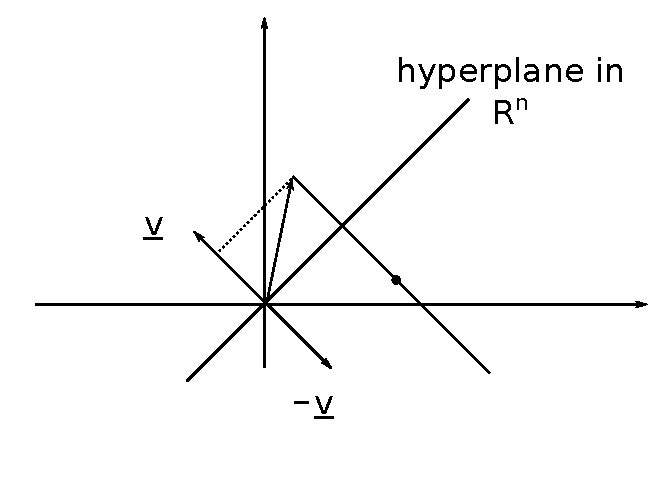
\includegraphics{img/06_transformation_P.pdf}
    \caption{Transformation $P$}
    \label{fig:transP}
  \end{center}
\end{figure}

Figure~\ref{fig:transP} illustrates the transformation.

with
\begin{align*}
  P^T P &= \left(I - \frac{2}{\underline{v}^T \underline{v}} \underline{v} \underline{v}^T\right) \left(I - \frac{2}{\underline{v}^T \underline{v}} \underline{v} \underline{v}^T\right) \\
    &= I - \frac{4}{\underline{v}^T \underline{v}} \underline{v} \underline{v}^T + \frac{4}{(\underline{v}^T \underline{v})^2} \underline{v} \underline{v}^T \underline{v} \underline{v}^T = I
\end{align*}

It holds that
\[ P \underline{v} = \left(I - \frac{2}{\underline{v}^T \underline{v}} \underline{v} \underline{v}^T\right) \underline{v} = \underline{v} - 2\underline{v} = -\underline{v} \]
and for $\underline{w}$ with $\underline{v}^T \underline{w} = 0$:
\[ P \underline{w} = \left(I - \frac{2}{\underline{v}^T \underline{v}} \underline{v} \underline{v}^T\right) \underline{w} = \underline{w} \]
For an arbitrary vector $\underline{x} \in \mathbb R^n$,
\[ \underline{x} = \frac{\underline{x}^T \underline{v}}{\underline{v}^T \underline{v}} \underline{v} + \frac{\underline{x}^T \underline{w}}{\underline{w}^T \underline{w}} = \underline{w} \]
and therefore
\[ P \underline{x} = \frac{\underline{x}^T \underline{v}}{\underline{v}^T \underline{v}} P \underline{v} + \frac{\underline{x}^T \underline{w}}{\underline{w}^T \underline{w}} P \underline{w} = - \frac{\underline{x}^T \underline{v}}{\underline{v}^T \underline{v}} \underline{v} + \frac{\underline{x}^T \underline{w}}{\underline{w}^T \underline{w}} \underline{w} \]

Hence, the Householder transformation $p$ describes a reflection of $\underline{x}$.
For the transformation of a given matrix $A$ is upper triangular form, we consider the transformation of the first column $\underline{a}$ of $A$ to a multiple of the first unit vector $\underline{e}$, i.e.
\[ P \underline{a} = \left(I - \frac{2}{\underline{v}^T \underline{v}} \underline{v} \underline{v}^T\right) \underline{a} \stackrel{!}{=} \alpha \underline{e} \]

First step, we want to find a transformation $P$ achieving the following transformation (as it turns out, this is the transformation $P$ from above)
\[
  P\left(\begin{pmatrix}
    * & \ldots & * \\
    \vdots &   & \vdots \\
    * & \ldots & *
  \end{pmatrix}\right)
  =
  \begin{pmatrix}
    * & * & \ldots & * \\
    0 & * &        & \vdots \\
    \vdots & \vdots & \ddots & \vdots \\
    0 & * & \ldots & *
  \end{pmatrix}
\]
The first columns are $\underline{a}$ and $\alpha \cdot \underline{e}$ respectively.

\textbf{Question:}
For which $\underline{v}$ does $P \underline{a} = \alpha \underline{e}$ hold?

\[ \underline{a} - \frac{2}{\underline{v}^T \underline{v}} \underline{v} \underline{v}^T \underline{a} = \underline{a} - 2 \frac{\underline{v}^T \underline{a}}{\underline{v}^T \underline{v}} \underline{v} \stackrel{!}{=} \alpha \underline{e} \]
i.e.
\[ \underline{v} = \gamma(\underline{a} - \alpha \underline{e}) \]

Because the definition of $P$ contains the normalization of $\underline{v}$, it can be chosen that
\[ \underline{v} = \underline{a} - \alpha \underline{e} \]
So, from
\begin{align*}
  \alpha \underline{e}
    &= P \underline{a} = \left(I - \frac{2}{\underline{v}^T \underline{v}} \underline{v} \underline{v}^T\right) \underline{a} \\
    &= \underline{a} - 2 \frac{\underline{v}^T \underline{a}}{\underline{v}^T \underline{v}} \underline{v} \\
    &= \underline{a} - 2 \frac{\underline{v}^T \underline{a}}{\underline{v}^T \underline{v}} (\underline{a} - \alpha \underline{e}) \\
    &= \left(1 - 2 \frac{\underline{v}^T \underline{a}}{\underline{v}^T \underline{v}}\right) \underline{a} + 2 \frac{\underline{v}^T \underline{a}}{\underline{v}^T \underline{v}} \alpha \underline{e}
\end{align*}
it follows that
\[ 2 \underline{v}^T \underline{a} = \underline{v}^T \underline{v} \]
With
\begin{align*}
  \underline{v}^T \underline{v}
    &= (\underline{a}^T - \alpha \underline{e}^T) (\underline{a} - \alpha \underline{e}) = \underline{a}^T \underline{a} - \alpha \underline{e}^T \underline{a} - \alpha \underline{a}^T \underline{e} + \alpha^2 \underline{e}^T \underline{e} \\
    &= \underline{a}^T \underline{a} - 2 \alpha a_{11} + \alpha^2
\end{align*}
and
\[ \underline{v}^T \underline{a} = (\underline{a}^T - \alpha \underline{e}) \underline{a} = \underline{a}^T \underline{a} - \alpha \underline{e}^T \underline{a} = \underline{a}^T \underline{a} - \alpha a_{11} \]
and
\[ 2 [\underline{a}^T \underline{a} - \alpha a_{11}] = 2 \underline{v}^T \underline{a} = \underline{v}^T \underline{v} = \underline{a}^T \underline{a} - 2 \alpha a_{11} + \alpha^2 \]
results in
\[ \alpha^2 = \underline{a}^T \underline{a} \]
To reduce the risk of decimal point cancellation
\[
  \alpha = \begin{cases}
    -\norm{a}_2 & a_{11} \geq 0 \\
    \norm{a}_2 & a_{11} < 0
  \end{cases}
\]

\textbf{Example:}
\[
  A = \begin{pmatrix}  2 & 1 & 0 \\ 1 & 4 & 1 \\ 0 & 1 & 2  \end{pmatrix}
  \qquad
  \underline{a} = \begin{pmatrix} 2 \\ 1 \\ 0 \end{pmatrix}
  \qquad
  \norm{a}_2 = \sqrt{5}
  \qquad
  \alpha = -\sqrt{5}
\] \[
  \underline{v} = \underline{a} - \alpha \underline{e} = \begin{pmatrix} 2 + \sqrt{5} \\ 1 \\ 0 \end{pmatrix},
  \underline{v}^T \underline{v} = 10 + 4 \sqrt{5}
\]

We call it $P_1$, because after the first column, it has to be applied iteratively.
\[
  P_1 = I - \frac{2}{\underline{v}^T \underline{v}} \underline{v} \underline{v}^T = \frac{1}{5 + 2\sqrt{5}}
  \begin{pmatrix}
    -4 - 2\sqrt{5} & -2-\sqrt{5} & 0 \\
    -2-\sqrt{5} & 4 + 2\sqrt{5} & 0 \\
    0 & 0 & 5 + 2\sqrt{5}
  \end{pmatrix}
\] \[
  P_1 A = \ldots = \frac{1}{5 + 2\sqrt{5}} \begin{pmatrix}
    -10 - 5 \sqrt{5} & -12 -6\sqrt{5} & -2-\sqrt{5} \\
    0 & 14 + 7\sqrt{5} & 4 + 2\sqrt{5} \\
    0 & 5 + 2\sqrt{5} & 10 + 4\sqrt{5}
  \end{pmatrix}
\]
Application to the first column of the lower matrix.
\[ \underline{a} = \begin{pmatrix} 0 \\ 14 + 7\sqrt{5} \\ 5 + 2\sqrt{5} \end{pmatrix} \]

\subsection{Givens rotation}
%
Especially for sparse matrices, the Givens rotation can help to eliminate specific entries.

\[ G = \begin{pmatrix} \alpha & -\beta \\ \beta & \alpha \end{pmatrix} \text{ with } \alpha^2 + \beta^2 = 1 \]
\[ G^T G = \begin{pmatrix} \alpha & \beta \\ -\beta & \alpha \end{pmatrix} \begin{pmatrix} \alpha & -\beta \\ \beta & \alpha \end{pmatrix} = \begin{pmatrix} \alpha^2 + \beta^2 & 0 \\ 0 & \alpha^2 + \beta^2 \end{pmatrix} = I \]
Transformation:
\[
  \begin{pmatrix}
    \alpha & -\beta \\
    \beta & \alpha
  \end{pmatrix} \begin{pmatrix}
    x \\ y
  \end{pmatrix}
  \stackrel{!}{=} \begin{pmatrix}
    \overline{x} \\ 0
  \end{pmatrix}
\]
\[ \beta x + \alpha y  = 0 \implies \alpha = \frac{x}{\sqrt{x^2 + y^2}}, \beta = -\frac{y}{\sqrt{x^2 + y^2}} \]

\textbf{Example:}
\[
  A = \begin{pmatrix} 2 & 1 & 0 \\ 1 & 4 & 1 \\ 0 & 1 & 2 \end{pmatrix}
  \qquad
  \underline{a} = \begin{pmatrix} 2 \\ 1 \end{pmatrix}
  \qquad
  x = 2, y = 1, \alpha = \frac2{\sqrt{5}}, \beta = -\frac1{\sqrt{5}}
\]
Rotation in the $x_1$-$x_2$-plane:
\[ G_1 = \frac{1}{\sqrt{5}} \begin{pmatrix} 2 & 1 & 0 \\ -1 & 2 & 0 \\ 0 & 0 & -\sqrt{5} \end{pmatrix} \]
\[ G_1 A = \frac{1}{\sqrt{5}} \begin{pmatrix} 5 & 6 & 1 \\ 0 & 7 & 2 \\ 0 & \sqrt{5} & 2 \sqrt{5} \end{pmatrix} \]
\[ \underline{a} = \frac{1}{\sqrt{5}} \begin{pmatrix} 7 \\ \sqrt{5} \end{pmatrix}, x = \frac{7}{\sqrt{5}}, y = 1, \alpha = \frac{7}{\sqrt{54}}, \beta = -\frac{\sqrt{5}}{\sqrt{54}} \]
\[ G_2 = \frac{1}{\sqrt{54}} \begin{pmatrix} \sqrt{54} & 0 & 0 \\ 0 & 7 & \sqrt{5} \\ 0 & -\sqrt{5} & 7 \end{pmatrix} \]
\[ R = G_2 G_1 A = \ldots = \frac{1}{\sqrt{220}} \begin{pmatrix} 5\sqrt{54} & 6\sqrt{54} & \sqrt{54} \\ 0 & 54 & 24 \\ 0 & 0 & 12 \sqrt{15} \end{pmatrix} \]
$\to A = QR$ with $Q = (G_2 G_1)^T$.

\subsection{Stationary iteration methods}

Stationary refers to: $x^{k+1} = T(x^k) \text{ with } T \neq T^k$

% TODO: this equation should be 4.1
\begin{align}
  A \underline{x} &= \underline{f} \text{ with } \underline{x} = \underline{x} + \alpha B^{-1} (A\underline{x} - \underline{f}) \label{eq:eq41}
\end{align}

For a regular matrix $B \in \mathbb R^{n\times n}$ and a positive real parameter $\alpha \in \mathbb R$ is the solution of the linear equation system~\ref{eq:eq41} equivalent to the solution of the fixed point equation~\ref{eq:eq42}.
\begin{align}
  \underline{x} &= \underline{x} - \alpha B^{-1} (A\underline{x} - f) \label{eq:eq42}% TODO: this equation should be 4.2
\end{align}

This representation gives rise to the iteration process~\ref{eq:eq43}
\[ \underline{x}^{k+1} \coloneqq \underline{x}^k - \alpha B^{-1} (A \underline{x}^k - \underline{f}) = (I - \alpha B^{-1} A) \underline{x}^k + \alpha B^{-1} \underline{f} \label{eq:eq43} \]
(with an arbitrary chosen initial approximation $\underline{x} \in \mathbb R^n$) for $k = 0, 1, 2, \ldots$.
The convergence of the process~\ref{eq:eq43} follows from Banach's fixed point theorem.

\begin{theorem}
  The iteration matrix of the iteration process~\ref{eq:eq43} is a contraction, hence it holds that
  \begin{align} \norm{I - \alpha B^{-1} A}_M \leq q < 1 \label{eq:eq44} \end{align}
  in a vector norm $\norm{\cdot}_V$ compatible to matrix norm $\norm{\cdot}_M$.
  Then iteration process~\ref{eq:eq43} converges against a uniquely defined solution $\underline{x} = A^{-1} \underline{f}$ of the linear equation system~\ref{eq:eq41} and the following a priori error estimate is given:
  \begin{align} \norm{\underline{x}^{k+1} - \underline{x}}_V \leq \frac{q^{k+1}}{1 - q} \norm{\underline{x}^1 - \underline{x}^0}_V \label{eq:eq45} \end{align}
  as well as the posteriori error estimate
  \begin{align} \norm{\underline{x}^{k+1} - \underline{x}}_V \leq \frac{q}{1 - q} \norm{\underline{x}^{k+1} - \underline{x}^k}_V \label{eq:eq46} \end{align}
\end{theorem}

\begin{proof}
  The exact solution $\underline{x} = A^{-1} \underline{f}$ of the linear equation system~\ref{eq:eq41}
  is the solution of the fixed point equation~\ref{eq:eq42}. Then it follows that,
  \begin{align*}
    \norm{\underline{x}^{k+1} - \underline{x}}_V &= \norm{(I - \alpha B^{-1} A)(\underline{x}^k \underline{x})}_V \\
      &\leq \norm{I - \alpha B^{-1} A}_M \norm{\underline{x}^k - \underline{x}} \\
      &\leq q \norm{\underline{x}^k - \underline{x}}
  \end{align*}
  and by repetitive application, we get:
  \begin{align*} \norm{\underline{x}^{k+1} - \underline{x}} &\leq q^{k+1} \norm{\underline{x}^0 - \underline{x}} \to 0 \text{ for } k \to \infty \end{align*}
  because $q < 1$ for every arbitrary initial approximation $\underline{x}^0 \in \mathbb R^n$.

  By the triangle inequality
  \[
    \norm{\underline{x}^{k+1} - \underline{x}}_V
    \leq q \norm{\underline{x}^k - \underline{x}}_V
    \leq q \left(\norm{x^k - x^{k+1}}_V + \norm{\underline{x}^{k+1} - \underline{x}}_V\right)
  \] \[
    \iff (1 - q) \norm{x^{k+1} - x}_V \leq q \norm{x^{k+1} - x^k}_V
  \]
  the a posteriori error estimate~\ref{eq:eq46} follows.

  From,
  \[ \norm{\underline{x}^{k+1} - \underline{x}}_V \leq q^k \norm{\underline{x}^1 - \underline{x}}_V \]
  and by the a posteriori error estimate for $k=0$,
  \[ \norm{x^1 - \underline{x}}_V \leq \frac{q}{1 - q} \norm{\underline{x}^1 - \underline{x}^0}_V \]
  the a priori error estimate can be derived.
\end{proof}

An arbitrary matrix $A \in \mathbb R^{n \times n}$ is representable as
\begin{align} A &= L + D + R \label{eq:eq47} \end{align}
where $L$ refers to the lower triangular matrix slice, $D$ to the diagonal values and $R$ to the upper triangular matrix slice.
\[
  L = \begin{pmatrix}
    0      &        &           & 0 \\
    a_{21} & 0      &           & \\
    \vdots &        & \ddots    & \\
    a_{n1} & \ldots & a_{n,n-1} & 0
  \end{pmatrix}
  \qquad
  R = \begin{pmatrix}
    0      & a_{12} & \ldots    & a_{1n} \\
           & \ddots &           & \vdots \\
           &        & \ddots    & a_{n-1,n} \\
    0      &        &           & 0
  \end{pmatrix}
  \qquad
  D = \begin{pmatrix}
    a_{11} &        & 0       & \\
           & a_{22} &         & \\
           &        & \ddots  & \\
           &        &         & a_{nn}
  \end{pmatrix}
\]
Because of invertibility of $A$ we can (without loss of generality) assume the invertability of diagonal matrix $D$.

Then the linear equation system~\ref{eq:eq41} is equivalent to fixed point equation:
\[ D \underline{x} = f - (L + R) \underline{x} \]
resulting in the Jacobi method (\enquote{complete step procedure})
\begin{align} \underline{x}^{k+1} = D^{-1}(f - (L + R) \underline{x}^k) = \underline{x}^k - D^{-1} (A\underline{x}^k - f) \label{eq:eq48} \end{align}

\dateref{2017/12/06}

Can we apply Equation~\ref{eq:eq41} to this process?

\subsection{Jacobi method}
\index{Jacobi method}

Algorithm:
\begin{enumerate}
  \item Let $\underline{x}^0 \in \mathbb R^n$ an arbitrary initial approximation.
  \item For $k = 0,1,2,\ldots$
    \begin{enumerate}
       \item compute $\underline{r}^k = A \underline{x}^k - \underline{f}, g_k = (\underline{r}^k, \underline{r}^k) = \norm{\underline{r}^k}_2^2$
     \end{enumerate}
  \item If $g_k \leq \varepsilon^2 g_0$ with given error precision $\varepsilon$ is achieved, terminate.
  \item $x_i^{k+1} = \frac{1}{a_{ii}} \left[f_i - \sum_{j=1}^{i-1} a_{ij} x_j^k - \sum_{j=1+1}^n a_{ij} x_j^k\right]$ for $i=1,\ldots,n$
\end{enumerate}

\begin{definition} % Satz 4.2
  \label{satz42}
  For matrix $A$, the \emph{strong row sum criterion} is defined as
  \[ \max_{i=1,\ldots,n} \sum_{\substack{j=1 \\ j \neq i}}^n \frac{\card{a_{ij}}}{\card{a_{ii}}} \leq q < 1 \]
  Then the Jacobi method (equation~\ref{eq:eq48}) converges for any arbitrary initial approximation $\underline{x}^0$.
\end{definition}

\begin{proof}
  \begin{itemize}
    \item $\norm{\cdot}_V = \norm{\cdot}_{\infty}$ is compatible with $\norm{\cdot}_M = \norm{\cdot}_\infty$ where $\norm{\cdot}_\infty$ is the row sum norm.
    \item Iteration matrix
      \[ \norm{\underbrace{I - D^{-1} A}_{\substack{0 \text{ at diagonal} \\ \frac{a_{ij}}{a_{ii}} \text{ otherwise}}}}_\infty = \max_{i=1,\ldots,n} \sum_{\substack{i=1 \\ j\neq 1}}^n \frac{\card{a_{ij}}}{\card{a_{ii}}} \leq q < 1 \]
      Hence, by Equation~\ref{eq:eq41}, convergence of the Jacobi method is given.
  \end{itemize}
\end{proof}

Starting from Equation~\ref{eq:eq47}, the linear equation system~\ref{eq:eq41} is equivalent to the fixed point equation
\[ (D + L) \underline{x} = \underline{f} - R \underline{x} \]
resulting in the derivation of the forwarding\footnote{Using forward insertion.} Gauss-Seidel method (\enquote{single step method})
\begin{align}
  \underline{x}^{k+1} &= (D + L)^{-1} \left[\underline{f} - R \underline{x}^k\right] = \underline{x}^k - (D + L)^{-1} [A \underline{x}^k - f] \\
    &= (D + L)^{-1} R \underline{x}^k + (D + L)^{-1} \underline{f} \label{eq:eq49}
\end{align}

\[ (D + L) \underline{x}^{k+1} = \underline{b} \]
\[
  \begin{pmatrix}
    a_{11} &        &        & \\
    a_{21} & a_{22} &        & \\
    \vdots &        & \ddots & \\
    a_{n1} & \ldots &        & a_{nn}
  \end{pmatrix} \cdot
  \begin{pmatrix}
    x_1^{k+1} \\ x_2^{k+1} \\ \vdots \\ x_n^{k+1}
  \end{pmatrix}
  =
  \begin{pmatrix} b_1 \\ b_2 \\ \vdots \\ b_n \end{pmatrix}
  \leadsto
  \substack{
    x_1^{k+1} = \frac{b_{{1}}}{a_{11}} \\ \\
    x_2^{k+1} = \frac{1}{a_{22}} (b_2 - a_{21} x_1^{k+1}) \\
    \vdots
  }
\]

\subsection{Forwarding Gauss-Seidel method}

\begin{enumerate}
  \item Let $\underline{x}^0 \in \mathbb R^n$ be an arbitrary initial approximation.
  \item For $k = 0, 1, 2, \ldots$, determine
    \begin{enumerate}
      \item $\underline{r}^k = A \underline{x}^k - f, g_k = (\underline{r}^k, \underline{r}^k) = \norm{\underline{r}^k}_2^2$
    \end{enumerate}
  \item If $g_k \leq \varepsilon^2 g_0$ for given $\varepsilon$, terminate
  \item $x_i^{k+1} = \frac{1}{a_{ii}} \left[f_i - \sum_{j=1}^{i-1} a_{ij} x_j^{k+1} - \sum_{j=i+1}^n a_{ij} x_j^k\right]$ for $i = 1, \ldots, n$
\end{enumerate}

\begin{theorem} % Satz 4.3
  \label{satz43}
  For matrix $A$, let the strong row sum criterion be satisfied (compare with Theorem~\ref{satz42}).
  Then the Gauss-Seidel method~\ref{eq:eq49} converges for an arbitrary initial approximation $\underline{x}^0$.
\end{theorem}
\begin{proof}
  Show $\norm{(D+L)^{-1} R}_{\infty} \leq q < 1$ (then the statement from Equation~\ref{eq:eq41} follows).

  For arbitrary $\underline{y} \in \mathbb R^n$, consider the linear equation system
  \[ (D + L) \underline{z} = R \underline{y} \]
  Then it holds that
  \[ z_1 = \frac{1}{a_{11}} \sum_{j=2}^n a_{1j} y_j \]
  and therefore
  \[ \card{z_1} \leq \sum_{j=2}^n \frac{\card{a_{1j}}}{\card{a_{11}}} \card{y_{j}} \leq \max_{l=1,\ldots,n} \card{y_l} \sum_{j=2}^n \frac{\card{a_{1j}}}{\card{a_{1i}}} \leq q \norm{y}_\infty \]
  Hence, it holds that
  \[ \card{z_l} \leq q \norm{y}_{\infty} < \norm{y}_{\infty} \text{ for } l=1,\ldots,k-1 \]
  Then it follows that
  \begin{align*}
    \norm{z_k} &= \frac{1}{\card{a_{kk}}} \card{-\sum_{l=1}^{k-1} a_{kl} z_l + \sum_{l=k+1}^n a_{kl} y_l} \\
      &\leq \frac{1}{\card{a_{kk}}} \left[ \max_{l=1,\ldots,k-1}] \card{z_l} \sum_{l=1}^{k-1} \card{a_{kl}} + \max_{l=k+1,\ldots,n} \card{y_l} \sum_{l=k-1}^n \card{a_{kl}}\right] \\
      &\leq \norm{y}_{\infty} \sum_{l=1}^n \frac{\card{a_{kl}}}{\card{a_{kk}}} \leq q \norm{y}_{\infty}
  \end{align*}
  for $k=2,\ldots,n$ and therefore it holds that
  \[ \norm{(D+L)^{-1} R \underline{y}}_{\infty} = \norm{z}_{\infty} \leq q \norm{y}_{\infty} \]
  Because the row sum norm is induced by the maximum norm, it follows that
  \[ \norm{(D+L)^{-1} R}_{\infty} = \sup_{\substack{y \in \mathbb R^n \\ y \neq 0}} \frac{\norm{(D+L)^{-1} Ry}_{\infty}}{\norm{y}_{\infty}} \leq q < 1 \]
  The convergence of the Gauss-Seidel method (acc. to Equation~\ref{eq:eq41}) follows.
\end{proof}

\dateref{2017/12/11}

\subsection{Revision of Jacobi and Gauss-Seidel methods}

\[ A \underline{x} = \underline{f} \]
For $i = 1,\ldots,n$,
\[ \hat x_i^{k+1} = \frac{1}{a_{ii}} \left[ f_i - \sum_{\substack{j=1 \\ j \neq i}}^n a_{ij} x_j^k \right] \]
\[ x_i^{k+1} = (1 - \omega) x_i^k + \hat x_i^{k+1} \]
where $\omega$ is called relaxation parameter with $\omega \in (0,1]$.
\begin{align*}
  x_i^{k+1} &= (1 - \omega) x_i^k + \omega \hat x_i^{k+1} \\
    &= (1 - \omega) x_i^k + \omega \frac{1}{a_{ii}} \left[f_i - \sum_{\substack{j=1 \\ j \neq i}}^n a_{ij} x_j^k\right] \\
    &= x_i^k + \omega \frac{1}{a_{ii}} \left[ f_i - \sum_{j=1}^n a_{ij} x_j^k \right] \\
    &= x_i^k - \omega \frac{1}{a_{ii}} \left[\sum_{j=1}^{n} a_{ij} x_j^k - f_i\right] \qquad i = 1,\ldots,n \\
  \underline{x}^{k+1} &= \underline{x}^k - \omega D^{-1} (A \underline{x}^k - \underline{f})
\end{align*}

This method is called \emph{Richardson Iteration} or \emph{$\omega$-Jacobi method}.

Another interpretation is given with:
\begin{align*}
  A \underline{x} &= \underline{f} \\
  \iff \underline{0} &= A \underline{x} - \underline{f} \\
  \underline{0} &= -gB^{-1} (A \underline{x} - \underline{f}) \\
  \underline{x} &= \underline{x} - gB^{-1} (A \underline{x} - \underline{f})
\end{align*}
Where $g \neq 0$ and $B$ is regular. Fixed point equation.

Richardson Iteration:
\[ \underline{x}^{k+1} = x^k - gB^{-1} (A \underline{x}^k - \underline{f}) \]
For example $b = \diag(A), \gamma = w$.

Gauss-Seidel method: for $i = 1, \ldots, n$,
\begin{align*}
  \hat x_i^{k+1} &= \frac{1}{a_{ii}} \left[f_i - \sum_{j=1}^{i-1} a_{ij} x_j^{k+1} - \sum_{j=i+1}^n a_{ij} x_j^k\right] \\
  x_i^{k+1} &= (1 - \omega) x_i^k + \omega \hat x_i^{k+1} \\
            &= (1 - \omega) x_i^k + \frac{\omega}{a_{ii}} \left[ f_i - \sum_{j=1}^{i-1} a_{ij} x_j^{k+1} - \sum_{j=i+1}^n a_{ij} x_j^k\right] \\
  x_i^{k+1} &= x_i^k + \frac{\omega}{a_{ii}} \left[f_i - \sum_{j=i}^n a_{ij} x_j^k\right] - \frac{\omega}{a_{ii}} \sum_{j=1}^{i-1} a_{ij} x_j^{k+1} \\
  a_{ii} x_i^{k+1} + \omega \sum_{j=1}^{i-1} a_{ij} x_j^{k+1} &= a_{ii} x_i^k + \omega \left[f_i - \sum_{j=i}^n a_{ij} x_j^k\right] \\
\intertext{Consider matrix $A = L + D + R$ where $L$ is a lower triangular matrix, $D$ only contains diagonal elements and $R$ is the right upper triangular matrix. Then,}
  D \underline{x}^{k+1} + \omega L \underline{x}^{k+1} &= D \underline{x}^k + \omega \left[\underline{f} - \omega (D + R) \underline{x}^k\right]
    &= D \underline{x}^k + \omega \left[ \underline{f} - A \underline{x}^k + L \underline{x}^k \right] \\
  (D + \omega L) \underline{x}^{k+1} &= (D + \omega L) \underline{x}^k - \omega (A \underline{x}^k - \underline{f})
\end{align*}

Successive Over-Relaxation (SOR) method:
\[ \implies \underline{x}^{k+1} = \underline{x}^k - \omega (D + \omega L)^{-1} (A \underline{x}^k - \underline{f}) \]

\begin{theorem}
  Ostrowski, 1947

  Let $A$ be a symmetric matrix and be positive definite. Then the SOR method converges
  if and only if $\omega \in (0,2)$.
\end{theorem}
\begin{proof}
  To be done in the practicals.
\end{proof}

Ostrowski's theorem applied to $\omega=1$ shows the convergence of the Gauss-Seidel method for symmetric, positive definite matrices $A$.

But one problem occurs.
Even for a symmetric matrix the recursion matrix won't become symmetric:
$g = \omega$, $B = D + \omega L$, $A = A^T \implies B \neq B^T$.

Thus, we want to derive a symmetric method.

SOR (in forwards direction\footnote{Corresponds to \enquote{top to bottom} in the matrix}:
\[ \underline{x}^{k+1} = \underline{x}^{k+1} - \omega(D + \omega L)^{-1} \left[A \underline{x}^k - \underline{f}\right] \]

Let us consider again,
\[ x_i^{k+1} = (1 - \omega) x_i^k + \frac{\omega}{a_{ii}} \left[ f_i - \sum_{j=1}^{i-1} a_{ij} x_j^{k+1} - \sum_{j=i+1}^n a_{ij} x_j^k\right] \]
but we replace some $k$ and $k+1$:
\[ x_i^{k+1} = (1 - \omega) x_i^k + \frac{\omega}{a_{ii}} \left[ f_i - \sum_{j=1}^{i-1} a_{ij} x_j^{k} - \sum_{j=i+1}^n a_{ij} x_j^{k+1}\right] \]

We get some SOR in backwards direction:
\[ \underline{x}^{k+1} = \underline{x}^{k+1} - \omega(D + \omega R)^{-1} \left[A \underline{x}^k - \underline{f}\right] \]

Now we combine these two SOR variants.
\begin{align*}
  \underline{x}^{k+\frac12} &= \underline{x}^k - \omega (D + \omega L)^{-1} \left[ A \underline{x}^k - \underline{f} \right] \\
  \underline{x}^{k+1} &= \underline{x}^{k+\frac12} - \omega (D + \omega R)^{-1} \left[ A \underline{x}^{k+\frac12} - \underline{f} \right] \\
    & \ldots \\
  \underline{x}^{k+1} &= \underline{x}^k - \underbrace{\omega (2 - \omega)}_{g} \underbrace{(D + \omega R)^{-1} D (D + \omega L)^{-1}}_{B = B^T > 0 \text{ for } A = A^T > 0} \left[ A \underline{x}^k - \underline{f} \right]
\end{align*}

Symmetric Successive OverRelaxation (ISSOR method):
\[ A = A^T > 0 \implies \text{ convergence } \iff \omega \in (0,2) \]

$B$ acts as a precondition.

All these methods can be considered as Richardson iteration.

\subsection{Richardson iteration, Methods of single iteration}
%
\[ \underline{x}^{k+1} = \underline{x}^k - \alpha (A \underline{x}^k - \underline{f}) \]
$\alpha$ is constant and therefore this is called a stationary method.

\[ A = A^T > 0 \qquad \norm{\underline{x}^{k+1} - \underline{x}}_V \leq \underline{q} \norm{\underline{x}^k - \underline{x}}_V \qquad q < 1 \]
\begin{align*}
  \underline{x}^{k+1} &= \underline{x}^k - \alpha (A \underline{x}^k - \underline{f}) \\
  \underline{x}       &= \underline{x} - \alpha (A \underline{x} - \underline{f}) \\
  \underline{x}^{k+1} - \underline{x} &= \underbrace{(I - \alpha A)}_{M} (\underline{x}^k - \underline{x})
\end{align*}

\[ \norm{\cdot}_V = \norm{\cdot}_2 \]
\begin{align*}
  \norm{\underline{e}^{k+1}}_2^2 &= \norm{(I - \alpha A) \underline{e}^k}_2^2 = \left((I - \alpha A) \underline{e}^k, (I - \alpha A) \underline{e}^k\right) \\
    &= \norm{g^k}_2^2 - 2 \alpha \underbrace{(A \underline{e}^k, \underline{e}^k)}_{\geq c_1^A \norm{\underline{e}^k}_2^2} + \alpha^2 \underbrace{(A \underline{e}^k, A \underline{e}^k)}_{\leq (c_2^A)^2 \norm{\underline{e}^k}_2^2} \\
    &\leq \underbrace{(1 - 2 \alpha c_1^A + (c_2^A)^2)}_{< 1} \norm{\underline{e}^k}_2^2
\end{align*}
when is it minimal for $\alpha^*$? It depends on $c_1^A$ and $c_2^A$.

So how do we choose $\alpha^*$ and $\norm{\cdot}_V$. For the latter we can use $A = A^T > 0$ or $A \neq A^T$ indefinit.
Those lead us to the gradient methods and orthogonalization/CG method.

% projects for the practicals:
% - Chebyshev interpolation (convergence study, by incrementing the number of supporting points, etc)
% - L2 projection, uniform mesh (convergence study)
% - L2 projection, non-uniform mesh (convergence study)
% - Gauss quadrature, error
% - Weighted integration
% - CG method, (mass matrix:) M_h \underline{u} = \underline{f}, uniform mesh, diagonal-VK
% - CG method, M_h \underline{u} = \underline{f}, diagonal-VK, non-uniform mesh
% - nonlinear scalar equations (Newton)

\dateref{2017/12/13}

\section{Gradient methods}

Let $A \in \mathbb R^{n\times n}$ be regular, $\underline{x} = A^{-1} \underline{f}$ be the solution of Equation~\ref{eq:eq41} ($A \underline{x} = \underline{f}$).
Additionally, we assume $A$ is symmetric and positive definite.

Now we reformulate the problem as an optimization problem. Consider,
\[ F: \mathbb R^n \to \mathbb R \]
\[ F(\underline{z}) = \norm{\underline{z} - \underline{x}}_A^2 = (A(\underline{z} - \underline{x}), \underline{z} - \underline{x}) = (A \underline{z}, \underline{z}) - 2 (\underbrace{A \underline{x}}_{= \underline{f}}, \underline{z}) + \norm{\underline{x}}_A^2 \]
with the vector norm $\norm{\cdot}_A$ induced by $A$.

For the solution $\underline{x} = A^{-1} f$ of Equation~\ref{eq:eq41} it holds that,
\[ 0 = F(\underline{x}) = \min_{\underline{z} \in \mathbb R^n} F(\underline{z}) \]

Let $\underline{x}^k$ be the given approximate solution and $\underline{r}^k = A \underline{x}^k - \underline{f}$ is the corresponding residue.
We consider a new approach with approximate solution,
\[ \underline{x}^{k+1} = \underline{x}^k + \alpha_k f^k \]
where $\underline{p}^k$ (the direction of search) is chosen in direction of the negative gradient.
\[ -\left(\left.\nabla F(\underline{z})\right|_{\underline{z} = \underline{x}^k}\right) = -\left(\left.2 (A\underline{z} - \underline{f})\right|_{\underline{z} = \underline{x}^k}\right) = 2(A \underline{x}^k - \underline{f}) = -2\underline{r}^k \]
By neglecting the factor $2$ we get,
\[ \underline{x}^{k+1} = \underline{x}^k - \alpha_k \underline{r}^k \]
The real parameter $\alpha_k$ is chosen such that $F$ is minimal:
\[ F(\underline{x}^{k+1}) = F\left(\underline{x}^k - \alpha_k \underline{r}^k\right) \stackrel!= \min_{\alpha \in \mathbb R} F\left(\underline{x}^k - \alpha \underline{r}^k\right) \]

Because
\begin{align*}
  F(\underline{x}^k - \alpha \underline{r}^k)
    &= \norm{\underline{x}^k - \alpha \underline{r}^k - \underline{x}}_A^2 \\
    &= (A(\underline{x}^k - \alpha \underline{r}^k - \underline{x}), \underline{x}^k - \alpha \underline{r}^k - \underline{x}) \\
    &= (A(\underline{x}^k - \underline{x}), \underline{x}^k - \underline{x}) - 2 \alpha (A(\underline{x}^k - \underline{x}), \underline{r}^k) + \alpha^2 (A \underline{r}^k, \underline{r}^k) \\
    &= F(\underline{x}^k) - 2\alpha (\underline{r}^k, \underline{r}^k) + \alpha^2 (A \underline{r}^k, \underline{r}^k)
\end{align*}
the minimum is assumed for
\[ \alpha_k = \frac{(\underline{r}^k, \underline{r}^k)}{(A\underline{r}^k, \underline{r}^k)} \]
\index{Gradient method of steepest decent}
The resulting method is called \emph{gradient method of steepest decent}.

Algorithm:
\begin{enumerate}
  \item Given initial approximation $\underline{x}^0$ (arbitrary), $\underline{r}^0 = A \underline{x}^0 - \underline{f}$
  \item For $k=0,1,2,\ldots$
    \begin{enumerate}
      \item $g_k = (\underline r^k, \underline r^k) = \norm{\underline r^k}_2^2$
    \end{enumerate}
  \item Terminate if $g_k \leq \varepsilon^2 g_0$ with given error precision $\varepsilon$.
  \item $\underline v^k = A \underline r^k, \alpha_k = \frac{(\underline r^k, \underline r^k)}{(\underline v^k, \underline r^k)}, \underline x^{k+1} = \underline x^k - \alpha_k \underline r^k$, $\underline r^{k+1} = \underline r^k - \alpha_k \underline v^k$
\end{enumerate}

\begin{theorem}
  Let $A$ be symmetric and positive definite. Furthermore it holds that
  \[ (A \underline{x}, \underline{x}) \geq c_1^A \norm{\underline{x}}_2^2 \qquad \norm{A \underline{x}}_2 \leq c_2^A \norm{\underline x}_2  \]
  for all $\underline{x} \in \mathbb R^n$. Then the gradient method of steepest decent converges towards
  \[ \norm{\underline{x}^{k+1} - \underline{x}}_A^2 \leq \left(1 - \left(\frac{c_1^A}{c_2^A}\right)^2\right)^{k+1} \norm{\underline x_0 - \underline x}_A^2 \]
\end{theorem}

In case if $A$ is not symmetrically positive definite,
\begin{itemize}
  \item 
    \[ \tilde F(z) = \norm{z - \underline{x}}_{A^T A}^{2} \]
    where $A^T A$ is symmetrically positive definite.
    \[ \implies \underline p^k = \left. -\nabla \tilde F(z) \right|_{z = \underline{x}^k} = -2 A^T \underline{r}^k \]
    $\alpha_k$ such that
    \[ \tilde F(\underline{x}^{k+1}) = \tilde F(\underline{x}^k - \alpha_k A^T \underline{r}^k) \stackrel!= \min_{\alpha \in \mathbb R} \tilde F(x^k - \alpha A^T \underline{r}^k) \]
    \[ \implies \alpha_k = \frac{(A^T \underline r^k, A^T \underline r^k)}{(AA^T \underline r^k, AA^T \underline r^k)} \]
  \item
    Gradient method of minimal defect

    The direction of search is the negative residue
    \[ \underline x^{k+1} = \underline x^k - \alpha_k \underline r^k \]
    where $\alpha_k$ such that
    \[ \tilde F(\underline x^{k+1}) = \tilde F(\underline x^k - \alpha_k \underline r^k) \stackrel!= \min_{\alpha \in \mathbb R} \tilde F(\underline{x}^k - \alpha \underline{r}^k) \]
    \[ \implies \alpha_k = \frac{(A \underline r^k, \underline r^k)}{(A \underline r^k, A \underline r^k)} \]
    Convergence behavior is analogously to $\norm{\cdot}_{A^TA}$ instead of $\norm{\cdot}_A$.
\end{itemize}

\begin{example}
  Gradient method of steepest decent for
  \[ \begin{pmatrix} 2 & 1 \\ 1 & 2 \end{pmatrix} \begin{pmatrix} x_1 \\ x_2 \end{pmatrix} = \begin{pmatrix} 5 \\ 4 \end{pmatrix} \text{ with initial value } \underline x^0 = \begin{pmatrix} 0 \\ 0 \end{pmatrix} \]
  \[ \underline r^0 = A \underline x^0 - f = \begin{pmatrix} -5 \\ -4 \end{pmatrix}, \alpha_0 = \frac{(\underline{r}^0, \underline{r}^0)}{(A \underline{r}^0, \underline{r}^0)} = \frac{41}{122} \]
  \[ \underline x^1 = \underline x^0 - \alpha_0 \underline r^0 \approx \begin{pmatrix} 1.680 \\ 1.344 \end{pmatrix} \]
  \begin{table}
    \begin{tabular}{cccc}
      $k$ & $x_1^k$ & $x_2^k$ & $F(x^k)$ \\
    \hline
      0 & 0 & 0 & 14 \\
      1 & 1.680 & 1.344 & $2.213 \cdot 10^{-1}$ \\
      2 & 1.968 & 0.984 & $3.499 \cdot 10^{-3}$ \\
      3 & 1.995 & 1.005 & $5.530 \cdot 10^{-5}$ \\
    \end{tabular}
  \end{table}
  Exact solution: $\underline x = \begin{pmatrix} 2 \\ 1 \end{pmatrix}$.
  \[ F(\underline z) = \left(\begin{pmatrix} 2 & 1 \\ 1 & 2 \end{pmatrix} \begin{pmatrix} z_1 - 2 \\ z_2 - 1 \end{pmatrix}, \begin{pmatrix} z_1 - 2 \\ z_2 - 1 \end{pmatrix}\right) \]
  \[ \implies \underline r^2 \approx \begin{pmatrix} -0.08 \\ -0.064 \end{pmatrix} \left\| \begin{pmatrix} -5 \\ -4 \end{pmatrix} = \underline r^0\right. \]
\end{example}

\begin{figure}[!h]
  \begin{center}
    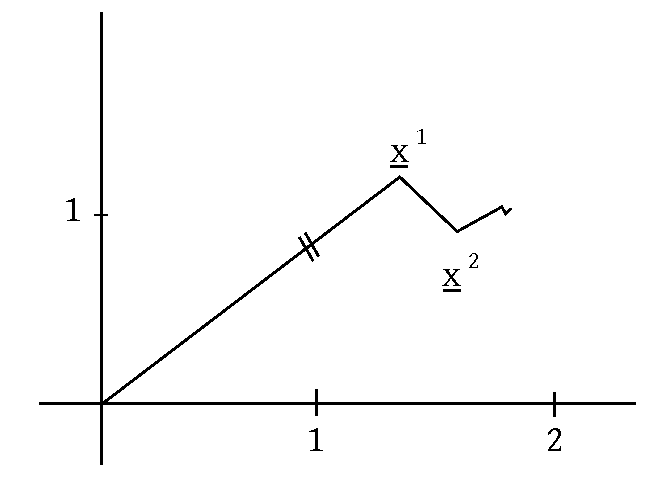
\includegraphics{img/gradient_method_search_direction.pdf}
    \caption{Gradient method search direction}
    \label{img:searchdir}
  \end{center}
\end{figure}
Advantage of the gradient method:
\begin{quote}
  Parallel oder almost parallel search directions can be traversed multiple times in one iteration.
  Compare with Figure~\ref{img:searchdir}.
\end{quote}
This motivates the \emph{orthogonalization of search directions}.

\dateref{2018/01/08}

\subsection[Conjugate gradient method]{Conjugate Gradient method, CG method}

\textbf{Assumption:} $A = A^T$, symmetrical and positive definite

A system of linear independent vectors $\left\{\underline{p}^k\right\}_{k=0}^{n-1}$ is called
\emph{A-orthogonal} or \emph{conjugated}, if
\[ (A\underline{p}^k, \underline{p}^l) = 0 \text{ for } k,l=0,\ldots,n-1 \text{ with } k\neq l \text{ and} \]
\[ (A \underline{p}^k, \underline{p}^k) > 0 \text{ for } k = 0,\ldots,n-1 \]

For linear independent $\left\{\underline{w}^k\right\}_{k=0}^{n-1}$, using the Gram-Schmidt orthogonalization method,
we can construct a system of $A$-orthogonal vectors $\left\{\underline{p}^k\right\}_{k=0}^{n-1}$.

% TODO stylize algorithm
% Construction of A-orthogonal vectors
\begin{itemize}
  \item Let $\underline{p}^0 \coloneqq \underline{w}^0$
  \item For $k=0,\ldots,n-2$ compute
    \[ \underline{p}^{k+1} \coloneqq \underline{w}^{k+1} - \sum_{l=0}^k \beta_{kl} \underline{p}^l \]
    with
    \[ \beta_{kl} = \frac{(A \underline{w}^{k+1}, \underline{p}^l)}{(A \underline{p}^l, \underline{p}^l)} \]
\end{itemize}

In the 2D-case (hence, if $n=2$), then the ideal situation would be to make one step ahead and
the next orthogonal step leads us directly to the solution.

We insert our solution approach:
\[ \underline{x} = \underline{x}^0 - \sum_{l=0}^{n-1} \alpha_l \underline{p}^l \]
into the linear equation system $A \underline{x} = \underline{f}$ results in
\[ A \underline{x} = A \underline{x}^0 - \sum_{l=0}^{n-1} \alpha_l A \underline{p}^l = \underline{f} \]
\[ \implies (A \underline{x}, \underline{p}^k) = (A \underline{x}^0, p^k) - \sum_{l=0}^{n-1} \alpha_l (A \underline{p}^l, \underline{p}^k) = (\underline{f}, \underline{p}^k) \]
for $k = 0, \ldots, n-1$.
Here $(A \underline{p}^l, \underline{p}^k) = 0$ if $l \neq k$ because $\left\{\underline{p}^k\right\}_{k=0}^{n-1}$ is $A$-orthogonal.
Hence,
\[ \implies \alpha_k = \frac{(A \underline{x}^0 - f, \underline{p}^k)}{(A \underline{p}^k, \underline{p}^k)} \]
for $k = 0, \ldots, n-1$.

For approximative solution
\[ \underline{x}^{k+1} = \underline{x}^0 - \sum_{l=0}^{k} \alpha_l \underline{p}^l = \underline{x}^0 - \sum_{l=0}^{k-1} \alpha_l \underline{p}^l - \alpha_k \underline{p}^k = \underline{x}^k - \alpha_k \underline{p}^k \]
is the associated residue given by
\[ \underline{r}^{k+1} = A \underline{x}^{k+1} - f = A \underline{x}^0 - \sum_{l=0}^k \alpha_l A \underline{p}^l - f = A \underline{x}^k - f - \alpha_k A \underline{p}^k = \underline{r}^k - \alpha_k A \underline{p}^k \]
Because $(A \underline{p}^l, \underline{p}^k) = 0$ for $k \neq l$, it follows that
\[ \left(A \underline{x}^0 - f, \underline{p}^k\right) = \left(A \underline{x}^0 - \sum_{l=0}^{k-1} \alpha_l A \underline{p}^l - f, \underline{p}^k\right) = (\underline{r}^k, \underline{p}^k) \]
and therefore
\[ \alpha_k = \frac{(\underline{r}^k, \underline{p}^k)}{(A \underline{p}^k, \underline{p}^k)} \]
Hence for $k=0,\ldots,n-2$ we get the iteration step
\[
  \underline{x}^{k+1} = \underline{x}^k - \alpha_n \underline{p}^k
  \qquad
  \underline{r}^{k+1} = \underline{r}^{k} - \alpha_k A \underline{p}^k
  \qquad
  \alpha_k = \frac{(\underline{r}^k, \underline{p}^k)}{(A \underline{p}^k, \underline{p}^k)}
\]

After this construction it holds that
\begin{align}
  (\underline{r}^{k+1}, \underline{r}^k) &= (\underline{r}^k - \alpha_k A \underline{p}^k, \underline{r}^k) = 0
  \label{variant}
\end{align}
for $k=0,\ldots,n-2$.

\begin{lemma}
  It holds that $(\underline{r}^{k+1}, \underline{p}^l) = 0$ for $l=0,\ldots,k$ and $k=0,\ldots,n-2$
\end{lemma}
\begin{proof}
  By induction over $k$.

  \begin{description}
    \item[Base step] $k = 0$, $(\underline{r}^1, \underline{p}^0) = 0$ holds because of Equation~\ref{variant} with $k=0$.
    \item[Induction hypothesis]
      $(\underline{r}^k, \underline{p}^l) = 0$ for $l=0,\ldots,k$
    \item[Induction step]
      \begin{itemize}
        \item $l=k$: $(\underline{r}^{k+1}, \underline{p}^k) = 0$ because of Equation~\ref{variant}.
        \item $l<k$:
          \[ (\underline{r}^{k+1}, \underline{p}^k) = \underbrace{(\underline{r}^k, \underline{p}^l)}_{=0, \text{ by induction hypothesis}} - \underbrace{\alpha_k (A \underline{p}^k, \underline{p}^l)}_{=0, \text{ by $A$-orthogonality}} \]
      \end{itemize}
  \end{description}
\end{proof}

By construction of the search direction, we get
\[ \underline{p}^l = \underline{w}^l - \sum_{j=0}^{l-1} \beta_{l-1,j} \underline{p}^k \text{ or equivalently } \underline{w}^l = \underline{p}^l + \sum_{j=0}^{l-1} \beta_{l-1,j} \underline{p}^j \]
it follows
\[ (\underline{r}^{k+1}, \underline{w}^l) = (\underline{r}^{k+1}, \underline{p}^l) + \sum_{j=0}^{l-1} \beta_{l-1,j} (\underline{r}^{k+1}, \underline{p}^j) = 0 \]
for $l=0,\ldots,k$.

Therefore the residue $\underline{r}^{k+1}$ is orthogonal to all base vectors $\underline{w}^l$ for $l=0,\ldots,k$.
The vector system
\[ \set{\underline{w}^0, \underline{w}^1, \ldots, \underline{w}^k, \underline{r}^{k+1}} \]
is linear independent such that the search direction can be chosen as
\[ \underline{w}^{k+1} = \underline{r}^{k+1} \text{ or equivalently } \underline{w}^l = \underline{r}^l \text{ for } l=0,\ldots,n-1 \]

Hence, it follows that
\[ (\underline{r}^{k+1}, \underline{p}^l) = (\underline{r}^{k+1}, \underline{r}^l - \sum_{j=0}^{l-1} \beta_{l-1,j} \underline{p}^j) \underbrace{=}_{\text{by Lemma}} (\underline{r}^{k+1}, \underline{r}^l) = 0  \text{ for } l=0,\ldots,k \text{ and } k=0,\ldots,n-2 \]
By the orthogonalization method by Gram-Schmidt, we get
\[ \underline{p}^0 = \underline{w}^0 = \underline{r}^0 \qquad \underline{p}^{k+1} = \underline{r}^{k+1} - \sum_{l=0}^{k} \beta_{k,l} \underline{p}^l \text{ for } k=0,\ldots,n-2 \]
with
\[ \beta_{k,l} = \frac{(A \underline{r}^{k+1}, \underline{p}^l)}{(A \underline{p}^l, \underline{p}^l)} = \frac{(\underline{r}^{k+1}, A \underline{p}^l)}{(A \underline{p}^l, \underline{p}^l)} \]
Without loss of generality, let $\alpha_l \neq 0$.
Otherwise, by recursion $r^{l+1} = r^l - \alpha_l A \underline{p}^l$ and orthogonality $(\underline{r}^{l+1}, \underline{r}^l) = 0$, equality
\[ 0 = (\underline{r}^{l+1}, \underline{r}^l) = (\underline{r}^l, \underline{r}^l) \]
follows and therefore $\underline{r}^l = 0$ holds. Hence $\underline{x}^l = \underline{x}$ is the exact solution of $A \underline{x} = \underline{f}$.

The recursion for residues was given by
\begin{align}
  \underline{r}^{l+1} &= \underline{r}^l - \alpha_l A \underline{p}^l \label{recres}
\end{align}

By Equation~\ref{recres}, it follows that
\[ A \underline{p}^l = \frac{1}{\alpha_l} \left(\underline{r}^l - \underline{r}^{l+1}\right) \]
and therefore the counter of $\beta_{kl}$
\[ (\underline{r}^{k+1}, A \underline{p}^l) = \frac{1}{\alpha_l} (\underline{r}^{k+1}, \underline{r}^l - \underline{r}^{l+1}) = 0 \text{ for } l=0,\ldots,k-1 \]
and therefore $\beta_{k,l} = 0$ for $l=0,\ldots,k-1$.
It still holds that
\[ (\underline{r}^{k+1}, A \underline{p}^k) = \frac{1}{\alpha_k} (\underline{r}^{k+1}, r^k - r^{k+1}) = -\frac{1}{\alpha_k} (r^{k+1}, r^{k+1}) \text{ for } l = k \]
This results in
\[ \underline{p}^{k+1} = \underline{r}^{k+1} - \beta_k \underline{p}^k \]
with
\[ \beta_k \coloneqq \beta_{kk} = \frac{(\underline{r}^{k+1}, A \underline{p}^k)}{(A \underline{p}^k, \underline{p}^k)} = -\frac{1}{\alpha_k} \frac{(\underline{r}^{k+1}, \underline{r}^{k+1})}{(A \underline{p}^k, \underline{p}^k)} \]
By Equation~\ref{recres} (now replace $l$ with $k$), it follows that
\[ \alpha_k A \underline{p}^k = \underline{r}^k - \underline{r}^{k+1} \]
and therefore
\[ \alpha_k (A \underline{p}^k, \underline{p}^k) = (r^k - r^{k+1}, \underline{p}^k) \underbrace{=}_{\text{by Lemma}} (\underline{r}^k, \underline{p}^k) = (\underline{r}^k, \underline{r}^k - \beta_{k-1} \underline{p}^{k-1}) \underbrace{=}_{\text{by Lemma}} (\underline r^k, \underline r^k) \eqqcolon \rho_k \]

Followingly, it holds that
\[ \beta_k = -\frac{\rho_{k+1}}{\rho_k} \]
or equivalently,
\[ \alpha_k = \frac{(\underline{r}^k, \underline{p}^k)}{(A \underline{p}^k, \underline{p}^k)} = \frac{\rho_k}{(A \underline{p}^k, \underline{p}^k)} \]
The resulting method is the method of conjugate gradients (CG), developed by Hestenes and Stiefel.

Algorithm: Iteration steps of conjugate gradient method % TODO stylize
\begin{enumerate}
  \item Choose an arbitrary initial vector $\underline{x}^0 \in \mathbb R^n$, $\underline{r}^0 = A \underline{x}^0 - f$.
  \item Let $\underline{p}^0 \coloneqq \underline{r}^0$ and $\rho_0 = (\underline{r}^0, \underline{r}^0)$. Terminate if $\rho_0 < \varepsilon^2$ with a given error precision $\varepsilon$ is achieved.
  \item Compute for $k=0,1,\ldots,n-2$
    \begin{enumerate}
      \item $\underline{s}^k = A \underline{p}^k$, $\sigma_k = (\underline{s}^k, \underline{p}^k)$, $\alpha_k = \frac{\rho_k}{\sigma_k}$
      \item $\underline{x}^{k+1} \coloneqq \underline{x}^k - \alpha_k \underline{p}^k$
      \item $\underline{r}^{k+1} \coloneqq \underline{r}^k - \alpha_k \underline{s}^k$
      \item $\rho_{k+1} \coloneqq (\underline{r}^{k+1}, \underline{r}^{k+1})$
      \item Terminate if $\rho_{k+1} < \varepsilon^2 \rho_0$ with a given error precision $\varepsilon$ is achieved. Otherwise compute the new search direction
    \[ \underline{p}^{k+1} \coloneqq \underline{r}^{k+1} + \beta_k \underline{p}^k, \qquad \beta_k \coloneqq \frac{\rho_{k+1}}{\rho_k} \]
    \end{enumerate}
\end{enumerate}

By the induction hypotheses
\[ \underline{r} \in \operatorname{span}\left\{\underline{r}^0\right\}, \underline{p}^0 = \underline{r}^0 \in \operatorname{span}\{\underline{r}^0\} \]
and because
\[ \underline{r}^{l+1} = \underline{r}^l - \alpha_l A \underline{p}^l, \underline{p}^{l+1} = \underline{r}^{l+1} + \beta_l \underline{p}^{l} \]
by complete induction over $l=0,\ldots,k-1$
\[ \underline{p}^k \in \operatorname{span}\left\{\underline r^0, A \underline r^0, A^2 \underline r^0, \ldots, A^k \underline r^0\right\} \eqqcolon S_k (A, \underline r^0) \]
In this case, $S_k(A, \underline r^0)$ specifies the $k$-th Krylov space of matrix $A$ for initial residue $\underline r^0$.
After construction,
\[ S_k(A, \underline r^0) = \operatorname{span}\{\underline p^1, \underline p^2, \ldots, \underline p^k\} \]
is a $A$-orthogonal basis of $S_k(A, \underline r^0)$.

\dateref{2018/01/10}

Revision: We defined the Krylov space as $\underline{p}^k \in S_k(A, \underline r^0) = \operatorname{span}\left\{\underline p^0, \underline p^1, \ldots, \underline p^k\right\}$.

\begin{theorem}
  Given a symmetrical and positive definite matrix $A = A^T > 0$.
  The CG method converges with convergence estimate
  \[ \norm{\underline x^k - \underline x}_A \leq \frac{2q^k}{1 + q^{2k}} \norm{\underline e^0}_A \]
  with
  \[ q = \frac{\sqrt{K_2(A)} + 1}{\sqrt{K_2(A)} - 1} \qquad K_2(A) = \norm{A}_2 \norm{A^{-1}}_2 = \frac{\lambda_{\text{max}}(A)}{\lambda_{\text{min}}(A)} \]
\end{theorem}
\begin{proof}
  For an exact solution $\underline x$ and (by the CG method constructed) approximate solution $\underline x^k$,
  \[ \underline x = \underline x^0 - \sum_{l=0}^{n-1} \alpha_l \underline p^l \qquad \underline x^k = \underline x^0 - \sum_{l=0}^{k-1} \alpha_l \underline p^l \]
  it follows that
  \[ \norm{\underline x^k - \underline x}_A^2 = \norm{\sum_{l=k}^{n-1} \alpha_l \underline p^l}_A^2 = \sum_{l=k}^{n-1} \sum_{j=k}^{n-1} \alpha_l \alpha_j (A \underline p^l, \underline p^j) = \sum_{l=k}^{n-1} \alpha_l^2 \norm{\underline p^l}_A^2 \]
  by $A$-orthogonality of search directions $\underline p^l$.

  For an arbitrary linear combination
  \[ \underline w = \sum_{l=0}^{k-1} w_l \underline p^l \]
  with arbitrary coefficients $w_0, \ldots, w_{k-1}$ it follows analogously,
  \[ \norm{\underline x^0 - \underline w - \underline x}_A^2 = \norm{-\sum_{l=0}^{k-1} w_l \underline p^l + \sum_{l=0}^{n-1} \alpha_l \underline p^l}_A^2 = \sum_{l=0}^{k-1} (w_l - \alpha_l)^2 \norm{\underline p^l}_A^2 + \sum_{l=k}^{n-1} \alpha_l^2 \norm{\underline p^l}_A^2 \]
  And therefore,
  \[ \norm{\underline x^k - \underline x}_A \leq \norm{\underline x^0 - \underline w - \underline x}_A \text{ for all } \underline w \in S_{k-1}(A, \underline r^0) \]
  The approximate solution $\underline x^k$ is also the solution of minimization problem,
  \[ \norm{\underline x^k - \underline x}_A = \min_{\underline w \in S_{k-1}(A, \underline r^0)} \norm{\underline x^0 - \underline w - \underline x}_A \]
  With
  \[ \underline r^0 = A \underline x^0 - \underline f = A (\underline x^0 - \underline x) = A \underline e^0 \qquad \underline e^0 = \underline x^0 - \underline x \]
  it follows that
  \[ \underline x^0 = \underline w - \underline x = \underline e^0 - \sum_{l=0}^{k-1} w_l A^l \underline r^0 = A^0 \underline e^0 - \sum_{l=0}^{k-1} w_l A^{l+1} \underline e^0 = \sum_{l=0}^k \tilde w_l A^l \underline e^0 \]
  with $\tilde w_0 = 1$ and $\tilde w_l = -w_{l-1}$ for $l=1,\ldots,k$. Then it holds that
  \[ \underline x^0 - \underline w - \underline x = p_k(A) \underline e^0 \]
  with a matrix polynomial $p_k \in \pi_k^1 \in \setdef{f \in \pi_k}{f(0) = 1}$,
  hence $\underline x^k$ is the solution of the minimization problem
  \[ \norm{\underline x^k - \underline x}_A = \min_{p_k \in \pi_k^1} \norm{p_k(A) \underline e^0}_A \]
  Matrix $A$ is symmetric and positive definite $\implies$ the eigenvectors $\left\{\underline v^j\right\}_{j=1}^n$ define an orthonormal system with associated eigenvalues $\lambda_j(A)$.
  \[ \rightarrow \underline e^0 = \sum_{j=1}^n (\underline e^0, \underline v^j) \underline v^j \]
  and furthermore,
  \begin{align*}
    p_k(A) \underline e^0
      = p_k(A) \sum_{j=1}^n (\underline e^0, \underline v^j) \underline v^j
      &= \sum_{j=1}^n (\underline e^0, \underline v^j) p_k(A) \underline v^j \\
      &= \sum_{j=1}^n (\underline e^0, \underline v^j) p_k(\lambda_j(A)) \underline v^j
  \end{align*}
  \begin{remark}
    \[ A \underline x = \lambda \underline x \]
    \[ A^2 \underline x = A A \underline x = A \lambda \underline x = \lambda A x = \lambda^2 \underline x \]
    \[ p(A) \underline x = p(\lambda) x \]
  \end{remark}
  By the orthonormality of eigenvectors $\underline v^j$ it follows that,
  \begin{align*}
    \norm{p_k(A) \underline e^0}_A^2
      &= (A p_k(A) \underline e^0, p_k(A) \underline e^0) \\
      &= \left( \sum_{j=1}^n (\underline e^0, \underline v^j) p_k(\lambda_j(A)) \underbrace{A \underline v^j}_{=\lambda_j(A) \underline v^j} \sum_{i=1}^n (\underline e^0, \underline v^i) p_k (\lambda_i(A) \underline v^i) \right) \\
      &= \sum_{i=1}^n \sum_{j=1}^n (\underline e^0, \underline v^i) (\underline e^0, \underline v^j) p_k(\lambda_i(A)) p_k(\lambda_j(A)) \lambda_j(A) (\underline v^j, \underline v^i) \\
      &= \sum_{j=1}^n (\underline e^0 \underline v^j)^2 p_k(\lambda_j(A))^2 \lambda_j(A) \\
      &\leq \max_{j=1,\ldots,n} \left[p_k(\lambda_j(A))\right]^2 \sum_{j=1}^n (\underline e^0, \underline v^j)^2 \lambda_j(A) \\
      &= \max_{j=1,\ldots,n} \left[p_k(\lambda_j(A))\right]^2 \norm{\underline e^0}_A^2
  \end{align*}
  and therefore,
  \[ \norm{\underline x^k - \underline x}_A \leq \min_{p_k \in \pi_k^1} \max_{j=1,\ldots,n} \norm{p_k(\lambda_j(A))} \norm{\underline e^0}_A \leq \min_{p_k \in \pi_k^1} \max_{\lambda \in [\lambda_{\text{min}}(A), \lambda_{\text{max}}(A)]} \card{p_k(\lambda)} \norm{\underline e^0}_A \]
  With the theorem about Chebyshev polynomials it follows that
  \[ \min_{p_k \in \pi_k^1} \max_{\lambda \in [\lambda_{\text{min}}(A), \lambda_{\text{max}}(A)]} \card{p_k(\lambda)} = \frac{2q^k}{1 + q^{2k}} \]
  \[ q = \frac{\sqrt{\lambda_{\text{max}}(A)} + \sqrt{\lambda_{\text{min}}(A)}}{\sqrt{\lambda_{\text{max}}(A)} + \sqrt{\lambda_{\text{min}}(A)}}
   = \frac{\sqrt{K_2(A)} + 1}{\sqrt{K_2(A)} - 1} \]
\end{proof}

\dateref{2018/01/15}

CG method:
\[ A \underline{x} = \underline{f}, A \in \mathbb R^{n \times n}, n \to \infty, A = A^T > 0 \]

\begin{theorem}
   \[ \norm{\underline x^k - \underline x}_A \leq \frac{2q^k}{1 + q^{2k}} \norm{\underline x^0 - \underline x}_A, q = \frac{\sqrt{K_2(A)} + 1}{\sqrt{K_2(A)} - 1} \]
\end{theorem}

Applications (PGD):
\[ K_2(A) \sim \left(\frac1h\right)^2, d = 1: h = \frac1n \]

\textbf{Question:} Is there any method for convergence independent of $n$? The answer is \enquote{preconditioning}.

\[ A \underline x = \underline f, A = A^T > 0 \]
Let $B \in \mathbb R^{n\times n}$ be chosen appropriately. $B = B^T > 0$.
\[ B = B^{\frac12} B^{\frac12}, B = V^T D V \qquad B^{\frac12} \coloneqq V^T D^{\frac12} V \]
\[ D = \operatorname{diag}(\lambda_K(B)) \qquad D^{\frac12} \coloneqq \operatorname{diag}(\sqrt{\lambda_K(B)}) \]

\begin{align*}
  A \underline x &= \underline f \\
  B^{-\frac12} A B^{-\frac12} B^{\frac12} \underline x &= B^{-\frac12} \underline f \\
  \tilde A \underline{\tilde x} &= \underline{\tilde f} \\
  \tilde A &= B^{-\frac12} A B^{-\frac12} \\
  \underline{\tilde x} &= B^{\frac12} \underline x \\
  \underline{\tilde f} &= B^{-\frac12} \underline f
\end{align*}

$\tilde A = \tilde A^T > 0 \implies$ CD-method.
\[ \underline{\tilde x}^0, \underline{\tilde r}^0 = \tilde A \underline{\tilde x} - \underline{\tilde f} = \underline{\tilde r}^0 \]
\[ \tilde g_0 = (\underline{\tilde r}^0, \underline{\tilde r}^0) \]
For $k=0,1,2,\ldots,n-2$:
\[ \underline{\tilde s}^k = \tilde A \underline{\tilde p}^k, \tilde \sigma_k = (\underline{\tilde s}^k, \underline{\tilde p}^k), \tilde \alpha_k = \frac{\tilde g_k}{\tilde \sigma_k} \]
\[ \underline{\tilde x}^{k+1} = \underline{\tilde x}^k - \tilde\alpha_k \underline{\tilde p}^k, \underline{\tilde r}^{k+1} - \tilde\alpha_k \underline{\tilde s}^k \]
\[ \tilde g_{k+1} = (\underline{\tilde r}^{k+1}, \underline{\tilde r}^{k+1}) \]
\[ \tilde g_{k+1} < \varepsilon^2 \tilde g_0 \implies \text{ terminate} \]
\[ \tilde \beta_k = \frac{\tilde g_{k+1}}{\tilde g_k}, \underline{\tilde p}^{k+1} = \underline{\tilde r}^{k+1} + \beta_k \underline{\tilde p}^k \]

Convergence:
\[ \norm{\underline{\tilde x}^k - \underline{\tilde x}}_{\tilde A} \leq \frac{2q^k}{1 + q^{2k}} \norm{\underline{\tilde x}^0 - \underline{\tilde x}}_{\tilde A}, q = \frac{\sqrt{K_2(\tilde A)} + 1}{\sqrt{K_2(\tilde A)} - 1} \]
\[ K_2(\tilde A) \leq \frac{c_2^A}{c_1^A}: c_1^A(\underline{\tilde x}, \underline{\tilde x}) \leq (\tilde A, \underline{\tilde x}) \leq c_2^A (\underline{\tilde x}, \underline{\tilde x}) \quad \forall \underline{\tilde x} \in \mathbb R^n \]
where $(\tilde A \underline{\tilde x}, \underline{\tilde x}) = (B^{-\frac12} AB^{-\frac12} B^{-\frac12} \underline x, B^{\frac12} \underline x)$ and $(\underline{\tilde x}, \underline{\tilde x}) = (B^{\frac12}\underline x, B^{\frac12} \underline x)$.
\[ c_1(B \underline x, \underline x) \leq (A \underline x, \underline x) \leq c_2^A (B\underline x, \underline x) \quad \forall \underline x \in \mathbb R^n \]
We call it preconditioning if the following conditions are met:
\begin{enumerate}
   \item spectral equivalence $A \stackrel\sim- B$ with $\frac{c_2^A}{c_1^A} \leq$ const.
   \item efficient computation of $\underline r = B^{-1} \underline r$.
 \end{enumerate}

\subsection{CG method with preconditioning}

\begin{enumerate}
  \item $\underline x^0, \underline r^0 = A \underline x^0 - \underline f, \underline v^0 = B^{-1} \underline r^0, \underline p^0 = \underline v^0, g_0 = (\underline v^0, \underline r^0)$
  \item for $k=0,\ldots,n-2$
  \begin{enumerate}
    \item $\underline s^k = A \underline p^k, \sigma_k = (\underline s^k, \underline p^k), \alpha_k = \frac{g_k}{\sigma_k}, \underline x^{k+1} = \underline x^k - \alpha_k \underline p^k, \underline r^{k+1} - B^{-1} \underline r^{k+1}$
    \item $g_{k+1} = (\underline v^{k+1}, \underline r^{k+1}), g_{k+1} \leq \varepsilon^2 g_0 \implies$ terminate
    \item $\beta_k = \frac{g_{k+1}}{g_k}, \underline p^{k+1} = \underline v^{k+1} + \beta_k \underline p^k$
  \end{enumerate}
\end{enumerate}

Hence, the major difference is the introduction of $\underline r^{k+1}$.

Given $A$, find $B$ with $B^{-1} \underline r$ is efficiently realizable.
$K_2(B^{-1}A) \leq$ is constant independent of \enquote{bad parameters}.
\begin{enumerate}
  \item dimension $n$
  \item discretion parameter $h$ % TODO: translate "diskretisierungsparameter"
  \item degree of Ansatz function
  \item uniformity of mesh
  \item region, distortion, material parameter, \dots % TODO: engl. distortion == dt. entartung?!
\end{enumerate}

\begin{example}
  $L_2$-projection, piecewise linear, general grid.
  \[ 0 = x_0 < x_1 < \ldots < x_n = 1, h_k = x_k - x_{k-1} \]
  \[ M_h \underline u = \underline f, \underline u \in \mathbb R^n \leftrightarrow \underline u_h \in S_k^1(0,1) \]
  $B = \underline T$
  \begin{align*}
    (M_h \underline u, \underline u)
      &\leq \int_0^1 [u_h(x)]^2 \, dx \\
      &= \sum_{k=1}^n \int_{x_{k-1}}^{x_k} [u_h(x)]^2 \, dx \\
      &\leq \sum_{k=1}^n (M_k \underline u^k, \underline u^k) \\
  \intertext{$M_k = \frac{h_k}{6} \begin{pmatrix} 2 & 1 \\ 1 & 2 \end{pmatrix} \qquad \lambda_{\min}(M_k) = \frac16 h_k \qquad \lambda_{\max}(M_k) = \frac12 h_k$} \\
      &\leq \frac12 \sum_{k=1}^n h_k (u^2_{k-1} + u_k^2) \leq \underbrace{h_{\text{max}}}_{C_2^A} \sum_{k=0}^n u_k^2 \\
      &\geq \frac16 \sum_{k=1}^n h_k (u_{k-1}^2 + u_k^2 \geq \underbrace{\frac16 h_{\text{min}}}_{C_1^A} \sum_{k=0}^n u_k^2
  \end{align*}
  \[ h_{\text{max}} = h_{\text{min}} \implies K_2(M_h) = 6 \]
  \[ \frac{h_{\text{max}}}{h_{\text{min}}} \to \infty \implies K_2(M_h) \to \infty \]

  What about B?

  \begin{align*}
    (M_h \underline u, \underline u)
      &\leq \frac12 \underbrace{\sum_{k=1}^n h_k (u_{k-1}^2 + u_k^2)}_{h_1 u_0^2 + h_1 u_1^2 + h_2 u_1^2 + h_2 u_2^2 + \ldots = \frac12 (D \underline u, \underline u)} \\
      &= \frac12 \left[ h_1 u_0^2 + \sum_{k=1}^{n-1} (h_k + h_{k+1}) u_k^2 + h_n u_h^2 \right]
  \end{align*}
  where $D$ is a diagonal matrix with values $h_1$ to $h_n$ where $h_k + h_{k+1}$ can be found in the middle.
  \[ \implies \frac16 (D \underline u, \underline u) \leq (M_h \underline u, \underline u) \leq \frac12 (D \underline u, \underline u) \forall \underline u \in \mathbb R^{n+1} \]
  \[ K_2(D^{-1}M_h) \leq 3 \]
  This actually works for arbitrary dimensions.
\end{example}

For the CG method, we considered: $A \underline x = \underline f, A = A^T > 0$.
But now, we consider: $A \underline x = \underline f$, $A$ invertible.
\[ \rightarrow A^T A \underline x = A^T \underline f \]
\[ M = M^T > 0 \]
CG? convergence? preconditioning?

\index{GMRES}
\index{Generalized Minimal RESidual}
There is a variety of methods to tackle this problem.
In this lecture, we will look at the \enquote{Generalized Minimal RESidual} method (GMRES) (by Saad, Schultz, 1987)

Krylov-Space:
\[ S_k(A, \underline r^0) = \operatorname{span}\left\{\underline r^0, A \underline r^0, A^2 \underline r^0, \ldots, A^k \underline r^0\right\} \]
Orthonormal vector system:
\[ \left\{\underline v^k\right\}_{k=0}^{n-1}: (\underline v^k, \underline v^l) = \delta_{kl} \]
\[ \underline r^0, \underline v^0 = \frac{\underline r^0}{\norm{\underline r^0}_2} \]
For $k=0, \ldots, n-2$:
\[ \hat{\underline v}^{k+1} = A \underline v^k - \sum_{l=0}^{k} \beta_{kl} \underline v^l \qquad \beta_{kl} = (A \underline v^k, \underline v^l) \]
\[ \norm{\hat{\underline v}^{k+1}}_2 = 0 \implies \text{ terminate} \]
\[ \underline v^{k+1} = \frac{\hat v^{k+1}}{\norm{\underline{\hat v}^{k+1}}_2} \]

$\rightarrow$ \href{https://en.wikipedia.org/wiki/Arnoldi_iteration}{Arnoldi iteration}

Approach:
\[ \underline x^{k+1} = \underline x^0 - \sum_{l=0}^k \alpha_l \underline{r}^l \]
\[ \underline{r}^{k+1} = A \underline x^{k+1} - \underline f = \underline r^0 - \sum_{l=0}^k \alpha_l A \underline v^l \]
\[ \norm{\underline r^{k+1}}_2 = \norm{\underline r^0 - \sum_{l=0}^k \alpha_l A{\underline v}^l}_2 \to \min_{\alpha_1, \ldots, \alpha_k} \]
Arnoldi:
\[ A \underline v^l = \underbrace{\norm{\underline{\hat v}^{l+1}}_2}_{\beta_{l,l+1}} \underline{v}^{l+1} + \sum_{j=0}^l \beta_{l,j} \underline v^j = \sum_{j=0}^{l+1} \beta_{l,j} \underline v^j \]
\[ \underline{r}^{k+1} = \underline r^0 - \sum_{l=0}^k \alpha_k A \underline v^l = \underline r^0 - \sum_{l=0}^k \alpha_l \sum_{j=0}^{l+1} \beta_{l,j} \underline v^j \]
where
\begin{align*}
  \sum_{l=0}^k \alpha_l \sum_{j=0}^{l+1} \beta_{l,j} \underline v^j]
    &\stackrel{l=0}{=} \alpha_0 \left[\beta_{00} \underline v^0 + \beta_{0,1} \underline v^1\right] \\
    &\stackrel{l=1}{+} \alpha_1 \left[\beta_{10} \underline v^0 + \beta_{11} \underline v^1 + \beta_{12} \underline v^2 \right] \\
    &+ \alpha_2 \left[ \beta_{20} \underline v^0 + \beta_{21} \underline v^1 + \beta_21 \underline v^2 + \beta_{23} \underline v^3\right] + \ldots \\
    &= \left[ \beta_{00} \alpha_0 + \beta_{10} \alpha_1 + \beta_{20} \alpha_{2} + \ldots \right] \underline{v}^0 \\
    &+ \left[ \beta_{01} \alpha_0 + \beta_{11} \alpha_1 + \beta_{21} \alpha_2 + \ldots \right] \underline{v}^1 \\
    &+ \left[ \beta_{12} \alpha_1 + \beta_{22} \alpha_2 + \ldots \right] \underline v^2
\end{align*}

\[
  \underbrace{\begin{pmatrix}
    & & & & \\
    \underline v^0 & \underline v^1 & & & \\
    & & & & \\
  \end{pmatrix}}_{V_{k+1} \in \mathbb R^{n\times (k+2)}}
  \underbrace{\begin{pmatrix}
    \beta_{00} & \beta_{10} & \beta_{20} & \ldots & \beta_{k0} \\
    \beta_{01} & \beta_{11} & \beta_{21} & \ldots & \beta_{k1} \\
               & \beta_{12} & \ddots & & \\
               &            & \ddots & \ddots & \\
               &            &        & \ddots & \beta_{kk} \\
               &            &        &        & \beta_{k,k+1}
  \end{pmatrix}}_{H_k \in \mathbb R^{(k+2)\times(k+1)}}
  \underbrace{\begin{pmatrix} \alpha_0 \\ \alpha_1 \\ \vdots \\ \alpha_k \end{pmatrix}}_{\underline\alpha \in \mathbb R^{k+1}}
\]

\[ \underline r^{k+1} = \underline r^0 - V_{k+1} H_k \underline{\alpha} \]
\[ \underline v^0 = \frac{\underline r^0}{\norm{\underline r^0}_2}, \qquad \underline r^0 = \norm{\underline r^0}_2 \underline v^0 = V_{k+1} \norm{\underline r^0}_2 \underline e^0 \text{ where } \underline e^0 = \begin{pmatrix} 1 \\ 0 \\ \vdots \\ 0 \end{pmatrix} \]

\begin{align*}
  \norm{\underline r^{k+1}}_2
    &= \norm{V_{k+1} \left(\norm{\underline r^0} \underline e^0 - H_k \underline \alpha\right)}_2 & V_{k+1}^T V_{k+1} = I_{k+2} \\
    &= \norm{\,\norm{\underline r^0}_2 \underline e^0 - H_k \underline \alpha}_2 \\
    &= \norm{G_K\left(\norm{\underline r^0}_2 \underline e^0 - H_k \underline \alpha\right)}_2
\end{align*}
\[ G_K^T G_K = I_{K+2} \]

\[
  G_H G_K = \left(
    \begin{array}{ccccc} \cline{0-4}
        \multicolumn{1}{|c}{} & & & & \multicolumn{1}{c|}{} \\ \cline{1-1}
        \multicolumn{1}{c|}{} & & & & \multicolumn{1}{c|}{} \\ \cline{2-2}
        & \multicolumn{1}{c|}{} & & & \multicolumn{1}{c|}{} \\ \cline{3-3}
        & & \multicolumn{1}{c|}{} & & \multicolumn{1}{c|}{} \\ \cline{4-4}
        & & & \multicolumn{1}{c|}{} & \multicolumn{1}{c|}{} \\ \cline{5-5}
    \end{array}
  \right)
  \begin{pmatrix}
    \\ \\ \underline\alpha \\ \\ \\
  \end{pmatrix}
  =
  \begin{pmatrix}
    \\ \\ \\ \\ \overline 0
  \end{pmatrix}
\]

\dateref{2018/01/17}

GMRES:
Arnoldi iteration
\[ \underline x^0 (= \underline 0), \underline r^0 = A \underline x^0 - \underline f, \underline v^0 = \frac{\underline r^0}{\norm{\underline r^0}_2} \]
For $k=0,1,\ldots,n-2$
\[ \hat v^{k+1} = A \underline v^k - \sum_{l=0}^k \beta_{kl} \underline v^l, \beta_{kl} = (A \underline v^k, \underline v^k) \]
\[ \underline v^{k+1} = \frac{\hat{\underline v}^{k+1}}{\norm{\underline{\hat v}^{k+1}}_2}, \norm{\underline{\hat v^{k+1}}}_2 = \beta_{k,k+1} \neq 0, \beta_{k,k+1} = 0 \implies \text{ terminate} \]

\[ A\underline x  = \underline f \]
\begin{align*}
  \underline x^{k+1} &= \underline x^0 - \sum_{l=0}^k \alpha_l \underline v^l \\
  \underline r^{k+1} &= \underline r^0 - \sum_{l=0}^k \alpha_l A \underline v_l \\
  \norm{\underline r^{k+1}}_{2} &= \norm{\underline r^0 - V_{k+1} H_k \underline \alpha}_2 \\
    &= \norm{\norm{\underline r^0}_2 \underline e^0 - H_k \underline \alpha}_2 \\
    &= \norm{\underbrace{Q_k \left(\norm{\underline r^0}_2 \underline e^0 - H_k \underline\alpha\right)}_{\underline z \in \mathbb R^{k+2}}}_2 & Q_k \in \mathbb R^{(k+2)\times(k+2)}, Q_k^T Q_k = I
\end{align*}
\[ V_{k+1} = (\underline v^0 \ldots, \underline, \underline v^k) \]
\[
  H_k = \begin{pmatrix}
    \beta_{00} & \beta_{10} & \ldots & \\
    \beta_{01} & \beta_{11} &        & \vdots \\
               & \beta_{12} & \ddots & \\
               &            & \ddots & \beta_{kk} \\
               &            &        & \beta_{kk+1}
  \end{pmatrix}
\]


\[
  Q_k \overbrace{\left(
    \begin{array}{cccccc} \cline{2-6}
        \ldots & \multicolumn{1}{|c}{} & & & & \multicolumn{1}{c|}{} \\ \cline{2-2}
        & \multicolumn{1}{c|}{\ldots} & & & & \multicolumn{1}{c|}{} \\ \cline{3-3}
        & & \multicolumn{1}{c|}{\ldots} & & & \multicolumn{1}{c|}{} \\ \cline{4-4}
        & & & \multicolumn{1}{c|}{\ldots} & & \multicolumn{1}{c|}{} \\ \cline{5-5}
        & & & & \multicolumn{1}{c|}{\ldots} & \multicolumn{1}{c|}{} \\ \cline{6-6}
    \end{array}
  \right)}^{k+1}
  \begin{pmatrix}
    \alpha_0 \\ \vdots \\ \alpha_k
  \end{pmatrix}
  =
  Q_k
  \begin{pmatrix}
    r \\ 0 \\ \vdots \\ 0
  \end{pmatrix}
\] \[ \downarrow \] \[
  \left(
    \begin{array}{cccccc} \cline{2-6}
        0 & \multicolumn{1}{|c}{} & & & & \multicolumn{1}{c|}{} \\ \cline{2-2}
        & \multicolumn{1}{c|}{\ddots} & & & & \multicolumn{1}{c|}{} \\ \cline{3-3}
        & & \multicolumn{1}{c|}{\ddots} & & & \multicolumn{1}{c|}{} \\ \cline{4-4}
        & & & \multicolumn{1}{c|}{\ddots} & & \multicolumn{1}{c|}{} \\ \cline{5-5}
        & & & & \multicolumn{1}{c|}{0} & \multicolumn{1}{c|}{} \\ \cline{6-6}
    \end{array}
  \right)
  \begin{pmatrix} \alpha_0 \\ \vdots \\ \alpha_k \end{pmatrix}
  =
  \begin{pmatrix} f_0 \\ \vdots \\ f_k \\ f_{k+1} \end{pmatrix}
\]

\begin{align*}
  \norm{\underline z}_2^2 &= \sum_{l=0}^{k+1} z_l^2 - \sum_{l=0}^k z_l^2 + z_{k+1}^2 \\
    &= f_{k+1}^2 + \norm{\underbrace{\left(Q_k H_k \underline \alpha - Q_k \norm{\underline r^0}_2 \underline e^0\right)_{l=0,k}}_{\neq 0}}_2 \\
    &= f_{k+1}^2 \\
  \min_{\alpha_0,\ldots,\alpha_k} \norm{\underline r^{k+1}}_2 &= \abs{f_{k+1}} \text{ if } \left(Q_k H_k \underline \alpha - Q_k \norm{\underline r^0}_2\right)_{l=0,k} = \underline 0
\end{align*}

$Q_k \leadsto$ Givens-Rotation

1st column of $H_k$:
\[
  \underbrace{\begin{pmatrix}
    a_0 & b_0 &    &        & \\
    -b_0 & a_0 &   &        & \\
        &     & 1  &        & \\
        &     &    & \ddots & \\
        &     &    &        & 1
  \end{pmatrix}}_{G_0}
  \begin{pmatrix} \beta_{00} \\ \beta_{01} \\ 0 \\ \vdots \\ 0 \end{pmatrix}
  =
  \begin{pmatrix} 1 \\ 0 \\ 0 \\ \vdots \\ 0 \end{pmatrix}
\]
\[ a_0 = \frac{\beta_{00}}{\sqrt{\beta_{00}^2 + \beta_{01}^2}} \]
\[ b_0 = \frac{\beta_{01}}{\sqrt{\beta_{00}^2 + \beta_{01}^2}} \]
\[ \implies -b_0 \beta_{00} + a_0 \beta_{01} = \frac{-\beta_{01} \beta_{00} \beta_{00} \beta_{01}}{\sqrt{\beta_{00}^2 + \beta_{01}^2}} = 0 \]

\[
  \underbrace{\begin{pmatrix}
    1 & & & & & & \\
      & a_1 & b_1 & & & & \\
      & -b_1 & a_1 & & & & \\
      &      &     & 1 & & & \\
      &      &     & & 1 & & \\
      &      &     & & & \ddots & \\
      &      &     & & & & 1
  \end{pmatrix}}_{G_1}
  G_0 H_k = G_1 \begin{pmatrix}
    \tilde \beta_{00} & \tilde \beta_{10} & \tilde \beta_{20} & \ldots \\
    0                 & \tilde \beta_{11} & \tilde \beta_{21} & \ldots \\
    0                 & \tilde \beta_{12} & \tilde \beta_{22} & \ldots \\
    \vdots            & \vdots            & \vdots & \\
    0 & & &
  \end{pmatrix}
\] \[
  = \begin{pmatrix}
    \tilde \beta_{00} & \tilde \beta_{10} & \ldots   & & \beta_{k0} \\
    0                 & \tilde \beta_{11} & \tilde \beta_{21} & \ldots & \\
    0                 & 0                 & \tilde \beta_{22} & \ldots & \\
    \vdots            & \vdots            & \vdots   & & \\
    0 & 0 & & &
  \end{pmatrix}
  \underbrace{G_k \dots G_2 G_1 G_0}_{Q_k} H_k
  = \begin{pmatrix}
    * & & & & & \\
    0 & * & & & & \\
      & \ddots & \ddots & & & \\
      & & & & & \\
      & & & \ddots & \ddots & \\
      & & & & \ddots & * \\
      & & & & & 0 \\
  \end{pmatrix}
\]

$G_j$:
\[
  a_j = \frac{\beta_{jj}}{\sqrt{\beta_{jj}^2 + \beta_{jj+1}^2}},
  b_j = \frac{\beta_{jj+1}}{\sqrt{\beta_{jj} + \beta_{jj+1}^2}}
\]
\[ Q_k \begin{pmatrix} \norm{\underline r^0}_2 \\ 0 \\ \vdots \\ 0 \end{pmatrix} \]
\[
  G_1 G_0 \norm{\underline r^0}_2 \underline e^0
  = G_1   \begin{pmatrix}
    a_0 & b_0 &    &        & \\
    -b_0 & a_0 &   &        & \\
        &     & 1  &        & \\
        &     &    & \ddots & \\
        &     &    &        & 1
  \end{pmatrix}
  \begin{pmatrix} \norm{\underline r^0}_2 \\ 0 \\ \vdots \\ 0 \end{pmatrix}
  = G_1 \begin{pmatrix} a_0 \norm{\underline r^0}_2 \\ -b_0 \norm{\underline r^0}_2 \\ 0 \\ \vdots \\ 0 \end{pmatrix}
  = \begin{pmatrix} a_0 \norm{\underline r^0}_2 \\ -a_1 b_0 \norm{\underline r^0}_2 \\ (-b_1)(-b_0) \norm{\underline r^0}_2 \\ \vdots \end{pmatrix}
\]
\[ Q_k \norm{\underline r_2} \underline e^0 = \underline f \]
\[ f_{k+1} = \prod_{l=0}^k (-b_l) \norm{\underline r^0}_2 \]
\[ \norm{\underline r^{k+1}}_2 = \prod_{l=0}^k \frac{\abs{\beta_{ll+1}}}{\sqrt{\beta_{ll}^2 + \beta_{l,l+1}^2}} \norm{\underline r^0}_2 = 0, \beta_{k,k+1} = 0 \]

Remark on GMRES algorithm:
\begin{enumerate}
  \item Combination of Arnoldi and Minimieg (application of Givens rotation)
  \item Are other search directions considered, then we have to apply \emph{all} previous Givens rotations
  \item The Arnoldi termination criterion is very robust: $p_{kk+1} = 0 \implies \underline x = \underline x^{k+1}$
  \item Preconditioning is analogously applicable, $A \underline x = \underline f \leadsto B^{-1} A \underline x = B^{-1} \underline f$ where $B^{-1} A = \tilde A$
  \item Computation of $\underline x^{k+1}$ after minimization requires knowledge about \emph{all} search directions $\underline v^l$, $v_k \sim k_n$, memory requirement $f$
    \begin{itemize}
      \item GMRES(K): restart with $k$ iterations, $\underline x^0 \to \underline x^k, \underline x^k \ldots \underline x^{2k+1}$, $H_k$ convergence?
      \item BiCGStab (short recurrences, interruption)
    \end{itemize}
\end{enumerate}

In practice: if you preconditioning is very good, the method is neglectible. If your preconditioning is bad, you are screwed.

\dateref{2018/01/22}

\section{Non-linear equations}  % last chapter

\index{Convergence orde}
Find $\overline x \in [a,b]: f(\overline x) = 0$.
\[ f \in C([a,b]) \text{ continuous}, f(a) f(b) < 0 \]
Our goals is the construction of approximate solutions $x_k$ (might be ambiguous, see Figure~\ref{img:ambsol})
with $\lim_{k\to\infty} x_k = \overline x$ with $\card{x_{k+1} - \overline x} \leq c \card{x_k - \overline x}^p$.
$p$ is called \emph{convergence order}.

\begin{figure}[!h]
  \begin{center}
    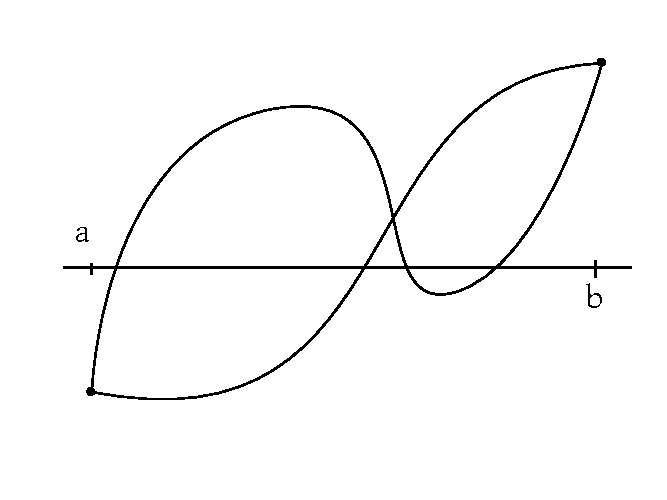
\includegraphics[width=0.5\textwidth]{img/11_ambiguous_solution.pdf}
    \caption{There might be multiple solutions for $f(x) = 0$ for $x \in [a,b]$}
    \label{img:ambsol}
  \end{center}
\end{figure}

$p=1, c < 1$.

Convergence for all $x_0 \in [a,b] \leadsto$ global convergence.
Convergence only for $x_0 \in \mathcal U_\varepsilon(\overline x) \leadsto$ local convergence.

\subsection{Bisection method}

$f(x) = 0, x \in [a,b], f(x) \text{ continuous}, f(a) f(b) < 0$.

Algorithm:
\begin{enumerate}
  \item $a_0 \coloneqq a, b_0 \coloneqq b$
  \item For $k = 0,1,2,\ldots$
  \begin{enumerate}
    \item $x_k = \frac12 (a_k + b_k)$
    \item $f(x_k) = 0 \implies \overline x = x_k$, then terminate
    \item If $f(a_k) f(x_k) < 0$, $a_{k+1} = a_k, b_{k+1} = x_k$ \\ else $a_{k+1} = x_k, b_{k+1} = b_k$
  \end{enumerate}
\end{enumerate}

\[ \card{x_k - \overline x} \leq \frac{b_k - a_k}{2} \implies \card{x_k - \overline x} \leq \frac1{2^{k+1}} \card{b - a} \]
gives global convergence.

\begin{example}
  Let $x \in [1,4]$, $f(x) = x^2 - 4$ and obviously $\overline x = 2$.

  \begin{center}
    \begin{tabular}{ccccc}
      $k$ & $a_k$ & $b_k$ & $x_k$ \\
    \hline
      0 & 1 & 4 & 2.5 & 0.5 \\
      1 & 1 & 2.5 & 1.75 & 0.25 \\
      2 & 1.75 & 2.5 & 2.125 & 0.125 \\
      \vdots
    \end{tabular}
  \end{center}
\end{example}

\begin{example}
  \[ f(x) = \frac x8 (63x^4 - 70x^2 + 15) \]
  Let $[a,b] = [0.8,1], \overline x = \frac1{21} \sqrt{245 + 14\sqrt{70}} \sim 0.906179\ldots$.
  \[ x_0 = 0.9, \card{x_0 - \overline x} \sim 0.006 \]
  \[ x_1 = 0.95, \card{x_1 - \overline x} \sim 0.048\dots \]
  As we can see the error increases. So convergence is not monotone. So, what is our termination criterion?
  The desired convergence property would be:
  \[ \card{x_{k+1} - \overline x} < \card{x_k - \overline x} \]
\end{example}

\subsection{Method of Successive Approximation}

Determination of a root of $f(x) = 0, x \in [a,b]$.
We look for fixed point $x = \varphi(x)$.
Successive approximation takes the approach to define initial value $x_0$
and determines $x_{k+1} \coloneqq \varphi(x_k)$. What about convergence?

\begin{theorem}[Banach fixed point theorem] Let $D$ be a self-mapping:
  \[ D \coloneqq [a,b] \qquad \varphi: [a,b] \to [a,b] \]
  \[ \card{\varphi(x) - \varphi(y)} \leq q \card{x - y} \forall x,y \in [a,b], q < 1 \text{ contraction} \]
  Then the sequence $x_{k+1} = \varphi(x_k)$ of approximate solution for every $x_0 \in [a,b]$ towards a unique
  solution $\overline x = \varphi(\overline x)$.
\end{theorem}
\begin{remark}
  The following error estimates hold:
  \[ \overline x = \varphi(\overline x), x_{k+1} = \varphi(x_k) \]
  \begin{align*}
    \card{x_{k+1} - \overline{x}} &= \card{\varphi(x_k) - \varphi(\overline x)} \leq q \card{x_k - \overline x} \\
      &= q \card{x_k \underbrace{- x_{k+1} + x_{k+1}}_{=0} - \overline x} \\
      &\leq q \card{x_k - x_{k+1}} + q \card{x_{k+1} - \overline x}
  \end{align*}
  \[ \implies \card{x_{k+1} - \overline x} \leq \frac{q}{1 - q} \card{x_{k+1} - x_k} \]
  is an a-posterior error estimate. Alternatively,
  \begin{align*}
    \card{x_{k+1} - \overline x} &\leq q \card{x_k - \overline x} \\
      &\leq q^2 \card{x_{k-1} - \overline x} \\
      &\leq \ldots \\
      &\leq q^{k+1} \card{x_0 - \overline x} \\
      &\leq q^k \underbrace{\card{x^1 - \overline x}}_{\leq \frac{q}{1-q} \card{x_1 - x_0}}
  \end{align*}
  A-priori error estimate:
  \[ \card{x_{k+1} - \overline x} \leq \frac{q^{k+1}}{1 - q} \card{x_1 - x_0} \]
\end{remark}

\begin{example}
  $[a,b] = [1,4], f(x) = x^2 - 4 = 0$.
  \begin{align*}
    x^2 &= 4 \\
    2x^2 &= 4 + x^2 \\
    x &= \frac12 \left(x + \frac4{x^2}\right)
  \end{align*}
  \[ \implies x_{k+1} = \frac12 \left(x_k + \frac{4}{x_k}\right) \qquad x_0 = 4 \]
  $\set{x_{k+1}}$ is monotonically decreasing and bounded by below.
  \[ \varphi(x) = \frac12 \left(x + \frac4x\right) \]
  Contraction?
  \[ \card{\varphi(x) - \varphi(y)} \leq q \card{x - y} \stackrel{x \neq y}{\iff} \frac{\card{\varphi(x) - \varphi(y)}}{\card{x - y}} \leq q \qquad \forall x,y \in [2,4], x \neq y \]
  \[ \max_{\eta \in [2,4]} \card{\varphi'(\eta)} = q \]
  \[ \varphi(x) = \frac12 \left(x + \frac4x\right) \]
  \[ \varphi'(x) = \frac12 \left(1 - \frac4{x^2}\right) \]
  \[ \implies q = \frac38 < 1 \]
  Hence, Banach's Fixed Point Theorem provides linear convergence.
  \[ x_{k+1} = \frac12 \left(x_k + \frac4{x_k} \right) \]
  \[ x_0 = 4 \qquad \card{x_0 - \overline x} = 2 \]
  \[ x_1 = \frac52 = 2.5 \qquad \card{x_1 - \overline x} = 0.5 \]
  \[ x_2 = \frac12 \left(\frac52 + \frac4{\frac52}\right) = \frac{41}{20} = 2.05 \qquad \card{x_2 - \overline x} = 0.05 \]
  \[ x_3 = \frac12 \left(\frac{41}{20} + \frac{4\cdot20}{41}\right) = \frac12 \frac{41^2 + 1600}{820} \qquad \card{x_3 - \overline x} \approx 0.00061 \]
  Is this better than linear convergence?
\end{example}

\begin{proof}[Proof of higher convergence order]
  \begin{align*}
    \card{x_{k+1} - \overline x}
      &= \card{\varphi(x_k) - \varphi(\overline x)} \\
      &= \card{\frac12 \left(x_k + \frac4{x_k}\right) - \frac12 \left(\overline x + \frac4{\overline x}\right)} \\
      &= \frac12 \card{x_k - \overline x + \frac4{x_k} - \frac4{\overline x}} \\
      &= \frac12 \card{x_k - \overline x + 4 \frac{\overline x - x_k}{x_k \overline x}} \\
      &= \frac12 \card{x_k - \overline x} \underbrace{\card{1 - \frac{\overbrace{4}^{=\overline x^2}}{x_k \overline x}}}_{= 1 - \frac{\overline x}{x_k} = \frac1{x_k}\left(x_k - \overline x\right)}
  \end{align*}
  \[ \implies \card{x_{k+1} - \overline x} \leq \frac12 \frac{1}{x_k} \card{x_k - \overline x}^2 \]
  $p=2$ is squared convergence.

  This is the Babylonian method of computing square roots.
\end{proof}

Recursion recurrence $\to$ Taylor

\[ f(x) = f(x_0) + (x - x_0) f'(\eta) \]
\[ x_0 \leadsto x_k \qquad x \leadsto \overline x: f(\overline x) = 0 \]
\[ 0 = f(\overline x) = f(x_k) + (\overline x - x_k) f'(\eta) \]
\[ \overline x = x_k - \frac{f(x_k)}{f'(\eta)}, f'(\eta) \neq 0 \]

Approximation of $f'(\eta) \leadsto$ approximation method

\[ f'(\eta) \sim \frac{f(b) - f(a)}{b - a} \implies x_{k+1} = x_k - \frac{b - a}{f(b) - f(a)} f(x_k) \]
\index{Chord method}
This is the so-called \emph{chord method}.

\begin{figure}[!h]
  \begin{center}
    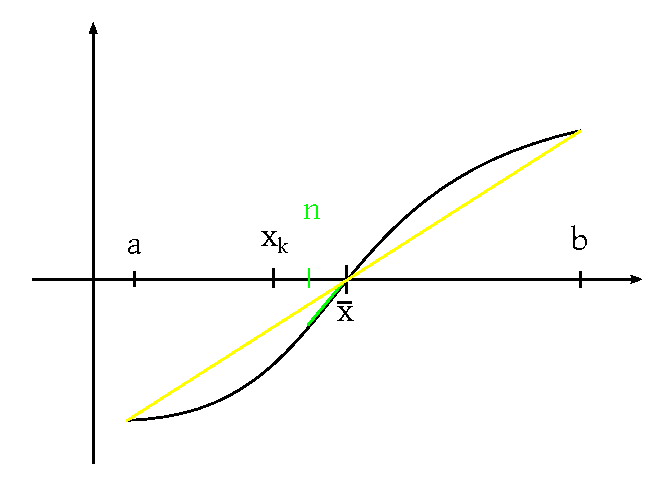
\includegraphics[width=0.5\textwidth]{img/12_approximation.pdf}
    \caption{The green slope is approximated with the yellow slope in the chord method}
    \label{img:approx12}
  \end{center}
\end{figure}

\[ f'(\beta) \sim \frac{f(x_k) - f(x_{k-1})}{x_k - x_{k-1}} \qquad x_{k+1} = x_k - \frac{x_k - x_{k-1}}{f(x_k) - f(x_{k-1})} f(x_k) \]
\index{Secant method}
This is the so-called \emph{secant method}.

\[ f(a) f(b) < 0, f(x_k) f(x_{k-1}) > 0 \implies x_l: f(x_k) f(x_l) < 0 \]
\[ f'(\eta) \approx \frac{f(x_k) - f(x_l)}{x_k - x_l} \qquad l \coloneqq \argmax\set{j: f(x_k) f(x_j) < 0} \]  % TODO: argmax oder maxarg?
\index{Regula Falsi}
This is the so-called \emph{Regula Falsi}

\[ f'(x_k) \neq 0 \implies f'(\eta) \sim f'(x_k) \]
\[ \implies x_{k+1} = x_k - \frac{f(x_k)}{f'(x_k)} \]
\index{Newton method}
This is the so-called \emph{Newton method}.

\begin{theorem}
  Let $f(x)$ be two times differentiable and in the neighborhood of zero value $\overline x$ it holds that
  \[ \frac12 \card{\frac{f''(x)}{f'(\tilde x)}} \leq M. \]
  $x_0, x_1$ satisfy:
  \[ K = \max\set{M \card{x_0 - \overline x}, \sqrt[p]{M \card{x_1 - \overline x}} < 1, p = \frac{1 + \sqrt5}{2} \sim 1.618} \]
  \[ \implies \card{x_{k+1} - \overline x} \leq \frac{1}{M} K^{p^{k+1}} \]
  Secant method.
\end{theorem}

\[ x_{k+1} = \varphi(x_k), \qquad \overline x = \varphi(\overline x) \]
\[ \varphi^{(n)}(\overline x) = 0 \implies \card{x^{k+1} - \overline x} \leq ? \]

\dateref{2018/01/24}

Revision: Non-linear equations:
\[ f(\overline x) = 0 \]
\[ x = \varphi(x) \qquad x_{k+1} = \varphi(x_k) \]

\begin{theorem}
  Let $D = [a,b]$.
  Let $\varphi(x)$ is $p$-times continuously differentiable in $D$. Furthermore we assume
  \[ \varphi'(x) = \varphi''(x) = \ldots = \varphi^{(p-1)}(\overline x) = 0 \text{ in } \overline x = \varphi(\overline x) \]
  and $\varphi^{(p)}(\overline x) \neq 0$.

  Then it holds that
  \[ \abs{x_{k+1} - \overline x} \leq \frac1{p!} \max_{x \in \mathcal U_{\delta}(\overline x)} \card{\varphi^{(p)}(x)} \abs{x_k - \overline x}^p \]
  where $\mathcal U_{\delta}$ defines a neighborhood.
\end{theorem}
\begin{proof}
  \[ x_{k+1} = \varphi(x_k) = \varphi(\overline x) + \sum_{n=1}^{p-1} \frac{1}{n!} (x_k - \overline x)^n \underbrace{\varphi^{(n)}(\overline x)}_{=0} + \frac1{p!} \varphi^{(p)}(\eta)(x_k - \overline x)^p \]
  \[ \implies x_{k+1} - \overline x = \frac1{p!} \varphi^{(p)}(\eta)(x_k - \overline x)^p \]
  $\varphi^{(p)}(\overline x) \neq 0$, $\varphi^{(p)}(x)$ is continuous $\implies \varphi^{(p)}(x) \neq 0$ in $\mathcal U_{\delta}(\overline x)$, hence the assumption follows.
\end{proof}

Application of the Newton method:
\[ x_{k+1} = x_k - \frac{f(x_k)}{f'(x_k)} \eqqcolon \varphi(x_k) \qquad \varphi(x) = x - \frac{f(x)}{f'(x)} \qquad f'(x) \neq 0 \text{ in } \mathcal U_\delta(\overline x) \]
\[ \varphi'(x) = 1 - \frac{f'(x)}{f'(x)} + \frac{f(x) f''(x)}{[f'(x)]^2} = \frac{f(x) f''(x)}{[f'(x)]^2} \]
\[ \varphi'(\overline x) = \frac{f(\overline x) f''(\overline x)}{[f'(\overline x)]^2} = 0 \]
\[ \varphi''(x) = \frac{f''(x) [f'(x)]^2 - 2f(x) [f''(x)]^2 + f(x) f'(x) f^{(3)}(x)}{[f'(x)]^3} \]
\[ \varphi''(\overline x) = \frac{f''(\overline x)}{f'(\overline x)} \neq 0 \text{ in general} \]
$\implies p=2$, hence
\[ \abs{x_{k+1} - \overline x} \leq c \card{x_k - \overline x}^2 \]
Quadratic convergence of the Newton method.

\begin{example}
  \begin{figure}[t]
    \begin{center}
      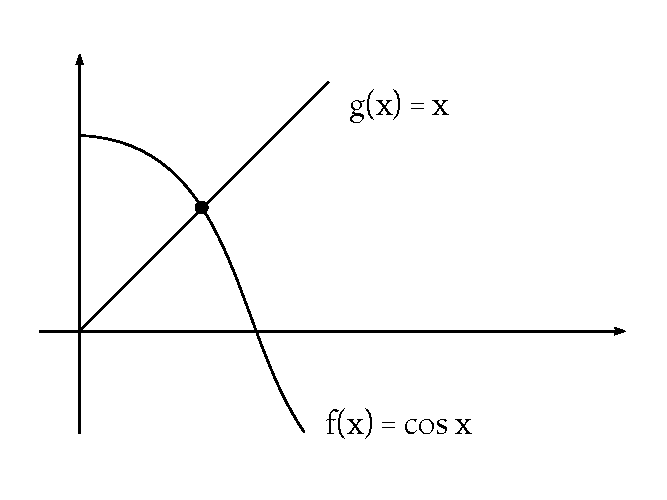
\includegraphics[scale=0.6]{img/13_convergence_example.pdf}
      \caption{Example intersecting $\cos(x)$ and $x$}
      \label{img:intersect}
    \end{center}
  \end{figure}

  \[ x = \cos(x) \]
  \[ x_{k+1} = \cos(x_k) \]
  $\varphi(x) = \cos(x)$;
  contraction for $x \in [0,1]$;
  Banach fixed point theorem: convergence for $x_0 \in [0,1]$;
  Convergence for $x_0 \in \mathbb R$.

  Newton method:
  \[ x_{k+1} = x_k - \frac{f(x_k)}{f'(x_k)} \]
  \[ f(x) = x-cos(x) \]
  \[ f'(x) = 1 + \sin(x) \qquad f'\left(\frac{3\pi}{2}\right) = 0 \]

  This example shows that we only achieve local convergence (even though quadratic convergence by Newton's method is given).
\end{example}

\begin{example}[Babylonian method for computing the square root]
  \begin{align*}
    x_{k+1} &= \frac12 \left(x_k + \frac a{x_k}\right) \\
    \varphi(x) &= \frac12 \left(x + \frac ax\right) \\
    \varphi'(x) &= \frac12 \left(1 - \frac a{x^2}\right) \\
    \overline x &= \sqrt a \\
    \varphi'(\sqrt{\overline{a}}) &= 0 \\
    \varphi''(x) &= \frac a{x^3} \\
    \varphi''(\sqrt a) &= \frac{1}{\sqrt a} \neq 0
  \end{align*}
  $p=2$, quadratic convergence.
\end{example}

\begin{example}
  \[ x^2 = a \qquad f(x) = x^2 - a \qquad f'(x) = 2x \]
  \[ \varphi(x) = x - \frac{f(x)}{f'(x)} = x - \frac{x^2 - a}{2x} = x - \frac12 x + \frac12 \frac{a}{x} = \frac12\left(x + \frac ax\right) \]
  Hence, the Babylonian method of computing square roots corresponds to the Newton method.
\end{example}

Non-linear equation systems:
\[ F(\underline x) = 0 \qquad \underline x \in \mathbb R^n \qquad F(\underline x) = \left(f_i(\underline x)\right)^n_{i=1} \]
\[ f_i(x_1, \ldots, x_n) = 0 \]
\[ 0 = f_i(\overline{\underline{x}}) = \left.f_i(\underline x^k) + \sum_{j=1}^n \left(\overline x_j - x_j^k\right) \frac{\partial}{\partial x_j} f_i(\underline x)\right|_{\underline x = \underline x^k} + \text{ remainder} \]
\[ \iff 0 = f_i(\underline x^k) + \sum_{j=1}^n \left(x_j^{k+1} - x_j^k\right) \underbrace{\left.\frac{\partial}{\partial x_j} f_i(\underline x)\right|_{x = \underline x^k}}_{A_{ij}(\underline x^k)} \]
\[ F(\underline x^k) + A(\underline x^k) \left(\underline x^{k+1} - \underline x^k\right) \stackrel!= \underline 0 \]
\[ \underline x^{k+1} = \underline x^k - \left[A(\underline x^k)\right]^{-1} F(\underline x^k) \]

\dateref{2018/01/29}

Today was the second partial exam of the practicals. No lecture.

\dateref{2018/01/31}

\section{Final conclusions}

\subsection{Approximation of functions}

We considered the problem of approximation of functions.
This problem has local and global solutions. We discussed two methods of interpolation and projections.
Approximation properties in a scale of function spaces (those spaces are called Sobolev-spaces\footnote{We explicitly did not define this space in the lecture.}):
\[ \norm{u - u_h}_{\tau} \leq ch^{s-\tau} \abs{u}_s \qquad 0 \leq \tau \leq s \leq p+1, \tau \leq 1 \]
$\tau$ is bounded by the regularity of the base functions.
Analogue error estimates also hold for $\tau < 0$ in case of projection methods (explicitly \emph{no} interpolation!).
Why is interpolation still popular? Interpolation is local and simple to compute\footnote{if one point changes, only one coefficient needs to be recomputed}, but continuity of the approximating function is required and stability is a big concern.
In contrast, projection is more stable, but global\footnote{if one point changes, an entire linear equation system needs to be resolved}.

Can we combine these approaches? This lead to the development of \emph{Quasi-Interpolation}. You define a parameter:
\[ R_b u(x) = \sum_{k=1}^n F_k(u) e_k(x) \]
This also works for higher dimensions. But the proof techniques become more difficult.
Approximation property is part of computational calculus (dt. \foreignlanguage{ngerman}{numerische Analysis}) of discretization methods for Dgl (?).

\subsection{Numerical integration}

Next, we considered numerical integration.
We discussed Gauss-Legendre in 1D. There are 3 approaches:
\begin{itemize}
  \item Tensor product in $\mathbb R^n$
  \item multidimensional Gauss formula (Radon, 7 points)
  \item singular surface integrals
\end{itemize}

\subsection{Linear Equation Systems}

To solve linear equation systems, we discussed two direct methods: CG method and GMRES. These are just two of many methods, but especially the CG method is very fundamental. In \enquote{Elective Subject} courses, further variants of GMRES are discussed. Then we also discussed preconditioning and its application.

\subsection{Non-linear equation systems}

We discussed the Newton method.

\subsection{Eigenvalues problems}

We did not cover this topic, but will be caught up in \enquote{Elective Subjects}.

Further courses at University of Technology Graz:
\begin{enumerate}
  \item Numerik 1 (Ordinary Differential Equations) [4th semester]
  \item Numerik 2 (Ordinary Differential Equations), Partial Differential Equations [5th semester]
  \item Numerik 3 (Ordinary Differential Equations) [6th semester]
\end{enumerate}

Exams will be held orally and please look up the next exam dates online or request possible exam dates via email.

% TODO \printindex
\end{document}
